%%%%%%%%%%%%%%%%%%%%%%%%%%%%%%%%%%%%%%%%%%%%%%%%%%%%%%%%%%%%%%%%%%%%
% Defesa de Dissertação de Mestrado - PPGC/UFRGS
% Monitoramento de Segurança em Canteiros de Obra
% Inferência Multiestágio em IA na Borda
%%%%%%%%%%%%%%%%%%%%%%%%%%%%%%%%%%%%%%%%%%%%%%%%%%%%%%%%%%%%%%%%%%%%

\documentclass{beamer}

% ============================================================================
% PACOTES
% ============================================================================
\usepackage[T1]{fontenc}
\usepackage[brazil]{babel}
\usepackage[utf8]{inputenc}
\usepackage{graphicx}
\usepackage{amsmath}
\usepackage{amssymb}
\usepackage{tikz}
\usetikzlibrary{
  shapes.geometric,
  arrows.meta,
  positioning,
  fit,
  calc,
  backgrounds,
  decorations.pathreplacing
}
\usepackage{pgfplots}
\pgfplotsset{compat=1.18}
\usepackage{caption}
\usepackage{colortbl}
\usepackage{booktabs}
\usepackage{multirow}
\usepackage{tabularx}
\usepackage{array}
\usepackage{adjustbox}

% ============================================================================
% TEMA
% ============================================================================
\usetheme{Inf}
\graphicspath{{Figures/}}

% ============================================================================
% CORES TikZ (da dissertação)
% ============================================================================
\definecolor{inputcolor}{RGB}{66, 133, 244}
\definecolor{backbonecolor}{RGB}{52, 73, 94}
\definecolor{cspcolor}{RGB}{41, 128, 185}
\definecolor{c3color}{RGB}{26, 82, 118}
\definecolor{neckcolor}{RGB}{142, 68, 173}
\definecolor{panetcolor}{RGB}{155, 89, 182}
\definecolor{headcolor}{RGB}{39, 174, 96}
\definecolor{outputcolor}{RGB}{230, 126, 34}
\definecolor{arrowcolor}{RGB}{127, 140, 141}
\definecolor{skipcolor}{RGB}{192, 57, 43}
\definecolor{labelcolor}{RGB}{44, 62, 80}
\definecolor{bgbox}{RGB}{236, 240, 241}
\definecolor{cpucolor}{RGB}{76, 114, 176}
\definecolor{gpucolor}{RGB}{85, 168, 104}
\definecolor{memcolor}{RGB}{196, 78, 82}
\definecolor{dlacolor}{RGB}{129, 114, 179}
\definecolor{videocolor}{RGB}{204, 153, 0}
\definecolor{iocolor}{RGB}{100, 100, 100}
\definecolor{buscolor}{RGB}{50, 50, 50}
\definecolor{bgblock}{RGB}{245, 245, 250}
\definecolor{rpncolor}{RGB}{155, 89, 182}
\definecolor{roicolor}{RGB}{52, 152, 219}
\definecolor{detectioncolor}{RGB}{22, 160, 133}
\definecolor{gridcolor}{RGB}{241, 196, 15}
\definecolor{stagecolor}{RGB}{52, 73, 94}
\definecolor{charactercolor}{RGB}{127, 140, 141}
\definecolor{sublabelcolor}{RGB}{100, 100, 100}
\definecolor{dividercolor}{RGB}{189, 195, 199}

% ============================================================================
% ESTILOS TikZ (da dissertação)
% ============================================================================
\tikzset{
blocktext/.style={
  align=center,
  font=\small,
  text=labelcolor
},
inputblock/.style={
  draw,
  rounded corners,
  fill=inputcolor!15,
  minimum height=10mm,
  minimum width=22mm,
  blocktext
},
backboneblock/.style={
  draw,
  rounded corners,
  fill=backbonecolor!10,
  minimum height=10mm,
  minimum width=28mm,
  blocktext
},
detectionblock/.style={
  draw,
  rounded corners,
  fill=detectioncolor!12,
  minimum height=10mm,
  minimum width=28mm,
  blocktext
},
outputblock/.style={
  draw,
  rounded corners,
  fill=outputcolor!15,
  minimum height=10mm,
  minimum width=22mm,
  blocktext
},
block/.style={
  draw,
  rounded corners,
  fill=bgblock,
  minimum height=9mm,
  minimum width=22mm,
  blocktext
},
titlelabel/.style={
  font=\bfseries\small,
  text=labelcolor,
  align=center
},
stagelabel/.style={
  font=\bfseries\footnotesize,
  text=stagecolor,
  align=center
},
sublabel/.style={
  font=\footnotesize,
  text=sublabelcolor,
  align=center
},
divider/.style={
  draw=dividercolor,
  line width=0.6pt
},
arrow/.style={
  -{Latex[length=2.0mm,width=1.5mm]},
  line width=0.7pt,
  draw=arrowcolor
},
dashedarrow/.style={
  arrow,
  dashed
}
}

% ============================================================================
% INFORMAÇÕES DO TRABALHO
% ============================================================================
\title[Monitoramento de Segurança com Edge AI]{%
  Monitoramento de Segurança em Canteiros de Obra utilizando
  Inferência Multiestágio em Inteligência Artificial na Borda}

\subtitle{Defesa de Dissertação de Mestrado}

\author[Luiz Guilherme Ito]{%
  Luiz Guilherme Martinho Sampaio Ito\\[4pt]
  {\small Orientador: Prof.~Dr.~José Rodrigo Furlanetto de Azambuja}}

\institute{%
  Instituto de Informática --- UFRGS\\
  Programa de Pós-Graduação em Computação}

\date{Março de 2026}

% ============================================================================
% DOCUMENTO
% ============================================================================
\begin{document}

% ============================================================================
% CAPITULO 1 - INTRODUCAO E MOTIVACAO
% ============================================================================

% --- Slide 1: Titulo ---
{
\setbeamertemplate{footline}{}
\begin{frame}[plain]
  \titlepage
\end{frame}
}

% --- Slide 2: Sumario ---
\begin{frame}{Sum\'{a}rio}
  \tableofcontents
\end{frame}

% ============================================================================
\section{Introdu\c{c}\~{a}o}
% ============================================================================

% --- Slide 3: Contexto ---
\begin{frame}{Contexto}
  \vfill

  \begin{columns}[T]
    \begin{column}{0.55\textwidth}
      {
      \setbeamercolor{block title}{fg=white, bg=inputcolor}
      \setbeamercolor{block body}{bg=inputcolor!8}
      \begin{block}{\centering Constru\c{c}\~{a}o Civil no Mundo}
        \centering\smallskip
        {\color{inputcolor}\fontsize{30}{34}\selectfont\textbf{13\%}}\\[2pt]
        {\small do PIB mundial}\\[6pt]
        {\color{inputcolor}\fontsize{30}{34}\selectfont\textbf{7\%}}\\[2pt]
        {\small da for\c{c}a de trabalho global}\\[2pt]
      \end{block}
      }
    \end{column}
    \begin{column}{0.42\textwidth}
      {
      \setbeamercolor{block title}{fg=white, bg=skipcolor}
      \setbeamercolor{block body}{bg=skipcolor!8}
      \begin{block}{\centering Constru\c{c}\~{a}o Civil no Brasil}
        \centering\smallskip
        {\color{skipcolor}\fontsize{30}{34}\selectfont\textbf{6,2\%}}\\[2pt]
        {\small do PIB nacional}\\[6pt]
        {\color{skipcolor}\fontsize{30}{34}\selectfont\textbf{2,5M}}\\[2pt]
        {\small trabalhadores formais}\\[2pt]
      \end{block}
      }
    \end{column}
  \end{columns}

  \vspace{6mm}

  \begin{center}
    \begin{tikzpicture}
      \node[fill=stagecolor!10, rounded corners=3pt, inner sep=6pt, text width=0.88\textwidth, align=center] {
        {\footnotesize O setor lidera as estat\'{i}sticas de \textbf{acidentes graves e fatais}
        tanto no Brasil quanto mundialmente. Quedas de altura, soterramento,
        choque el\'{e}trico e impacto de objetos s\~{a}o as principais causas.}
      };
    \end{tikzpicture}
  \end{center}
  \vfill
\end{frame}

% --- Slide 4: O Problema ---
\begin{frame}{O Problema}
  \vfill

  % --- Big numbers row ---
  \begin{columns}[c]
    \begin{column}{0.30\textwidth}
      \centering
      \begin{tikzpicture}
        \node[fill=skipcolor!12, rounded corners=4pt, inner sep=8pt, minimum width=32mm] {
          \begin{minipage}{28mm}\centering
            {\color{skipcolor}\fontsize{36}{40}\selectfont\textbf{2,78M}}\\[4pt]
            {\small mortes/ano por\\acidentes de trabalho}\\[2pt]
            {\tiny\color{sublabelcolor} Fonte: OIT, 2024}
          \end{minipage}
        };
      \end{tikzpicture}
    \end{column}

    \begin{column}{0.02\textwidth}
      \centering
      {\color{dividercolor}\rule{0.4pt}{40mm}}
    \end{column}

    \begin{column}{0.30\textwidth}
      \centering
      \begin{tikzpicture}
        \node[fill=inputcolor!10, rounded corners=4pt, inner sep=8pt, minimum width=32mm] {
          \begin{minipage}{28mm}\centering
            {\color{inputcolor}\fontsize{36}{40}\selectfont\textbf{600k}}\\[4pt]
            {\small acidentes registrados\\no Brasil em 2022}\\[2pt]
            {\tiny\color{sublabelcolor} 12\% na constru\c{c}\~{a}o}
          \end{minipage}
        };
      \end{tikzpicture}
    \end{column}

    \begin{column}{0.02\textwidth}
      \centering
      {\color{dividercolor}\rule{0.4pt}{40mm}}
    \end{column}

    \begin{column}{0.30\textwidth}
      \centering
      \begin{tikzpicture}
        \node[fill=outputcolor!12, rounded corners=4pt, inner sep=8pt, minimum width=32mm] {
          \begin{minipage}{28mm}\centering
            {\color{outputcolor}\fontsize{36}{40}\selectfont\textbf{$<$40\%}}\\[4pt]
            {\small taxa de detec\c{c}\~{a}o\\na vigil\^{a}ncia manual}\\[2pt]
            {\tiny\color{sublabelcolor} Teizer, 2015}
          \end{minipage}
        };
      \end{tikzpicture}
    \end{column}
  \end{columns}

  \vspace{6mm}

  % --- Problem statement ---
  \begin{alertblock}{}
    \centering
    \textbf{Inspe\c{c}\~{o}es manuais s\~{a}o intermitentes, reativas e sujeitas a erros humanos.}\\[2pt]
    {\small Como automatizar a vigil\^{a}ncia de seguran\c{c}a em canteiros de obra?}
  \end{alertblock}
  \vfill
\end{frame}

% --- Slide 5: Motivacao ---
\begin{frame}{Motiva\c{c}\~{a}o --- Por que IA na Borda?}
  \vfill

  \begin{center}
    {\small Vis\~{a}o computacional + \textit{deep learning} = vigil\^{a}ncia cont\'{i}nua e autom\'{a}tica.\\[2pt]
    Mas \textbf{onde} processar os dados?}
  \end{center}

  \vspace{4mm}

  \begin{columns}[T]
    \begin{column}{0.46\textwidth}
      {
      \setbeamercolor{block title}{fg=white, bg=skipcolor!85}
      \setbeamercolor{block body}{bg=skipcolor!6}
      \begin{block}{\centering Nuvem}
        \smallskip
        \begin{itemize}
          \item[\color{skipcolor}$\boldsymbol{\times}$] Lat\^{e}ncia: 200--500\,ms
          \item[\color{skipcolor}$\boldsymbol{\times}$] Banda: 3--10\,Mbps/c\^{a}m
          \item[\color{skipcolor}$\boldsymbol{\times}$] Falha se sem internet
          \item[\color{skipcolor}$\boldsymbol{\times}$] Custo recorrente
        \end{itemize}
        \smallskip
      \end{block}
      }
    \end{column}
    \begin{column}{0.46\textwidth}
      {
      \setbeamercolor{block title}{fg=white, bg=headcolor!85}
      \setbeamercolor{block body}{bg=headcolor!6}
      \begin{block}{\centering Borda (Edge AI)}
        \smallskip
        \begin{itemize}
          \item[\color{headcolor}$\boldsymbol{\checkmark}$] Lat\^{e}ncia: $<$100\,ms
          \item[\color{headcolor}$\boldsymbol{\checkmark}$] Sem depend\^{e}ncia de rede
          \item[\color{headcolor}$\boldsymbol{\checkmark}$] Privacidade local
          \item[\color{headcolor}$\boldsymbol{\checkmark}$] Custo fixo (hardware)
        \end{itemize}
        \smallskip
      \end{block}
      }
    \end{column}
  \end{columns}

  \vspace{5mm}

  \begin{center}
    \begin{tikzpicture}
      \node[fill=headcolor!12, rounded corners=3pt, inner sep=6pt, text width=0.82\textwidth, align=center] {
        {\small\textbf{Canteiros de obra} t\^{e}m conectividade inst\'{a}vel e exigem resposta imediata.\\
        A \textbf{computa\c{c}\~{a}o de borda} \'{e} a escolha natural.}
      };
    \end{tikzpicture}
  \end{center}
  \vfill
\end{frame}

% --- Slide 6: Hipotese ---
\begin{frame}{Hip\'{o}tese}
  \vfill

  \begin{center}
    \begin{tikzpicture}
      \node[fill=stagecolor!8, rounded corners=4pt, inner sep=8pt, text width=0.9\textwidth, align=center] {
        {\small Uma arquitetura de \textbf{infer\^{e}ncia em cascata} na borda,\\[2pt]
        com modelo prim\'{a}rio generalista + modelos secund\'{a}rios especializados,\\[2pt]
        pode monitorar seguran\c{c}a em \textbf{tempo real} com m\'{u}ltiplas categorias.}
      };
    \end{tikzpicture}
  \end{center}

  \vspace{3mm}

  % --- Cascade Diagram - Vertical flow ---
  \begin{center}
    \resizebox{0.92\textwidth}{!}{%
    \begin{tikzpicture}[
      node distance=6mm and 12mm,
      every node/.style={font=\small, align=center},
      sgienode/.style={draw, rounded corners=3pt, minimum height=13mm, minimum width=30mm, font=\small, align=center},
    ]
      % Camera
      \node[inputblock, minimum width=26mm, minimum height=14mm] (cam) {
        \textbf{C\^{a}mera}\\{\scriptsize RTSP Stream}
      };

      % PGIE
      \node[backboneblock, right=14mm of cam, minimum width=32mm, minimum height=14mm] (pgie) {
        \textbf{PGIE}\\{\scriptsize 5 classes gerais}
      };

      % SGIEs - spread vertically
      \node[sgienode, fill=roicolor!15, right=16mm of pgie, yshift=18mm] (sgie1) {
        \textbf{SGIE-EPI}\\{\scriptsize 14 classes}
      };
      \node[sgienode, fill=neckcolor!12, right=16mm of pgie] (sgie2) {
        \textbf{SGIE-Maq}\\{\scriptsize 9 classes}
      };
      \node[sgienode, fill=gridcolor!15, right=16mm of pgie, yshift=-18mm] (sgie3) {
        \textbf{SGIE-Fer}\\{\scriptsize 23 classes}
      };

      % Output
      \node[outputblock, right=16mm of sgie2, minimum width=26mm, minimum height=14mm] (alerta) {
        \textbf{Alerta}\\{\scriptsize Tempo Real}
      };

      % Arrows
      \draw[arrow, line width=1pt] (cam) -- (pgie);

      % PGIE to SGIEs with ROI labels
      \draw[arrow, line width=1pt] (pgie.east) -- (sgie1.west)
        node[midway, above, font=\tiny\itshape, text=sublabelcolor] {ROI: pessoa};
      \draw[arrow, line width=1pt] (pgie.east) -- (sgie2.west)
        node[midway, above, font=\tiny\itshape, text=sublabelcolor] {ROI: ve\'{i}culo};
      \draw[arrow, line width=1pt] (pgie.east) -- (sgie3.west)
        node[midway, below, font=\tiny\itshape, text=sublabelcolor] {ROI: ferramenta};

      % SGIEs to Alert
      \draw[arrow, line width=1pt] (sgie1.east) -- (alerta.west |- sgie1.east);
      \draw[arrow, line width=1pt] (sgie2.east) -- (alerta.west);
      \draw[arrow, line width=1pt] (sgie3.east) -- (alerta.west |- sgie3.east);

      % Annotations below
      \node[below=3mm of cam, font=\tiny, text=sublabelcolor] {Entrada};
      \node[below=3mm of pgie, font=\tiny, text=sublabelcolor] {Detector Prim\'{a}rio};
      \node[below=3mm of sgie3, font=\tiny, text=sublabelcolor] {Detectores Secund\'{a}rios};
      \node[below=3mm of alerta, font=\tiny, text=sublabelcolor] {Sa\'{i}da};

      % Total classes annotation
      \node[below=22mm of sgie2, font=\scriptsize\bfseries, text=stagecolor] {
        46 categorias \'{u}nicas --- 4 modelos YOLOv8
      };
    \end{tikzpicture}
    }
  \end{center}

  \vspace{1mm}
  \centering
  {\footnotesize\color{stagecolor}\textbf{Infer\^{e}ncia em cascata na borda} --- NVIDIA Jetson AGX Xavier | DeepStream SDK}
  \vfill
\end{frame}

% ============================================================================
% CAPITULO 2 - OBJETIVOS E CONTRIBUICOES
% ============================================================================

\section{Objetivos}

% --- Slide 7: Objetivo Geral ---
\begin{frame}{Objetivo Geral}
  \vfill

  \begin{center}
    \begin{tikzpicture}
      \node[fill=stagecolor!8, rounded corners=4pt, inner sep=8pt, text width=0.88\textwidth, align=center] {
        {\small Projetar, implementar e validar um sistema de \textbf{an\'{a}lise de v\'{i}deo inteligente}\\[2pt]
        baseado em \textbf{computa\c{c}\~{a}o de borda} com infer\^{e}ncia em cascata para\\[2pt]
        monitoramento de seguran\c{c}a em tempo real em canteiros de obras.}
      };
    \end{tikzpicture}
  \end{center}

  \vspace{6mm}

  \begin{columns}[c]
    \begin{column}{0.30\textwidth}
      {
      \setbeamercolor{block title}{fg=white, bg=inputcolor}
      \setbeamercolor{block body}{bg=inputcolor!8}
      \begin{block}{\centering Onde}
        \centering\medskip
        {\color{inputcolor}\fontsize{22}{26}\selectfont\textbf{Edge}}\\[4pt]
        {\small Computa\c{c}\~{a}o na borda\\Jetson AGX Xavier}\\[2pt]
        {\tiny\color{sublabelcolor} 30W | 512-core GPU}
        \medskip
      \end{block}
      }
    \end{column}
    \begin{column}{0.30\textwidth}
      {
      \setbeamercolor{block title}{fg=white, bg=headcolor}
      \setbeamercolor{block body}{bg=headcolor!8}
      \begin{block}{\centering O qu\^{e}}
        \centering\medskip
        {\color{headcolor}\fontsize{22}{26}\selectfont\textbf{20+ FPS}}\\[4pt]
        {\small Detec\c{c}\~{a}o em\\tempo real}\\[2pt]
        {\tiny\color{sublabelcolor} 4 modelos simult\^{a}neos}
        \medskip
      \end{block}
      }
    \end{column}
    \begin{column}{0.30\textwidth}
      {
      \setbeamercolor{block title}{fg=white, bg=outputcolor}
      \setbeamercolor{block body}{bg=outputcolor!8}
      \begin{block}{\centering Para qu\^{e}}
        \centering\medskip
        {\color{outputcolor}\fontsize{22}{26}\selectfont\textbf{46}}\\[4pt]
        {\small Categorias de\\seguran\c{c}a monitoradas}\\[2pt]
        {\tiny\color{sublabelcolor} EPIs, m\'{a}quinas, ferramentas}
        \medskip
      \end{block}
      }
    \end{column}
  \end{columns}
  \vfill
\end{frame}

% --- Slide 8: Objetivos Especificos (1/2) ---
\begin{frame}{Objetivos Espec\'{i}ficos \hfill {\normalsize\color{sublabelcolor} 1/2}}
  \vfill

  % --- OE1: Modelos ---
  {
  \setbeamercolor{block title}{fg=white, bg=backbonecolor}
  \setbeamercolor{block body}{bg=backbonecolor!6}
  \begin{block}{{\small\textbf{OE1}} --- Treinamento dos Modelos de Detec\c{c}\~{a}o}
    \smallskip
    \begin{columns}[c]
      \begin{column}{0.48\textwidth}
        \begin{itemize}
          \item[\color{backbonecolor}$\blacktriangleright$] Treinar o \textbf{PGIE} para 5 classes gerais\\
            {\tiny pessoa, ve\'{i}culo, capacete, colete, ferramenta}
        \end{itemize}
      \end{column}
      \begin{column}{0.48\textwidth}
        \begin{itemize}
          \item[\color{backbonecolor}$\blacktriangleright$] Treinar 3 \textbf{SGIEs} especializados:\\
            {\tiny EPI (14 cls) | Maquin\'{a}rio (9 cls) | Ferramentas (23 cls)}
        \end{itemize}
      \end{column}
    \end{columns}
    \smallskip
  \end{block}
  }

  \vspace{3mm}

  % --- OE2: Pipeline ---
  {
  \setbeamercolor{block title}{fg=white, bg=neckcolor}
  \setbeamercolor{block body}{bg=neckcolor!6}
  \begin{block}{{\small\textbf{OE2}} --- Pipeline de Infer\^{e}ncia em Cascata}
    \smallskip
    \begin{itemize}
      \item[\color{neckcolor}$\blacktriangleright$] Implementar pipeline \textbf{DeepStream SDK} com infer\^{e}ncia multiest\'{a}gio
      \item[\color{neckcolor}$\blacktriangleright$] Orquestra\c{c}\~{a}o: decodifica\c{c}\~{a}o $\to$ infer\^{e}ncia prim\'{a}ria $\to$ infer\^{e}ncia secund\'{a}ria $\to$ visualiza\c{c}\~{a}o
    \end{itemize}
    \smallskip
  \end{block}
  }

  \vspace{3mm}

  % --- OE3: Parser ---
  {
  \setbeamercolor{block title}{fg=white, bg=detectioncolor}
  \setbeamercolor{block body}{bg=detectioncolor!6}
  \begin{block}{{\small\textbf{OE3}} --- Integra\c{c}\~{a}o YOLO--DeepStream}
    \smallskip
    \begin{itemize}
      \item[\color{detectioncolor}$\blacktriangleright$] Desenvolver fun\c{c}\~{o}es de \textit{parsing} customizadas em \textbf{C++} para modelos YOLOv8
      \item[\color{detectioncolor}$\blacktriangleright$] Roteamento autom\'{a}tico PGIE $\to$ SGIEs baseado na classe detectada
    \end{itemize}
    \smallskip
  \end{block}
  }

  \vfill
\end{frame}

% --- Slide 9: Objetivos Especificos (2/2) ---
\begin{frame}{Objetivos Espec\'{i}ficos \hfill {\normalsize\color{sublabelcolor} 2/2}}
  \vfill

  % --- OE4: Avaliacao ---
  {
  \setbeamercolor{block title}{fg=white, bg=outputcolor}
  \setbeamercolor{block body}{bg=outputcolor!6}
  \begin{block}{{\small\textbf{OE4}} --- Avalia\c{c}\~{a}o de Desempenho}
    \smallskip
    \begin{itemize}
      \item[\color{outputcolor}$\blacktriangleright$] Medir \textbf{acur\'{a}cia} (mAP) de cada modelo individualmente
      \item[\color{outputcolor}$\blacktriangleright$] Medir \textbf{velocidade} (FPS) e lat\^{e}ncia do pipeline completo
      \item[\color{outputcolor}$\blacktriangleright$] Avaliar uso de recursos: GPU, mem\'{o}ria, consumo energ\'{e}tico
    \end{itemize}
    \smallskip
  \end{block}
  }

  \vspace{5mm}

  % --- Summary visual ---
  \begin{center}
    \resizebox{0.85\textwidth}{!}{%
    \begin{tikzpicture}[node distance=8mm]
      \node[fill=backbonecolor!15, rounded corners=3pt, minimum height=11mm, minimum width=28mm, align=center, font=\small] (oe1) {\textbf{OE1}\\{\scriptsize 4 modelos}};
      \node[fill=neckcolor!12, rounded corners=3pt, minimum height=11mm, minimum width=28mm, align=center, font=\small, right=10mm of oe1] (oe2) {\textbf{OE2}\\{\scriptsize Pipeline}};
      \node[fill=detectioncolor!12, rounded corners=3pt, minimum height=11mm, minimum width=28mm, align=center, font=\small, right=10mm of oe2] (oe3) {\textbf{OE3}\\{\scriptsize Parser C++}};
      \node[fill=outputcolor!15, rounded corners=3pt, minimum height=11mm, minimum width=28mm, align=center, font=\small, right=10mm of oe3] (oe4) {\textbf{OE4}\\{\scriptsize Valida\c{c}\~{a}o}};

      \draw[arrow, line width=1pt] (oe1) -- (oe2);
      \draw[arrow, line width=1pt] (oe2) -- (oe3);
      \draw[arrow, line width=1pt] (oe3) -- (oe4);
    \end{tikzpicture}
    }
  \end{center}

  \vspace{2mm}

  \begin{center}
    {\footnotesize\color{stagecolor} Cada objetivo espec\'{i}fico alimenta o seguinte --- fluxo sequencial de desenvolvimento.}
  \end{center}
  \vfill
\end{frame}

% --- Slide 10: Contribuicoes ---
\begin{frame}{Contribui\c{c}\~{o}es}
  \vfill

  \begin{columns}[T]
    \begin{column}{0.48\textwidth}
      % --- C1 ---
      \begin{tikzpicture}
        \fill[inputcolor] (0,0) rectangle (0.12,3.0);
        \node[right, text width=42mm, align=left, font=\small] at (0.25,1.5) {
          \textbf{Arquitetura em Cascata}\\[3pt]
          {\footnotesize PGIE + 3 SGIEs especializados\\operando em ROIs recortadas}\\[5pt]
          {\color{inputcolor}\fontsize{20}{24}\selectfont\textbf{4}} {\small modelos}\\
          {\color{inputcolor}\fontsize{20}{24}\selectfont\textbf{46}} {\small categorias}
        };
      \end{tikzpicture}

      \vspace{4mm}

      % --- C3 ---
      \begin{tikzpicture}
        \fill[neckcolor] (0,0) rectangle (0.12,2.6);
        \node[right, text width=42mm, align=left, font=\small] at (0.25,1.3) {
          \textbf{Pipeline DeepStream}\\[3pt]
          {\footnotesize Processamento acelerado por\\hardware com TensorRT FP16}\\[5pt]
          {\color{neckcolor}\fontsize{20}{24}\selectfont\textbf{58}} {\small ms lat\^{e}ncia}
        };
      \end{tikzpicture}
    \end{column}

    \begin{column}{0.48\textwidth}
      % --- C2 ---
      \begin{tikzpicture}
        \fill[headcolor] (0,0) rectangle (0.12,3.0);
        \node[right, text width=42mm, align=left, font=\small] at (0.25,1.5) {
          \textbf{Modelos Treinados}\\[3pt]
          {\footnotesize YOLOv8 com \textit{transfer learning}\\e otimiza\c{c}\~{a}o TensorRT}\\[5pt]
          {\color{headcolor}\fontsize{20}{24}\selectfont\textbf{FP16}} {\small precis\~{a}o}\\
          {\color{headcolor}\fontsize{20}{24}\selectfont\textbf{mAP}} {\small validado}
        };
      \end{tikzpicture}

      \vspace{4mm}

      % --- C4 ---
      \begin{tikzpicture}
        \fill[outputcolor] (0,0) rectangle (0.12,2.6);
        \node[right, text width=42mm, align=left, font=\small] at (0.25,1.3) {
          \textbf{Valida\c{c}\~{a}o em Borda}\\[3pt]
          {\footnotesize M\'{e}tricas reais no\\Jetson AGX Xavier}\\[5pt]
          {\color{outputcolor}\fontsize{20}{24}\selectfont\textbf{20}} {\small FPS} \quad
          {\color{outputcolor}\fontsize{20}{24}\selectfont\textbf{24}} {\small W}
        };
      \end{tikzpicture}
    \end{column}
  \end{columns}
  \vfill
\end{frame}

% --- Slide 11: Escopo ---
\begin{frame}{Escopo do Trabalho}
  \vfill

  \begin{columns}[T]
    \begin{column}{0.46\textwidth}
      {
      \setbeamercolor{block title}{fg=white, bg=headcolor}
      \setbeamercolor{block body}{bg=headcolor!6}
      \begin{block}{\centering Dentro do Escopo}
        \medskip
        \begin{itemize}
          \item[\color{headcolor}$\boldsymbol{\checkmark}$] Detec\c{c}\~{a}o de EPIs\\
            {\tiny capacete, colete, luvas, botas, \'{o}culos\ldots}
          \item[\color{headcolor}$\boldsymbol{\checkmark}$] Detec\c{c}\~{a}o de maquin\'{a}rio\\
            {\tiny escavadeiras, caminh\~{o}es, guindastes\ldots}
          \item[\color{headcolor}$\boldsymbol{\checkmark}$] Detec\c{c}\~{a}o de ferramentas\\
            {\tiny furadeiras, serras, escadas\ldots}
          \item[\color{headcolor}$\boldsymbol{\checkmark}$] Infer\^{e}ncia em tempo real
          \item[\color{headcolor}$\boldsymbol{\checkmark}$] Execu\c{c}\~{a}o em dispositivo de borda
          \item[\color{headcolor}$\boldsymbol{\checkmark}$] An\'{a}lise de desempenho
        \end{itemize}
        \medskip
      \end{block}
      }
    \end{column}
    \begin{column}{0.46\textwidth}
      {
      \setbeamercolor{block title}{fg=white, bg=skipcolor!80}
      \setbeamercolor{block body}{bg=skipcolor!6}
      \begin{block}{\centering Fora do Escopo}
        \medskip
        \begin{itemize}
          \item[\color{skipcolor}$\boldsymbol{\times}$] Reconhecimento de a\c{c}\~{o}es\\
            {\tiny posturas perigosas, quedas}
          \item[\color{skipcolor}$\boldsymbol{\times}$] Rastreamento de\\identidade (Re-ID)
          \item[\color{skipcolor}$\boldsymbol{\times}$] Integra\c{c}\~{a}o com sistemas\\de gest\~{a}o (ERP/BIM)
          \item[\color{skipcolor}$\boldsymbol{\times}$] Deploy multi-c\^{a}mera\\em larga escala
          \item[\color{skipcolor}$\boldsymbol{\times}$] Treinamento \textit{online}\\(atualiza\c{c}\~{a}o cont\'{i}nua)
          \item[\color{skipcolor}$\boldsymbol{\times}$] Interface para usu\'{a}rio final
        \end{itemize}
        \medskip
      \end{block}
      }
    \end{column}
  \end{columns}
  \vfill
\end{frame}

% ============================================================================
% CAPÍTULO 3 - FUNDAMENTAÇÃO TEÓRICA
% ============================================================================

\section{Fundamentação Teórica}

% --- Slide: Detectores de Objetos ---
\begin{frame}{Detectores de Objetos}
  \vspace{-2mm}
  {\small\color{sublabelcolor}%
    Evolução dos detectores: \textbf{Two-stage} (alta precisão) vs \textbf{Single-stage} (baixa latência)}

  \vfill
  \begin{center}
    \resizebox{!}{0.65\textheight}{% ============================================================================
% Diagrama Comparativo: Detectores de Dois Estágios vs Um Estágio
% Para uso em dissertação de mestrado - PPGC/UFRGS
% Uso: % ============================================================================
% Diagrama Comparativo: Detectores de Dois Estágios vs Um Estágio
% Para uso em dissertação de mestrado - PPGC/UFRGS
% Uso: \input{figuras/diagrama_detectores.tex}
% ============================================================================

\begin{tikzpicture}[
    node distance=0.6cm and 0.8cm,
    scale=0.85, transform shape,
    % Estilos dos blocos
    block/.style={
        rectangle,
        rounded corners=3pt,
        minimum width=2.6cm,
        minimum height=0.7cm,
        text centered,
        font=\small\sffamily,
        text=white,
        draw=none,
    },
    inputblock/.style={block, fill=inputcolor, minimum height=0.9cm},
    backboneblock/.style={block, fill=backbonecolor},
    rpnblock/.style={block, fill=rpncolor},
    roiblock/.style={block, fill=roicolor},
    headblock/.style={block, fill=headcolor},
    outputblock/.style={block, fill=outputcolor, minimum height=0.8cm},
    detectionblock/.style={block, fill=detectioncolor},
    gridblock/.style={block, fill=gridcolor},
    % Estilos das setas
    arrow/.style={-{Stealth[length=2mm, width=1.5mm]}, thick, arrowcolor},
    dashedarrow/.style={-{Stealth[length=2mm, width=1.5mm]}, thick, arrowcolor, dashed},
    % Estilos das labels
    titlelabel/.style={font=\normalsize\sffamily\bfseries, text=labelcolor},
    stagelabel/.style={font=\tiny\sffamily\bfseries, text=white, fill=stagecolor, rounded corners=2pt, inner sep=3pt},
    sublabel/.style={font=\tiny\sffamily, text=sublabelcolor},
    divider/.style={thick, dashed, dividercolor},
]

% ============================================================================
% TÍTULO
% ============================================================================
\node[titlelabel] at (0, 0.3) {Comparação de Arquiteturas de Detectores};

% ============================================================================
% DOIS ESTÁGIOS (Faster R-CNN)
% ============================================================================
\begin{scope}[shift={(-4, 0)}]
    \node[titlelabel] at (0, -0.5) {Dois Estágios};
    \node[sublabel] at (0, -0.9) {(Faster R-CNN)};

    \node[stagelabel] at (-1.8, -1.6) {Estágio 1};
    \node[inputblock] (input2) at (0, -1.6) {Imagem};
    \node[backboneblock] (bb2) at (0, -2.7) {Backbone};
    \node[rpnblock] (rpn) at (0, -3.8) {RPN};
    \node[sublabel, below=0.02cm of rpn] {Propostas de regiões};

    \node[stagelabel] at (-1.8, -4.9) {Estágio 2};
    \node[roiblock] (roi) at (0, -5.0) {ROI Pooling};
    \node[headblock] (head2) at (0, -6.1) {Classificação};
    \node[outputblock] (out2) at (0, -7.2) {Detecções};

    \draw[arrow] (input2) -- (bb2);
    \draw[arrow] (bb2) -- (rpn);
    \draw[arrow] (rpn) -- (roi);
    \draw[arrow] (roi) -- (head2);
    \draw[arrow] (head2) -- (out2);
    \draw[dashedarrow] (bb2.east) -- ++(0.5,0) |- (roi.east);

    \node[sublabel] at (0, -8.0) {Alta precisão | Maior latência};
\end{scope}

% ============================================================================
% LINHA DIVISÓRIA
% ============================================================================
\draw[divider] (0, -0.3) -- (0, -8.2);

% ============================================================================
% UM ESTÁGIO (YOLO)
% ============================================================================
\begin{scope}[shift={(4, 0)}]
    \node[titlelabel] at (0, -0.5) {Um Estágio};
    \node[sublabel] at (0, -0.9) {(YOLO, SSD)};

    \node[stagelabel] at (1.8, -1.6) {Único};
    \node[inputblock] (input1) at (0, -1.6) {Imagem};
    \node[backboneblock] (bb1) at (0, -2.7) {Backbone};
    \node[detectionblock] (det) at (0, -3.8) {Detecção Direta};
    \node[sublabel, below=0.02cm of det] {Predição em grid};
    \node[gridblock] (grid) at (0, -5.0) {Grid $S \times S$};
    \node[outputblock] (out1) at (0, -6.1) {Boxes + Classes};

    \draw[arrow] (input1) -- (bb1);
    \draw[arrow] (bb1) -- (det);
    \draw[arrow] (det) -- (grid);
    \draw[arrow] (grid) -- (out1);
    \draw[dashedarrow] (bb1.west) -- ++(-0.5,0) |- (det.west);
    \node[sublabel, rotate=90] at (-1.0, -3.2) {Multi-escala};

    \node[sublabel] at (0, -6.9) {Baixa latência | Eficiente};
\end{scope}

\end{tikzpicture}

% ============================================================================

\begin{tikzpicture}[
    node distance=0.6cm and 0.8cm,
    scale=0.85, transform shape,
    % Estilos dos blocos
    block/.style={
        rectangle,
        rounded corners=3pt,
        minimum width=2.6cm,
        minimum height=0.7cm,
        text centered,
        font=\small\sffamily,
        text=white,
        draw=none,
    },
    inputblock/.style={block, fill=inputcolor, minimum height=0.9cm},
    backboneblock/.style={block, fill=backbonecolor},
    rpnblock/.style={block, fill=rpncolor},
    roiblock/.style={block, fill=roicolor},
    headblock/.style={block, fill=headcolor},
    outputblock/.style={block, fill=outputcolor, minimum height=0.8cm},
    detectionblock/.style={block, fill=detectioncolor},
    gridblock/.style={block, fill=gridcolor},
    % Estilos das setas
    arrow/.style={-{Stealth[length=2mm, width=1.5mm]}, thick, arrowcolor},
    dashedarrow/.style={-{Stealth[length=2mm, width=1.5mm]}, thick, arrowcolor, dashed},
    % Estilos das labels
    titlelabel/.style={font=\normalsize\sffamily\bfseries, text=labelcolor},
    stagelabel/.style={font=\tiny\sffamily\bfseries, text=white, fill=stagecolor, rounded corners=2pt, inner sep=3pt},
    sublabel/.style={font=\tiny\sffamily, text=sublabelcolor},
    divider/.style={thick, dashed, dividercolor},
]

% ============================================================================
% TÍTULO
% ============================================================================
\node[titlelabel] at (0, 0.3) {Comparação de Arquiteturas de Detectores};

% ============================================================================
% DOIS ESTÁGIOS (Faster R-CNN)
% ============================================================================
\begin{scope}[shift={(-4, 0)}]
    \node[titlelabel] at (0, -0.5) {Dois Estágios};
    \node[sublabel] at (0, -0.9) {(Faster R-CNN)};

    \node[stagelabel] at (-1.8, -1.6) {Estágio 1};
    \node[inputblock] (input2) at (0, -1.6) {Imagem};
    \node[backboneblock] (bb2) at (0, -2.7) {Backbone};
    \node[rpnblock] (rpn) at (0, -3.8) {RPN};
    \node[sublabel, below=0.02cm of rpn] {Propostas de regiões};

    \node[stagelabel] at (-1.8, -4.9) {Estágio 2};
    \node[roiblock] (roi) at (0, -5.0) {ROI Pooling};
    \node[headblock] (head2) at (0, -6.1) {Classificação};
    \node[outputblock] (out2) at (0, -7.2) {Detecções};

    \draw[arrow] (input2) -- (bb2);
    \draw[arrow] (bb2) -- (rpn);
    \draw[arrow] (rpn) -- (roi);
    \draw[arrow] (roi) -- (head2);
    \draw[arrow] (head2) -- (out2);
    \draw[dashedarrow] (bb2.east) -- ++(0.5,0) |- (roi.east);

    \node[sublabel] at (0, -8.0) {Alta precisão | Maior latência};
\end{scope}

% ============================================================================
% LINHA DIVISÓRIA
% ============================================================================
\draw[divider] (0, -0.3) -- (0, -8.2);

% ============================================================================
% UM ESTÁGIO (YOLO)
% ============================================================================
\begin{scope}[shift={(4, 0)}]
    \node[titlelabel] at (0, -0.5) {Um Estágio};
    \node[sublabel] at (0, -0.9) {(YOLO, SSD)};

    \node[stagelabel] at (1.8, -1.6) {Único};
    \node[inputblock] (input1) at (0, -1.6) {Imagem};
    \node[backboneblock] (bb1) at (0, -2.7) {Backbone};
    \node[detectionblock] (det) at (0, -3.8) {Detecção Direta};
    \node[sublabel, below=0.02cm of det] {Predição em grid};
    \node[gridblock] (grid) at (0, -5.0) {Grid $S \times S$};
    \node[outputblock] (out1) at (0, -6.1) {Boxes + Classes};

    \draw[arrow] (input1) -- (bb1);
    \draw[arrow] (bb1) -- (det);
    \draw[arrow] (det) -- (grid);
    \draw[arrow] (grid) -- (out1);
    \draw[dashedarrow] (bb1.west) -- ++(-0.5,0) |- (det.west);
    \node[sublabel, rotate=90] at (-1.0, -3.2) {Multi-escala};

    \node[sublabel] at (0, -6.9) {Baixa latência | Eficiente};
\end{scope}

\end{tikzpicture}
}
  \end{center}
  \vfill

  \begin{beamercolorbox}[wd=\textwidth, rounded=true, shadow=false]{block body}
    \centering
    {\footnotesize\color{stagecolor}%
      \textbf{YOLO} escolhido: melhor \textit{trade-off} velocidade/acurácia para inferência em tempo real na borda}
  \end{beamercolorbox}
\end{frame}

% --- Slide: Arquitetura YOLOv8 ---
\begin{frame}{Arquitetura YOLOv8}
  \vspace{-2mm}
  {\small\color{sublabelcolor}%
    Três componentes: \textbf{Backbone} (extração) + \textbf{Neck} (fusão multi-escala) + \textbf{Decoupled Head} (detecção)}

  \vfill
  \begin{center}
    \resizebox{0.92\textwidth}{!}{% ============================================================================
% Diagrama da Arquitetura YOLOv8s (Simplificado)
% Para uso em dissertação de mestrado - PPGC/UFRGS
% Uso: % ============================================================================
% Diagrama da Arquitetura YOLOv8s (Simplificado)
% Para uso em dissertação de mestrado - PPGC/UFRGS
% Uso: \input{figuras/diagrama_yolov8.tex}
% ============================================================================

\begin{tikzpicture}[
    node distance=0.5cm and 0.6cm,
    scale=0.9, transform shape,
    % Estilos dos blocos
    block/.style={
        rectangle,
        rounded corners=3pt,
        minimum width=1.6cm,
        minimum height=0.6cm,
        align=center,
        font=\small\sffamily,
        text=white,
        draw=none,
    },
    inputblock/.style={block, fill=inputcolor, minimum width=1.8cm, minimum height=0.8cm},
    cbsblock/.style={block, fill=backbonecolor, minimum width=1.2cm},
    c2fblock/.style={block, fill=c3color, minimum width=1.4cm},
    sppfblock/.style={block, fill=backbonecolor!80!black, minimum width=1.4cm},
    neckblock/.style={block, fill=neckcolor, minimum width=1.4cm},
    headblock/.style={block, fill=headcolor, minimum width=1.8cm, minimum height=0.7cm},
    outputblock/.style={block, fill=outputcolor, minimum width=2.2cm, minimum height=0.8cm},
    % Estilos das setas
    arrow/.style={-{Stealth[length=1.8mm, width=1.2mm]}, thick, arrowcolor},
    skiparrow/.style={-{Stealth[length=1.8mm, width=1.2mm]}, thick, skipcolor},
    % Estilos das labels
    sectionlabel/.style={font=\small\sffamily\bfseries, text=labelcolor},
    sizelabel/.style={font=\scriptsize\sffamily, text=sublabelcolor},
]

% ============================================================================
% ENTRADA
% ============================================================================
\node[inputblock] (input) {Imagem\\640$\times$640};
\node[sectionlabel, above=0.3cm of input] {Entrada};

% ============================================================================
% BACKBONE
% ============================================================================
\node[cbsblock, right=0.8cm of input] (cbs1) {CBS};
\node[c2fblock, right=0.4cm of cbs1] (c2f1) {C2f};
\node[sizelabel, below=0.02cm of c2f1] {\tiny P3};

\node[cbsblock, right=0.4cm of c2f1] (cbs2) {CBS};
\node[c2fblock, right=0.4cm of cbs2] (c2f2) {C2f};
\node[sizelabel, below=0.02cm of c2f2] {\tiny P4};

\node[cbsblock, right=0.4cm of c2f2] (cbs3) {CBS};
\node[c2fblock, right=0.4cm of cbs3] (c2f3) {C2f};
\node[sppfblock, right=0.4cm of c2f3] (sppf) {SPPF};
\node[sizelabel, below=0.02cm of sppf] {\tiny P5};

% Backbone label
\node[sectionlabel] at ($(cbs2)!0.5!(c2f3) + (0, 0.8)$) {Backbone (CSPDarknet)};

% ============================================================================
% NECK (FPN + PANet)
% ============================================================================
\node[neckblock, below=1.0cm of c2f2] (neck1) {FPN};
\node[neckblock, right=0.6cm of neck1] (neck2) {PANet};
\node[sectionlabel] at ($(neck1)!0.5!(neck2) + (0, 0.7)$) {Neck};

% ============================================================================
% HEAD
% ============================================================================
\node[headblock, below=1.0cm of neck1] (head1) {Head\\80$\times$80};
\node[headblock, right=0.5cm of head1] (head2) {Head\\40$\times$40};
\node[headblock, right=0.5cm of head2] (head3) {Head\\20$\times$20};
\node[sectionlabel] at ($(head2) + (0, 0.7)$) {Decoupled Head};

\node[sizelabel, below=0.1cm of head1] {Pequenos};
\node[sizelabel, below=0.1cm of head2] {Médios};
\node[sizelabel, below=0.1cm of head3] {Grandes};

% ============================================================================
% SAÍDA
% ============================================================================
\node[outputblock, below=1.0cm of head2] (output) {Bounding Boxes\\Classes + Confiança};
\node[sectionlabel, below=0.3cm of output] {Saída};

% ============================================================================
% SETAS
% ============================================================================
% Input -> Backbone
\draw[arrow] (input) -- (cbs1);
\draw[arrow] (cbs1) -- (c2f1);
\draw[arrow] (c2f1) -- (cbs2);
\draw[arrow] (cbs2) -- (c2f2);
\draw[arrow] (c2f2) -- (cbs3);
\draw[arrow] (cbs3) -- (c2f3);
\draw[arrow] (c2f3) -- (sppf);

% Backbone -> Neck (skip connections)
\draw[skiparrow] (c2f1.south) -- ++(0,-0.3) -| (neck1.north west);
\draw[skiparrow] (c2f2.south) -- (neck1.north);
\draw[skiparrow] (sppf.south) -- ++(0,-0.2) -| (neck2.north);

% Neck -> Head
\draw[arrow] (neck1.south) -- ++(0,-0.2) -| (head1.north);
\draw[arrow] (neck1.south east) -- ++(0,-0.2) -| (head2.north);
\draw[arrow] (neck2.south) -- ++(0,-0.2) -| (head3.north);

% Head -> Output
\draw[arrow] (head1.south) -- ++(0,-0.2) -| ($(output.north) + (-0.5,0)$);
\draw[arrow] (head2.south) -- (output.north);
\draw[arrow] (head3.south) -- ++(0,-0.2) -| ($(output.north) + (0.5,0)$);

% ============================================================================
% LEGENDA
% ============================================================================
\begin{scope}[shift={($(output) + (4.5, 2.5)$)}]
    \node[font=\small\sffamily\bfseries, text=labelcolor] at (0, 1.2) {Legenda:};

    \node[block, fill=backbonecolor, minimum width=1.0cm, minimum height=0.4cm] at (0, 0.8) {\scriptsize CBS};
    \node[font=\scriptsize\sffamily, text=labelcolor, anchor=west] at (0.6, 0.8) {Conv+BN+SiLU};

    \node[block, fill=c3color, minimum width=1.0cm, minimum height=0.4cm] at (0, 0.4) {\scriptsize C2f};
    \node[font=\scriptsize\sffamily, text=labelcolor, anchor=west] at (0.6, 0.4) {CSP Bottleneck};

    \node[block, fill=headcolor, minimum width=1.0cm, minimum height=0.4cm] at (0, 0.0) {\scriptsize Head};
    \node[font=\scriptsize\sffamily, text=labelcolor, anchor=west] at (0.6, 0.0) {Cls + Reg separados};

    \draw[arrow] (-0.4, -0.4) -- (0.2, -0.4);
    \node[font=\scriptsize\sffamily, text=labelcolor, anchor=west] at (0.4, -0.4) {Fluxo principal};

    \draw[skiparrow] (-0.4, -0.7) -- (0.2, -0.7);
    \node[font=\scriptsize\sffamily, text=labelcolor, anchor=west] at (0.4, -0.7) {Skip connection};
\end{scope}

\end{tikzpicture}

% ============================================================================

\begin{tikzpicture}[
    node distance=0.5cm and 0.6cm,
    scale=0.9, transform shape,
    % Estilos dos blocos
    block/.style={
        rectangle,
        rounded corners=3pt,
        minimum width=1.6cm,
        minimum height=0.6cm,
        align=center,
        font=\small\sffamily,
        text=white,
        draw=none,
    },
    inputblock/.style={block, fill=inputcolor, minimum width=1.8cm, minimum height=0.8cm},
    cbsblock/.style={block, fill=backbonecolor, minimum width=1.2cm},
    c2fblock/.style={block, fill=c3color, minimum width=1.4cm},
    sppfblock/.style={block, fill=backbonecolor!80!black, minimum width=1.4cm},
    neckblock/.style={block, fill=neckcolor, minimum width=1.4cm},
    headblock/.style={block, fill=headcolor, minimum width=1.8cm, minimum height=0.7cm},
    outputblock/.style={block, fill=outputcolor, minimum width=2.2cm, minimum height=0.8cm},
    % Estilos das setas
    arrow/.style={-{Stealth[length=1.8mm, width=1.2mm]}, thick, arrowcolor},
    skiparrow/.style={-{Stealth[length=1.8mm, width=1.2mm]}, thick, skipcolor},
    % Estilos das labels
    sectionlabel/.style={font=\small\sffamily\bfseries, text=labelcolor},
    sizelabel/.style={font=\scriptsize\sffamily, text=sublabelcolor},
]

% ============================================================================
% ENTRADA
% ============================================================================
\node[inputblock] (input) {Imagem\\640$\times$640};
\node[sectionlabel, above=0.3cm of input] {Entrada};

% ============================================================================
% BACKBONE
% ============================================================================
\node[cbsblock, right=0.8cm of input] (cbs1) {CBS};
\node[c2fblock, right=0.4cm of cbs1] (c2f1) {C2f};
\node[sizelabel, below=0.02cm of c2f1] {\tiny P3};

\node[cbsblock, right=0.4cm of c2f1] (cbs2) {CBS};
\node[c2fblock, right=0.4cm of cbs2] (c2f2) {C2f};
\node[sizelabel, below=0.02cm of c2f2] {\tiny P4};

\node[cbsblock, right=0.4cm of c2f2] (cbs3) {CBS};
\node[c2fblock, right=0.4cm of cbs3] (c2f3) {C2f};
\node[sppfblock, right=0.4cm of c2f3] (sppf) {SPPF};
\node[sizelabel, below=0.02cm of sppf] {\tiny P5};

% Backbone label
\node[sectionlabel] at ($(cbs2)!0.5!(c2f3) + (0, 0.8)$) {Backbone (CSPDarknet)};

% ============================================================================
% NECK (FPN + PANet)
% ============================================================================
\node[neckblock, below=1.0cm of c2f2] (neck1) {FPN};
\node[neckblock, right=0.6cm of neck1] (neck2) {PANet};
\node[sectionlabel] at ($(neck1)!0.5!(neck2) + (0, 0.7)$) {Neck};

% ============================================================================
% HEAD
% ============================================================================
\node[headblock, below=1.0cm of neck1] (head1) {Head\\80$\times$80};
\node[headblock, right=0.5cm of head1] (head2) {Head\\40$\times$40};
\node[headblock, right=0.5cm of head2] (head3) {Head\\20$\times$20};
\node[sectionlabel] at ($(head2) + (0, 0.7)$) {Decoupled Head};

\node[sizelabel, below=0.1cm of head1] {Pequenos};
\node[sizelabel, below=0.1cm of head2] {Médios};
\node[sizelabel, below=0.1cm of head3] {Grandes};

% ============================================================================
% SAÍDA
% ============================================================================
\node[outputblock, below=1.0cm of head2] (output) {Bounding Boxes\\Classes + Confiança};
\node[sectionlabel, below=0.3cm of output] {Saída};

% ============================================================================
% SETAS
% ============================================================================
% Input -> Backbone
\draw[arrow] (input) -- (cbs1);
\draw[arrow] (cbs1) -- (c2f1);
\draw[arrow] (c2f1) -- (cbs2);
\draw[arrow] (cbs2) -- (c2f2);
\draw[arrow] (c2f2) -- (cbs3);
\draw[arrow] (cbs3) -- (c2f3);
\draw[arrow] (c2f3) -- (sppf);

% Backbone -> Neck (skip connections)
\draw[skiparrow] (c2f1.south) -- ++(0,-0.3) -| (neck1.north west);
\draw[skiparrow] (c2f2.south) -- (neck1.north);
\draw[skiparrow] (sppf.south) -- ++(0,-0.2) -| (neck2.north);

% Neck -> Head
\draw[arrow] (neck1.south) -- ++(0,-0.2) -| (head1.north);
\draw[arrow] (neck1.south east) -- ++(0,-0.2) -| (head2.north);
\draw[arrow] (neck2.south) -- ++(0,-0.2) -| (head3.north);

% Head -> Output
\draw[arrow] (head1.south) -- ++(0,-0.2) -| ($(output.north) + (-0.5,0)$);
\draw[arrow] (head2.south) -- (output.north);
\draw[arrow] (head3.south) -- ++(0,-0.2) -| ($(output.north) + (0.5,0)$);

% ============================================================================
% LEGENDA
% ============================================================================
\begin{scope}[shift={($(output) + (4.5, 2.5)$)}]
    \node[font=\small\sffamily\bfseries, text=labelcolor] at (0, 1.2) {Legenda:};

    \node[block, fill=backbonecolor, minimum width=1.0cm, minimum height=0.4cm] at (0, 0.8) {\scriptsize CBS};
    \node[font=\scriptsize\sffamily, text=labelcolor, anchor=west] at (0.6, 0.8) {Conv+BN+SiLU};

    \node[block, fill=c3color, minimum width=1.0cm, minimum height=0.4cm] at (0, 0.4) {\scriptsize C2f};
    \node[font=\scriptsize\sffamily, text=labelcolor, anchor=west] at (0.6, 0.4) {CSP Bottleneck};

    \node[block, fill=headcolor, minimum width=1.0cm, minimum height=0.4cm] at (0, 0.0) {\scriptsize Head};
    \node[font=\scriptsize\sffamily, text=labelcolor, anchor=west] at (0.6, 0.0) {Cls + Reg separados};

    \draw[arrow] (-0.4, -0.4) -- (0.2, -0.4);
    \node[font=\scriptsize\sffamily, text=labelcolor, anchor=west] at (0.4, -0.4) {Fluxo principal};

    \draw[skiparrow] (-0.4, -0.7) -- (0.2, -0.7);
    \node[font=\scriptsize\sffamily, text=labelcolor, anchor=west] at (0.4, -0.7) {Skip connection};
\end{scope}

\end{tikzpicture}
}
  \end{center}
  \vfill

  \begin{beamercolorbox}[wd=\textwidth, rounded=true, shadow=false]{block body}
    \centering
    {\footnotesize\color{stagecolor}%
      Variantes \textbf{YOLOv8s} e \textbf{YOLOv8m} utilizadas --- \textit{anchor-free} com cabeças desacopladas (cls + reg)}
  \end{beamercolorbox}
\end{frame}

% --- Slide: Transfer Learning ---
\begin{frame}{Transfer Learning}
  \vspace{-2mm}
  {\small\color{sublabelcolor}%
    Transferência de conhecimento: \textbf{COCO} (milhões de imagens) $\rightarrow$ \textbf{domínio específico} (EPIs)}

  \vfill
  \begin{center}
    \resizebox{0.95\textwidth}{!}{% ============================================================================
% Diagrama de Transfer Learning (Simplificado)
% Para uso em dissertacao de mestrado - PPGC/UFRGS
% Uso: % ============================================================================
% Diagrama de Transfer Learning (Simplificado)
% Para uso em dissertacao de mestrado - PPGC/UFRGS
% Uso: \input{figuras/diagrama_transfer_learning.tex}
% ============================================================================

\begin{tikzpicture}[
    scale=0.85, transform shape,
    % Estilos dos blocos
    layerfrozen/.style={
        rectangle, rounded corners=2pt,
        minimum width=2.0cm, minimum height=0.45cm,
        text centered, font=\tiny\sffamily,
        fill=cspcolor, text=white,
        draw=cspcolor!80!black, line width=0.5pt
    },
    layerfinetune/.style={
        rectangle, rounded corners=2pt,
        minimum width=2.0cm, minimum height=0.45cm,
        text centered, font=\tiny\sffamily,
        fill=headcolor, text=white,
        draw=headcolor!80!black, line width=0.5pt
    },
    layernew/.style={
        rectangle, rounded corners=2pt,
        minimum width=2.0cm, minimum height=0.45cm,
        text centered, font=\tiny\sffamily,
        fill=outputcolor, text=white,
        draw=outputcolor!80!black, line width=0.5pt
    },
    datasetbox/.style={
        rectangle, rounded corners=4pt,
        minimum width=2.5cm, minimum height=1.4cm,
        text centered, font=\scriptsize\sffamily,
        fill=#1!10, draw=#1, line width=1pt
    },
    arrow/.style={-{Stealth[length=1.8mm, width=1.2mm]}, thick, arrowcolor},
    transferarrow/.style={-{Stealth[length=2.5mm, width=1.8mm]}, very thick, skipcolor},
    sectionlabel/.style={font=\small\sffamily\bfseries, text=labelcolor},
    sublabel/.style={font=\tiny\sffamily, text=labelcolor}
]

% ============================================================================
% DOMINIO FONTE (Esquerda)
% ============================================================================
\node[sectionlabel] at (0, 3.2) {Domínio Fonte};
\node[sublabel] at (0, 2.8) {(Pré-treinamento)};

\node[datasetbox=inputcolor] (source_data) at (0, 1.5) {};
\node[font=\scriptsize\sffamily\bfseries, text=inputcolor!80!black] at (0, 1.8) {COCO};
\node[font=\tiny\sffamily, text=labelcolor] at (0, 1.2) {Milhões de imagens};

% Camadas fonte (compactas)
\node[layerfrozen] (src_conv1) at (0, -0.1) {Conv - Bordas};
\node[layerfrozen] (src_conv2) at (0, -0.7) {Conv - Texturas};
\node[layerfrozen] (src_conv3) at (0, -1.3) {Conv - Padrões};
\node[layerfinetune] (src_fc1) at (0, -1.9) {FC - Semântica};
\node[layernew] (src_fc2) at (0, -2.5) {FC - Classes};

\draw[arrow] (source_data.south) -- (src_conv1.north);
\draw[arrow] (src_conv1) -- (src_conv2);
\draw[arrow] (src_conv2) -- (src_conv3);
\draw[arrow] (src_conv3) -- (src_fc1);
\draw[arrow] (src_fc1) -- (src_fc2);

\node[sublabel] at (0, -3.1) {80 classes genéricas};

% ============================================================================
% PROCESSO DE TRANSFERENCIA (Centro)
% ============================================================================
\draw[transferarrow] (1.8, -1.0) -- node[above, font=\scriptsize\sffamily\bfseries, text=skipcolor] {Transfer} node[below, font=\tiny\sffamily, text=skipcolor] {Learning} (4.2, -1.0);

% ============================================================================
% DOMINIO ALVO (Direita)
% ============================================================================
\node[sectionlabel] at (6.0, 3.2) {Domínio Alvo};
\node[sublabel] at (6.0, 2.8) {(Fine-tuning)};

\node[datasetbox=headcolor] (target_data) at (6.0, 1.5) {};
\node[font=\scriptsize\sffamily\bfseries, text=headcolor!80!black] at (6.0, 1.8) {Dataset EPI};
\node[font=\tiny\sffamily, text=labelcolor] at (6.0, 1.2) {Classes específicas};

% Camadas alvo
\node[layerfrozen] (tgt_conv1) at (6.0, -0.1) {Conv - Bordas};
\node[layerfrozen] (tgt_conv2) at (6.0, -0.7) {Conv - Texturas};
\node[layerfinetune] (tgt_conv3) at (6.0, -1.3) {Conv - EPIs};
\node[layerfinetune] (tgt_fc1) at (6.0, -1.9) {FC - Atributos};
\node[layernew] (tgt_fc2) at (6.0, -2.5) {FC - Classes EPI};

\draw[arrow] (target_data.south) -- (tgt_conv1.north);
\draw[arrow] (tgt_conv1) -- (tgt_conv2);
\draw[arrow] (tgt_conv2) -- (tgt_conv3);
\draw[arrow] (tgt_conv3) -- (tgt_fc1);
\draw[arrow] (tgt_fc1) -- (tgt_fc2);

\node[sublabel] at (6.0, -3.1) {Capacete, Colete, Luvas...};

% ============================================================================
% LEGENDA COMPACTA
% ============================================================================
\begin{scope}[shift={(9.0, 0.5)}]
    \node[font=\footnotesize\sffamily\bfseries, text=labelcolor] at (0, 0.8) {Legenda:};

    \node[layerfrozen, minimum width=1.2cm] at (0, 0.3) {};
    \node[font=\tiny\sffamily, text=labelcolor, anchor=west] at (0.7, 0.3) {Congelada};

    \node[layerfinetune, minimum width=1.2cm] at (0, -0.2) {};
    \node[font=\tiny\sffamily, text=labelcolor, anchor=west] at (0.7, -0.2) {Ajustada};

    \node[layernew, minimum width=1.2cm] at (0, -0.7) {};
    \node[font=\tiny\sffamily, text=labelcolor, anchor=west] at (0.7, -0.7) {Nova};
\end{scope}

% Seta de conhecimento transferido
\draw[dashed, skipcolor, line width=0.6pt, -{Stealth[length=1.5mm]}]
    (0.8, -0.4) .. controls (2.5, 0.8) and (3.5, 0.8) .. (5.2, -0.4);
\node[font=\tiny\sffamily\itshape, text=skipcolor] at (3.0, 1.2) {Pesos transferidos};

\end{tikzpicture}

% ============================================================================

\begin{tikzpicture}[
    scale=0.85, transform shape,
    % Estilos dos blocos
    layerfrozen/.style={
        rectangle, rounded corners=2pt,
        minimum width=2.0cm, minimum height=0.45cm,
        text centered, font=\tiny\sffamily,
        fill=cspcolor, text=white,
        draw=cspcolor!80!black, line width=0.5pt
    },
    layerfinetune/.style={
        rectangle, rounded corners=2pt,
        minimum width=2.0cm, minimum height=0.45cm,
        text centered, font=\tiny\sffamily,
        fill=headcolor, text=white,
        draw=headcolor!80!black, line width=0.5pt
    },
    layernew/.style={
        rectangle, rounded corners=2pt,
        minimum width=2.0cm, minimum height=0.45cm,
        text centered, font=\tiny\sffamily,
        fill=outputcolor, text=white,
        draw=outputcolor!80!black, line width=0.5pt
    },
    datasetbox/.style={
        rectangle, rounded corners=4pt,
        minimum width=2.5cm, minimum height=1.4cm,
        text centered, font=\scriptsize\sffamily,
        fill=#1!10, draw=#1, line width=1pt
    },
    arrow/.style={-{Stealth[length=1.8mm, width=1.2mm]}, thick, arrowcolor},
    transferarrow/.style={-{Stealth[length=2.5mm, width=1.8mm]}, very thick, skipcolor},
    sectionlabel/.style={font=\small\sffamily\bfseries, text=labelcolor},
    sublabel/.style={font=\tiny\sffamily, text=labelcolor}
]

% ============================================================================
% DOMINIO FONTE (Esquerda)
% ============================================================================
\node[sectionlabel] at (0, 3.2) {Domínio Fonte};
\node[sublabel] at (0, 2.8) {(Pré-treinamento)};

\node[datasetbox=inputcolor] (source_data) at (0, 1.5) {};
\node[font=\scriptsize\sffamily\bfseries, text=inputcolor!80!black] at (0, 1.8) {COCO};
\node[font=\tiny\sffamily, text=labelcolor] at (0, 1.2) {Milhões de imagens};

% Camadas fonte (compactas)
\node[layerfrozen] (src_conv1) at (0, -0.1) {Conv - Bordas};
\node[layerfrozen] (src_conv2) at (0, -0.7) {Conv - Texturas};
\node[layerfrozen] (src_conv3) at (0, -1.3) {Conv - Padrões};
\node[layerfinetune] (src_fc1) at (0, -1.9) {FC - Semântica};
\node[layernew] (src_fc2) at (0, -2.5) {FC - Classes};

\draw[arrow] (source_data.south) -- (src_conv1.north);
\draw[arrow] (src_conv1) -- (src_conv2);
\draw[arrow] (src_conv2) -- (src_conv3);
\draw[arrow] (src_conv3) -- (src_fc1);
\draw[arrow] (src_fc1) -- (src_fc2);

\node[sublabel] at (0, -3.1) {80 classes genéricas};

% ============================================================================
% PROCESSO DE TRANSFERENCIA (Centro)
% ============================================================================
\draw[transferarrow] (1.8, -1.0) -- node[above, font=\scriptsize\sffamily\bfseries, text=skipcolor] {Transfer} node[below, font=\tiny\sffamily, text=skipcolor] {Learning} (4.2, -1.0);

% ============================================================================
% DOMINIO ALVO (Direita)
% ============================================================================
\node[sectionlabel] at (6.0, 3.2) {Domínio Alvo};
\node[sublabel] at (6.0, 2.8) {(Fine-tuning)};

\node[datasetbox=headcolor] (target_data) at (6.0, 1.5) {};
\node[font=\scriptsize\sffamily\bfseries, text=headcolor!80!black] at (6.0, 1.8) {Dataset EPI};
\node[font=\tiny\sffamily, text=labelcolor] at (6.0, 1.2) {Classes específicas};

% Camadas alvo
\node[layerfrozen] (tgt_conv1) at (6.0, -0.1) {Conv - Bordas};
\node[layerfrozen] (tgt_conv2) at (6.0, -0.7) {Conv - Texturas};
\node[layerfinetune] (tgt_conv3) at (6.0, -1.3) {Conv - EPIs};
\node[layerfinetune] (tgt_fc1) at (6.0, -1.9) {FC - Atributos};
\node[layernew] (tgt_fc2) at (6.0, -2.5) {FC - Classes EPI};

\draw[arrow] (target_data.south) -- (tgt_conv1.north);
\draw[arrow] (tgt_conv1) -- (tgt_conv2);
\draw[arrow] (tgt_conv2) -- (tgt_conv3);
\draw[arrow] (tgt_conv3) -- (tgt_fc1);
\draw[arrow] (tgt_fc1) -- (tgt_fc2);

\node[sublabel] at (6.0, -3.1) {Capacete, Colete, Luvas...};

% ============================================================================
% LEGENDA COMPACTA
% ============================================================================
\begin{scope}[shift={(9.0, 0.5)}]
    \node[font=\footnotesize\sffamily\bfseries, text=labelcolor] at (0, 0.8) {Legenda:};

    \node[layerfrozen, minimum width=1.2cm] at (0, 0.3) {};
    \node[font=\tiny\sffamily, text=labelcolor, anchor=west] at (0.7, 0.3) {Congelada};

    \node[layerfinetune, minimum width=1.2cm] at (0, -0.2) {};
    \node[font=\tiny\sffamily, text=labelcolor, anchor=west] at (0.7, -0.2) {Ajustada};

    \node[layernew, minimum width=1.2cm] at (0, -0.7) {};
    \node[font=\tiny\sffamily, text=labelcolor, anchor=west] at (0.7, -0.7) {Nova};
\end{scope}

% Seta de conhecimento transferido
\draw[dashed, skipcolor, line width=0.6pt, -{Stealth[length=1.5mm]}]
    (0.8, -0.4) .. controls (2.5, 0.8) and (3.5, 0.8) .. (5.2, -0.4);
\node[font=\tiny\sffamily\itshape, text=skipcolor] at (3.0, 1.2) {Pesos transferidos};

\end{tikzpicture}
}
  \end{center}
  \vfill

  \begin{beamercolorbox}[wd=\textwidth, rounded=true, shadow=false]{block body}
    \centering
    {\footnotesize\color{stagecolor}%
      Essencial para \textit{datasets} pequenos: camadas iniciais (bordas, texturas) são \textbf{reutilizadas}, apenas camadas finais são ajustadas}
  \end{beamercolorbox}
\end{frame}

% --- Slide: Non-Maximum Suppression ---
\begin{frame}{Non-Maximum Suppression (NMS)}
  \vspace{-2mm}
  {\small\color{sublabelcolor}%
    Supressão de detecções redundantes: mantém apenas a predição de \textbf{maior confiança} por objeto}

  \vfill
  \begin{center}
    \resizebox{!}{0.58\textheight}{% ============================================================================
% Diagrama do Algoritmo Non-Maximum Suppression (NMS) - Simplificado
% Para uso em dissertação de mestrado - PPGC/UFRGS
% Uso: % ============================================================================
% Diagrama do Algoritmo Non-Maximum Suppression (NMS) - Simplificado
% Para uso em dissertação de mestrado - PPGC/UFRGS
% Uso: \input{figuras/diagrama_nms.tex}
% ============================================================================

\begin{tikzpicture}[
    node distance=0.6cm and 1.0cm,
    scale=0.9, transform shape,
    font=\sffamily,
    % Estilos
    sectionbox/.style={
        rectangle,
        rounded corners=4pt,
        draw=labelcolor,
        fill=bgbox,
        minimum width=3.8cm,
        minimum height=4.5cm,
        line width=0.6pt,
    },
    processbox/.style={
        rectangle,
        rounded corners=6pt,
        fill=cspcolor,
        text=white,
        font=\normalsize\sffamily\bfseries,
        minimum width=2.4cm,
        minimum height=1.0cm,
        align=center,
    },
    sectiontitle/.style={
        font=\normalsize\sffamily\bfseries,
        text=labelcolor,
    },
    processarrow/.style={
        -{Stealth[length=3mm, width=2mm]},
        line width=1.5pt,
        arrowcolor,
    },
]

% Cores para bounding boxes
\definecolor{bbox1}{RGB}{39, 174, 96}
\definecolor{bbox2}{RGB}{41, 128, 185}
\definecolor{bbox3}{RGB}{230, 126, 34}
\definecolor{bbox4}{RGB}{192, 57, 43}

% ============================================================================
% ANTES DO NMS
% ============================================================================
\node[sectionbox] (beforebox) at (0, 0) {};
\node[sectiontitle, above=0.05cm of beforebox.north] {Antes do NMS};

% Silhueta simplificada
\begin{scope}[shift={(0, -0.2)}]
    \fill[labelcolor!50] (0, 1.1) circle (0.28);
    \fill[labelcolor!50, rounded corners=2pt] (-0.32, -0.7) rectangle (0.32, 0.75);
    \fill[labelcolor!50, rounded corners=2pt] (-0.28, -0.7) rectangle (-0.08, -1.4);
    \fill[labelcolor!50, rounded corners=2pt] (0.08, -0.7) rectangle (0.28, -1.4);
\end{scope}

% Bounding boxes sobrepostas
\draw[bbox4, line width=1pt, dashed] (-1.1, -1.8) rectangle (1.0, 1.6);
\node[font=\scriptsize\bfseries, fill=bbox4, text=white, rounded corners=1pt, inner sep=1pt] at (1.0, 1.6) {0.71};

\draw[bbox3, line width=1.2pt, densely dashed] (-0.95, -1.65) rectangle (0.85, 1.5);
\node[font=\scriptsize\bfseries, fill=bbox3, text=white, rounded corners=1pt, inner sep=1pt] at (0.85, 1.5) {0.78};

\draw[bbox2, line width=1.3pt, densely dotted] (-0.8, -1.55) rectangle (0.7, 1.45);
\node[font=\scriptsize\bfseries, fill=bbox2, text=white, rounded corners=1pt, inner sep=1pt] at (0.7, 1.45) {0.85};

\draw[bbox1, line width=1.5pt] (-0.7, -1.5) rectangle (0.6, 1.4);
\node[font=\scriptsize\bfseries, fill=bbox1, text=white, rounded corners=1pt, inner sep=1pt] at (0.6, 1.4) {0.92};

\node[font=\scriptsize\sffamily\itshape, text=labelcolor] at (0, -2.2) {Múltiplas detecções};

% ============================================================================
% PROCESSO NMS
% ============================================================================
\node[processbox] (nmsprocess) at (4.5, 0) {NMS\\IoU $>$ 0.5};
\draw[processarrow] (beforebox.east) -- (nmsprocess.west);
\draw[processarrow] (nmsprocess.east) -- ++(1.5, 0);

\node[font=\scriptsize\sffamily, text=labelcolor, align=center] at (4.5, -1.0) {Suprime caixas\\redundantes};

% ============================================================================
% DEPOIS DO NMS
% ============================================================================
\node[sectionbox] (afterbox) at (9.0, 0) {};
\node[sectiontitle, above=0.05cm of afterbox.north] {Após o NMS};

% Silhueta
\begin{scope}[shift={(9.0, -0.2)}]
    \fill[labelcolor!50] (0, 1.1) circle (0.28);
    \fill[labelcolor!50, rounded corners=2pt] (-0.32, -0.7) rectangle (0.32, 0.75);
    \fill[labelcolor!50, rounded corners=2pt] (-0.28, -0.7) rectangle (-0.08, -1.4);
    \fill[labelcolor!50, rounded corners=2pt] (0.08, -0.7) rectangle (0.28, -1.4);
\end{scope}

% Apenas melhor box
\draw[bbox1, line width=1.8pt] (8.3, -1.5) rectangle (9.6, 1.4);
\node[font=\scriptsize\bfseries, fill=bbox1, text=white, rounded corners=1pt, inner sep=1pt] at (9.6, 1.4) {0.92};

\node[font=\scriptsize\sffamily\itshape, text=labelcolor] at (9.0, -2.2) {Melhor detecção};

% ============================================================================
% LEGENDA COMPACTA
% ============================================================================
\node[font=\small\sffamily\bfseries, text=labelcolor] at (4.5, -2.8) {Etapas:};
\node[font=\scriptsize\sffamily, text=labelcolor, align=left] at (4.5, -3.5) {
    1. Ordenar por confiança\\
    2. Manter a melhor caixa\\
    3. Suprimir IoU $>$ limiar\\
    4. Repetir para restantes
};

\end{tikzpicture}

% ============================================================================

\begin{tikzpicture}[
    node distance=0.6cm and 1.0cm,
    scale=0.9, transform shape,
    font=\sffamily,
    % Estilos
    sectionbox/.style={
        rectangle,
        rounded corners=4pt,
        draw=labelcolor,
        fill=bgbox,
        minimum width=3.8cm,
        minimum height=4.5cm,
        line width=0.6pt,
    },
    processbox/.style={
        rectangle,
        rounded corners=6pt,
        fill=cspcolor,
        text=white,
        font=\normalsize\sffamily\bfseries,
        minimum width=2.4cm,
        minimum height=1.0cm,
        align=center,
    },
    sectiontitle/.style={
        font=\normalsize\sffamily\bfseries,
        text=labelcolor,
    },
    processarrow/.style={
        -{Stealth[length=3mm, width=2mm]},
        line width=1.5pt,
        arrowcolor,
    },
]

% Cores para bounding boxes
\definecolor{bbox1}{RGB}{39, 174, 96}
\definecolor{bbox2}{RGB}{41, 128, 185}
\definecolor{bbox3}{RGB}{230, 126, 34}
\definecolor{bbox4}{RGB}{192, 57, 43}

% ============================================================================
% ANTES DO NMS
% ============================================================================
\node[sectionbox] (beforebox) at (0, 0) {};
\node[sectiontitle, above=0.05cm of beforebox.north] {Antes do NMS};

% Silhueta simplificada
\begin{scope}[shift={(0, -0.2)}]
    \fill[labelcolor!50] (0, 1.1) circle (0.28);
    \fill[labelcolor!50, rounded corners=2pt] (-0.32, -0.7) rectangle (0.32, 0.75);
    \fill[labelcolor!50, rounded corners=2pt] (-0.28, -0.7) rectangle (-0.08, -1.4);
    \fill[labelcolor!50, rounded corners=2pt] (0.08, -0.7) rectangle (0.28, -1.4);
\end{scope}

% Bounding boxes sobrepostas
\draw[bbox4, line width=1pt, dashed] (-1.1, -1.8) rectangle (1.0, 1.6);
\node[font=\scriptsize\bfseries, fill=bbox4, text=white, rounded corners=1pt, inner sep=1pt] at (1.0, 1.6) {0.71};

\draw[bbox3, line width=1.2pt, densely dashed] (-0.95, -1.65) rectangle (0.85, 1.5);
\node[font=\scriptsize\bfseries, fill=bbox3, text=white, rounded corners=1pt, inner sep=1pt] at (0.85, 1.5) {0.78};

\draw[bbox2, line width=1.3pt, densely dotted] (-0.8, -1.55) rectangle (0.7, 1.45);
\node[font=\scriptsize\bfseries, fill=bbox2, text=white, rounded corners=1pt, inner sep=1pt] at (0.7, 1.45) {0.85};

\draw[bbox1, line width=1.5pt] (-0.7, -1.5) rectangle (0.6, 1.4);
\node[font=\scriptsize\bfseries, fill=bbox1, text=white, rounded corners=1pt, inner sep=1pt] at (0.6, 1.4) {0.92};

\node[font=\scriptsize\sffamily\itshape, text=labelcolor] at (0, -2.2) {Múltiplas detecções};

% ============================================================================
% PROCESSO NMS
% ============================================================================
\node[processbox] (nmsprocess) at (4.5, 0) {NMS\\IoU $>$ 0.5};
\draw[processarrow] (beforebox.east) -- (nmsprocess.west);
\draw[processarrow] (nmsprocess.east) -- ++(1.5, 0);

\node[font=\scriptsize\sffamily, text=labelcolor, align=center] at (4.5, -1.0) {Suprime caixas\\redundantes};

% ============================================================================
% DEPOIS DO NMS
% ============================================================================
\node[sectionbox] (afterbox) at (9.0, 0) {};
\node[sectiontitle, above=0.05cm of afterbox.north] {Após o NMS};

% Silhueta
\begin{scope}[shift={(9.0, -0.2)}]
    \fill[labelcolor!50] (0, 1.1) circle (0.28);
    \fill[labelcolor!50, rounded corners=2pt] (-0.32, -0.7) rectangle (0.32, 0.75);
    \fill[labelcolor!50, rounded corners=2pt] (-0.28, -0.7) rectangle (-0.08, -1.4);
    \fill[labelcolor!50, rounded corners=2pt] (0.08, -0.7) rectangle (0.28, -1.4);
\end{scope}

% Apenas melhor box
\draw[bbox1, line width=1.8pt] (8.3, -1.5) rectangle (9.6, 1.4);
\node[font=\scriptsize\bfseries, fill=bbox1, text=white, rounded corners=1pt, inner sep=1pt] at (9.6, 1.4) {0.92};

\node[font=\scriptsize\sffamily\itshape, text=labelcolor] at (9.0, -2.2) {Melhor detecção};

% ============================================================================
% LEGENDA COMPACTA
% ============================================================================
\node[font=\small\sffamily\bfseries, text=labelcolor] at (4.5, -2.8) {Etapas:};
\node[font=\scriptsize\sffamily, text=labelcolor, align=left] at (4.5, -3.5) {
    1. Ordenar por confiança\\
    2. Manter a melhor caixa\\
    3. Suprimir IoU $>$ limiar\\
    4. Repetir para restantes
};

\end{tikzpicture}
}
  \end{center}
  \vfill

  \begin{beamercolorbox}[wd=\textwidth, rounded=true, shadow=false]{block body}
    \centering
    {\footnotesize\color{stagecolor}%
      Limiar \textbf{IoU $>$ 0,5}: caixas com sobreposição acima desse valor são suprimidas --- etapa final do \textit{pipeline} YOLO}
  \end{beamercolorbox}
\end{frame}

% --- Slide: Jetson AGX Xavier ---
\begin{frame}{NVIDIA Jetson AGX Xavier}
  \vspace{-2mm}
  {\small\color{sublabelcolor}%
    Plataforma de computação de borda para inferência de IA em tempo real}

  \vspace{2mm}
  \begin{columns}[T]
    \begin{column}{0.58\textwidth}
      \begin{center}
        \resizebox{\textwidth}{!}{% ============================================================================
% Diagrama de Arquitetura de Hardware - NVIDIA Jetson AGX Xavier
% Para uso em dissertacao de mestrado PPGC/UFRGS
% Uso: % ============================================================================
% Diagrama de Arquitetura de Hardware - NVIDIA Jetson AGX Xavier
% Para uso em dissertacao de mestrado PPGC/UFRGS
% Uso: \input{figuras/diagrama_jetson.tex}
% ============================================================================

\begin{tikzpicture}[
    % Estilos para os blocos principais
    mainblock/.style={
        rectangle,
        rounded corners=3pt,
        draw=#1!80!black,
        fill=#1!20,
        line width=1pt,
        minimum width=4.2cm,
        minimum height=2.2cm,
        align=center,
        font=\sffamily\small
    },
    % Estilo para blocos menores
    smallblock/.style={
        rectangle,
        rounded corners=2pt,
        draw=#1!80!black,
        fill=#1!15,
        line width=0.8pt,
        minimum width=2.8cm,
        minimum height=1.4cm,
        align=center,
        font=\sffamily\footnotesize
    },
    % Estilo para a memoria compartilhada
    memblock/.style={
        rectangle,
        rounded corners=3pt,
        draw=memcolor!80!black,
        fill=memcolor!15,
        line width=1.2pt,
        minimum width=10cm,
        minimum height=1.2cm,
        align=center,
        font=\sffamily\small\bfseries
    },
    % Estilo para interfaces I/O
    ioblock/.style={
        rectangle,
        rounded corners=2pt,
        draw=iocolor!80!black,
        fill=iocolor!10,
        line width=0.6pt,
        minimum width=1.8cm,
        minimum height=0.9cm,
        align=center,
        font=\sffamily\scriptsize
    },
    % Estilo para setas de conexao
    busarrow/.style={
        -{Stealth[length=3mm, width=2mm]},
        line width=1.5pt,
        draw=buscolor
    },
    doublearrow/.style={
        {Stealth[length=2.5mm, width=2mm]}-{Stealth[length=2.5mm, width=2mm]},
        line width=1.2pt,
        draw=buscolor
    },
    % Estilo para labels
    labelstyle/.style={
        font=\sffamily\scriptsize,
        text=black!70
    }
]

% ============================================================================
% Bloco de Memoria Compartilhada (topo)
% ============================================================================
\node[memblock] (mem) at (0, 4.5) {
    \textbf{Memoria Unificada LPDDR4x}\\
    32 GB | 136.5 GB/s
};

% ============================================================================
% CPU - Lado esquerdo
% ============================================================================
\node[mainblock=cpucolor] (cpu) at (-3.5, 1.5) {
    \textbf{CPU}\\[2pt]
    8 nucleos ARM Carmel\\
    64-bit v8.2\\
    2.26 GHz
};

% ============================================================================
% GPU - Lado direito
% ============================================================================
\node[mainblock=gpucolor] (gpu) at (3.5, 1.5) {
    \textbf{GPU Volta}\\[2pt]
    512 CUDA Cores\\
    64 Tensor Cores\\
    32 TOPS (INT8)
};

% ============================================================================
% DLA - Deep Learning Accelerators
% ============================================================================
\node[smallblock=dlacolor] (dla) at (-3.5, -1.5) {
    \textbf{DLA}\\[2pt]
    2x Deep Learning\\
    Accelerators
};

% ============================================================================
% Video Engine
% ============================================================================
\node[smallblock=videocolor] (video) at (0, -1.5) {
    \textbf{Motor de Video}\\[2pt]
    NVENC/NVDEC\\
    H.264/H.265
};

% ============================================================================
% Vision Accelerator
% ============================================================================
\node[smallblock=dlacolor] (vision) at (3.5, -1.5) {
    \textbf{Vision Accelerator}\\[2pt]
    PVA\\
    7-Way VLIW
};

% ============================================================================
% Interfaces de I/O (parte inferior)
% ============================================================================
\node[ioblock] (csi) at (-4.5, -4) {
    \textbf{CSI}\\
    16 Cameras
};

\node[ioblock] (usb) at (-2.25, -4) {
    \textbf{USB}\\
    3.0/2.0
};

\node[ioblock] (pcie) at (0, -4) {
    \textbf{PCIe}\\
    Gen4 x8
};

\node[ioblock] (eth) at (2.25, -4) {
    \textbf{Ethernet}\\
    10 GbE
};

\node[ioblock] (gpio) at (4.5, -4) {
    \textbf{GPIO}\\
    40 pinos
};

% ============================================================================
% Conexoes - Memoria para CPU e GPU
% ============================================================================
\draw[doublearrow] (mem.south -| cpu.north) -- (cpu.north);
\draw[doublearrow] (mem.south -| gpu.north) -- (gpu.north);

% ============================================================================
% Conexoes - CPU/GPU para blocos inferiores via barramento
% ============================================================================
% Linha de barramento horizontal
\draw[line width=2pt, draw=buscolor!60] (-5, -0.3) -- (5, -0.3);

% Conexoes verticais para o barramento
\draw[line width=1.2pt, draw=buscolor!60] (cpu.south) -- (cpu.south |- 0,-0.3);
\draw[line width=1.2pt, draw=buscolor!60] (gpu.south) -- (gpu.south |- 0,-0.3);
\draw[line width=1.2pt, draw=buscolor!60] (dla.north) -- (dla.north |- 0,-0.3);
\draw[line width=1.2pt, draw=buscolor!60] (video.north) -- (video.north |- 0,-0.3);
\draw[line width=1.2pt, draw=buscolor!60] (vision.north) -- (vision.north |- 0,-0.3);

% ============================================================================
% Conexoes - Blocos para I/O
% ============================================================================
% Linha de barramento I/O
\draw[line width=1.5pt, draw=iocolor!60] (-5, -2.8) -- (5, -2.8);

% Conexoes para I/O
\draw[line width=0.8pt, draw=iocolor!60] (dla.south) -- (dla.south |- 0,-2.8);
\draw[line width=0.8pt, draw=iocolor!60] (video.south) -- (video.south |- 0,-2.8);
\draw[line width=0.8pt, draw=iocolor!60] (vision.south) -- (vision.south |- 0,-2.8);

\draw[line width=0.8pt, draw=iocolor!60] (csi.north) -- (csi.north |- 0,-2.8);
\draw[line width=0.8pt, draw=iocolor!60] (usb.north) -- (usb.north |- 0,-2.8);
\draw[line width=0.8pt, draw=iocolor!60] (pcie.north) -- (pcie.north |- 0,-2.8);
\draw[line width=0.8pt, draw=iocolor!60] (eth.north) -- (eth.north |- 0,-2.8);
\draw[line width=0.8pt, draw=iocolor!60] (gpio.north) -- (gpio.north |- 0,-2.8);

% ============================================================================
% Labels para barramentos
% ============================================================================
\node[labelstyle, anchor=east] at (-5.2, -0.3) {Barramento};
\node[labelstyle, anchor=east] at (-5.2, -0.6) {de Sistema};

\node[labelstyle, anchor=east] at (-5.2, -2.8) {Barramento};
\node[labelstyle, anchor=east] at (-5.2, -3.1) {de I/O};

% ============================================================================
% Titulo do diagrama
% ============================================================================
\node[font=\sffamily\large\bfseries, anchor=south] at (0, 5.3) {
    Arquitetura NVIDIA Jetson AGX Xavier
};

% ============================================================================
% Legenda de potencia
% ============================================================================
\node[font=\sffamily\scriptsize, text=black!60, anchor=north west] at (-5.5, -4.8) {
    Consumo: 10W -- 30W (configuravel)
};

\end{tikzpicture}

% ============================================================================

\begin{tikzpicture}[
    % Estilos para os blocos principais
    mainblock/.style={
        rectangle,
        rounded corners=3pt,
        draw=#1!80!black,
        fill=#1!20,
        line width=1pt,
        minimum width=4.2cm,
        minimum height=2.2cm,
        align=center,
        font=\sffamily\small
    },
    % Estilo para blocos menores
    smallblock/.style={
        rectangle,
        rounded corners=2pt,
        draw=#1!80!black,
        fill=#1!15,
        line width=0.8pt,
        minimum width=2.8cm,
        minimum height=1.4cm,
        align=center,
        font=\sffamily\footnotesize
    },
    % Estilo para a memoria compartilhada
    memblock/.style={
        rectangle,
        rounded corners=3pt,
        draw=memcolor!80!black,
        fill=memcolor!15,
        line width=1.2pt,
        minimum width=10cm,
        minimum height=1.2cm,
        align=center,
        font=\sffamily\small\bfseries
    },
    % Estilo para interfaces I/O
    ioblock/.style={
        rectangle,
        rounded corners=2pt,
        draw=iocolor!80!black,
        fill=iocolor!10,
        line width=0.6pt,
        minimum width=1.8cm,
        minimum height=0.9cm,
        align=center,
        font=\sffamily\scriptsize
    },
    % Estilo para setas de conexao
    busarrow/.style={
        -{Stealth[length=3mm, width=2mm]},
        line width=1.5pt,
        draw=buscolor
    },
    doublearrow/.style={
        {Stealth[length=2.5mm, width=2mm]}-{Stealth[length=2.5mm, width=2mm]},
        line width=1.2pt,
        draw=buscolor
    },
    % Estilo para labels
    labelstyle/.style={
        font=\sffamily\scriptsize,
        text=black!70
    }
]

% ============================================================================
% Bloco de Memoria Compartilhada (topo)
% ============================================================================
\node[memblock] (mem) at (0, 4.5) {
    \textbf{Memoria Unificada LPDDR4x}\\
    32 GB | 136.5 GB/s
};

% ============================================================================
% CPU - Lado esquerdo
% ============================================================================
\node[mainblock=cpucolor] (cpu) at (-3.5, 1.5) {
    \textbf{CPU}\\[2pt]
    8 nucleos ARM Carmel\\
    64-bit v8.2\\
    2.26 GHz
};

% ============================================================================
% GPU - Lado direito
% ============================================================================
\node[mainblock=gpucolor] (gpu) at (3.5, 1.5) {
    \textbf{GPU Volta}\\[2pt]
    512 CUDA Cores\\
    64 Tensor Cores\\
    32 TOPS (INT8)
};

% ============================================================================
% DLA - Deep Learning Accelerators
% ============================================================================
\node[smallblock=dlacolor] (dla) at (-3.5, -1.5) {
    \textbf{DLA}\\[2pt]
    2x Deep Learning\\
    Accelerators
};

% ============================================================================
% Video Engine
% ============================================================================
\node[smallblock=videocolor] (video) at (0, -1.5) {
    \textbf{Motor de Video}\\[2pt]
    NVENC/NVDEC\\
    H.264/H.265
};

% ============================================================================
% Vision Accelerator
% ============================================================================
\node[smallblock=dlacolor] (vision) at (3.5, -1.5) {
    \textbf{Vision Accelerator}\\[2pt]
    PVA\\
    7-Way VLIW
};

% ============================================================================
% Interfaces de I/O (parte inferior)
% ============================================================================
\node[ioblock] (csi) at (-4.5, -4) {
    \textbf{CSI}\\
    16 Cameras
};

\node[ioblock] (usb) at (-2.25, -4) {
    \textbf{USB}\\
    3.0/2.0
};

\node[ioblock] (pcie) at (0, -4) {
    \textbf{PCIe}\\
    Gen4 x8
};

\node[ioblock] (eth) at (2.25, -4) {
    \textbf{Ethernet}\\
    10 GbE
};

\node[ioblock] (gpio) at (4.5, -4) {
    \textbf{GPIO}\\
    40 pinos
};

% ============================================================================
% Conexoes - Memoria para CPU e GPU
% ============================================================================
\draw[doublearrow] (mem.south -| cpu.north) -- (cpu.north);
\draw[doublearrow] (mem.south -| gpu.north) -- (gpu.north);

% ============================================================================
% Conexoes - CPU/GPU para blocos inferiores via barramento
% ============================================================================
% Linha de barramento horizontal
\draw[line width=2pt, draw=buscolor!60] (-5, -0.3) -- (5, -0.3);

% Conexoes verticais para o barramento
\draw[line width=1.2pt, draw=buscolor!60] (cpu.south) -- (cpu.south |- 0,-0.3);
\draw[line width=1.2pt, draw=buscolor!60] (gpu.south) -- (gpu.south |- 0,-0.3);
\draw[line width=1.2pt, draw=buscolor!60] (dla.north) -- (dla.north |- 0,-0.3);
\draw[line width=1.2pt, draw=buscolor!60] (video.north) -- (video.north |- 0,-0.3);
\draw[line width=1.2pt, draw=buscolor!60] (vision.north) -- (vision.north |- 0,-0.3);

% ============================================================================
% Conexoes - Blocos para I/O
% ============================================================================
% Linha de barramento I/O
\draw[line width=1.5pt, draw=iocolor!60] (-5, -2.8) -- (5, -2.8);

% Conexoes para I/O
\draw[line width=0.8pt, draw=iocolor!60] (dla.south) -- (dla.south |- 0,-2.8);
\draw[line width=0.8pt, draw=iocolor!60] (video.south) -- (video.south |- 0,-2.8);
\draw[line width=0.8pt, draw=iocolor!60] (vision.south) -- (vision.south |- 0,-2.8);

\draw[line width=0.8pt, draw=iocolor!60] (csi.north) -- (csi.north |- 0,-2.8);
\draw[line width=0.8pt, draw=iocolor!60] (usb.north) -- (usb.north |- 0,-2.8);
\draw[line width=0.8pt, draw=iocolor!60] (pcie.north) -- (pcie.north |- 0,-2.8);
\draw[line width=0.8pt, draw=iocolor!60] (eth.north) -- (eth.north |- 0,-2.8);
\draw[line width=0.8pt, draw=iocolor!60] (gpio.north) -- (gpio.north |- 0,-2.8);

% ============================================================================
% Labels para barramentos
% ============================================================================
\node[labelstyle, anchor=east] at (-5.2, -0.3) {Barramento};
\node[labelstyle, anchor=east] at (-5.2, -0.6) {de Sistema};

\node[labelstyle, anchor=east] at (-5.2, -2.8) {Barramento};
\node[labelstyle, anchor=east] at (-5.2, -3.1) {de I/O};

% ============================================================================
% Titulo do diagrama
% ============================================================================
\node[font=\sffamily\large\bfseries, anchor=south] at (0, 5.3) {
    Arquitetura NVIDIA Jetson AGX Xavier
};

% ============================================================================
% Legenda de potencia
% ============================================================================
\node[font=\sffamily\scriptsize, text=black!60, anchor=north west] at (-5.5, -4.8) {
    Consumo: 10W -- 30W (configuravel)
};

\end{tikzpicture}
}
      \end{center}
    \end{column}
    \begin{column}{0.40\textwidth}
      \vspace{4mm}
      {\small\color{labelcolor}\textbf{Especificações:}}

      \vspace{3mm}
      {\footnotesize
      \begin{itemize}
        \setlength{\itemsep}{3pt}
        \item \textbf{GPU Volta}: 512 CUDA cores + 64 Tensor Cores
        \item \textbf{CPU}: 8x ARM Carmel @ 2,26\,GHz
        \item \textbf{Memória}: 32\,GB LPDDR4x unificada (136,5\,GB/s)
        \item \textbf{IA}: 32 TOPS (INT8)
        \item \textbf{DLA}: 2x aceleradores dedicados
        \item \textbf{Consumo}: 10--30\,W configurável
      \end{itemize}
      }

      \vspace{4mm}
      {\footnotesize\color{stagecolor}\textbf{Escolha:} equilíbrio entre desempenho e eficiência energética para operação contínua.}
    \end{column}
  \end{columns}
\end{frame}

% --- Slide: DeepStream Framework ---
\begin{frame}{NVIDIA DeepStream SDK}
  \vspace{-2mm}
  {\small\color{sublabelcolor}%
    \textit{Framework} para análise de vídeo inteligente com aceleração por \textit{hardware}}

  \vfill
  \begin{center}
    \resizebox{0.95\textwidth}{!}{%
    \begin{tikzpicture}[
      node distance=6mm and 8mm,
      pipeblock/.style={
        rectangle, rounded corners=4pt,
        minimum width=22mm, minimum height=12mm,
        text centered, font=\small\sffamily,
        text=white, draw=none
      },
      arrow/.style={-{Stealth[length=2mm, width=1.5mm]}, thick, arrowcolor},
      grouplabel/.style={font=\footnotesize\sffamily\bfseries, text=labelcolor},
      annot/.style={font=\tiny\sffamily, text=sublabelcolor, align=center},
    ]
      % Pipeline stages
      \node[pipeblock, fill=inputcolor] (src) {Fonte\\de Vídeo};
      \node[pipeblock, fill=backbonecolor, right=of src] (mux) {\texttt{nvstreammux}\\Batch};
      \node[pipeblock, fill=headcolor, right=of mux, minimum width=26mm] (pgie) {PGIE\\\texttt{nvinfer}};
      \node[pipeblock, fill=neckcolor, right=of pgie, minimum width=26mm] (sgie) {SGIEs\\\texttt{nvinfer}};
      \node[pipeblock, fill=cspcolor, right=of sgie] (tracker) {\texttt{nvtracker}\\Rastreamento};
      \node[pipeblock, fill=outputcolor, right=of tracker] (out) {Saída\\Alertas};

      % Arrows
      \draw[arrow] (src) -- (mux);
      \draw[arrow] (mux) -- (pgie);
      \draw[arrow] (pgie) -- (sgie);
      \draw[arrow] (sgie) -- (tracker);
      \draw[arrow] (tracker) -- (out);

      % Annotations below
      \node[annot, below=4mm of src] {RTSP / USB\\Câmeras};
      \node[annot, below=4mm of mux] {Multi-stream\\Multiplexação};
      \node[annot, below=4mm of pgie] {Detecção\\(frame completo)};
      \node[annot, below=4mm of sgie] {Classificação\\(crops)};
      \node[annot, below=4mm of tracker] {DeepSORT\\NvDCF};
      \node[annot, below=4mm of out] {Metadados\\Visualização};

      % Top: acceleration bar
      \draw[thick, skipcolor, decorate, decoration={brace, amplitude=4pt, raise=4pt}]
        (mux.north west) -- (tracker.north east)
        node[midway, above=8pt, font=\footnotesize\sffamily\bfseries, text=skipcolor]
        {Aceleração por GPU / TensorRT};

      % GStreamer base
      \draw[thick, dividercolor, decorate, decoration={brace, amplitude=4pt, raise=4pt, mirror}]
        (src.south west |- 0,-1.5) -- (out.south east |- 0,-1.5)
        node[midway, below=8pt, font=\footnotesize\sffamily\bfseries, text=dividercolor]
        {Pipeline GStreamer};
    \end{tikzpicture}
    }
  \end{center}
  \vfill

  \begin{beamercolorbox}[wd=\textwidth, rounded=true, shadow=false]{block body}
    \centering
    {\footnotesize\color{stagecolor}%
      Inferência em \textbf{cascata nativa} (PGIE $\rightarrow$ SGIEs) --- zero-copy entre CPU/GPU --- suporte a \textbf{múltiplos streams} simultâneos}
  \end{beamercolorbox}
\end{frame}

% --- Slide: Edge Computing vs Cloud ---
\begin{frame}{Edge Computing vs Cloud}
  \vspace{-2mm}
  {\small\color{sublabelcolor}%
    Por que processar na \textbf{borda}? Comparação de paradigmas para análise de vídeo}

  \vfill
  \begin{columns}[c]
    % --- Cloud Column ---
    \begin{column}{0.46\textwidth}
      \begin{center}
        {\normalsize\color{inputcolor}\textbf{Cloud Computing}}
      \end{center}
      \vspace{2mm}

      \begin{tikzpicture}
        \fill[inputcolor!10, rounded corners=5pt] (0,0) rectangle (\textwidth, -4.2);
        \draw[inputcolor, line width=1pt, rounded corners=5pt] (0,0) rectangle (\textwidth, -4.2);

        \node[anchor=north west, font=\footnotesize\sffamily, text=labelcolor, text width=0.9\textwidth]
          at (0.15, -0.25) {
            \begin{itemize}
              \setlength{\itemsep}{3pt}
              \setlength{\leftskip}{-4mm}
              \item[\color{skipcolor}$\boldsymbol\times$] Latência \textbf{alta} (50--200\,ms)
              \item[\color{skipcolor}$\boldsymbol\times$] Requer \textbf{conexão} constante
              \item[\color{headcolor}\checkmark] Computação \textbf{ilimitada}
              \item[\color{skipcolor}$\boldsymbol\times$] Custo com \textbf{largura de banda}
              \item[\color{skipcolor}$\boldsymbol\times$] Riscos de \textbf{privacidade} (LGPD)
            \end{itemize}
          };
      \end{tikzpicture}
    \end{column}

    % --- Separator ---
    \hfill
    {\color{dividercolor}\vrule width 0.5pt}
    \hfill

    % --- Edge Column ---
    \begin{column}{0.46\textwidth}
      \begin{center}
        {\normalsize\color{headcolor}\textbf{Edge Computing}}
      \end{center}
      \vspace{2mm}

      \begin{tikzpicture}
        \fill[headcolor!8, rounded corners=5pt] (0,0) rectangle (\textwidth, -4.2);
        \draw[headcolor, line width=1pt, rounded corners=5pt] (0,0) rectangle (\textwidth, -4.2);

        \node[anchor=north west, font=\footnotesize\sffamily, text=labelcolor, text width=0.9\textwidth]
          at (0.15, -0.25) {
            \begin{itemize}
              \setlength{\itemsep}{3pt}
              \setlength{\leftskip}{-4mm}
              \item[\color{headcolor}\checkmark] Latência \textbf{ultra-baixa} ($<$50\,ms)
              \item[\color{headcolor}\checkmark] Opera \textbf{offline}
              \item[\color{skipcolor}$\boldsymbol\times$] Recursos \textbf{limitados}
              \item[\color{headcolor}\checkmark] Dados processados \textbf{localmente}
              \item[\color{headcolor}\checkmark] Conformidade com \textbf{LGPD}
            \end{itemize}
          };
      \end{tikzpicture}
    \end{column}
  \end{columns}

  \vfill
  \begin{beamercolorbox}[wd=\textwidth, rounded=true, shadow=false]{block body}
    \centering
    {\footnotesize\color{stagecolor}%
      \textbf{Este trabalho}: processamento \textbf{100\% na borda} --- operação autônoma, tempo real, sem dependência de rede}
  \end{beamercolorbox}
\end{frame}

% ============================================================================
% CAPITULO 3B - TRABALHOS RELACIONADOS
% ============================================================================

\section{Trabalhos Relacionados}

% --- Frame 1: Trabalhos Relacionados - Visão Geral ---
\begin{frame}{Trabalhos Relacionados}
  \vfill

  \begin{columns}[T]
    \begin{column}{0.48\textwidth}
      {
      \setbeamercolor{block title}{fg=white, bg=inputcolor}
      \setbeamercolor{block body}{bg=inputcolor!8}
      \begin{block}{\centering Detec\c{c}\~{a}o de EPIs}
        \smallskip
        \begin{itemize}\small
          \item[\color{inputcolor}$\blacktriangleright$] \textbf{Nath et al.} (2020)\\
            {\scriptsize YOLOv3 + Faster R-CNN, 5 classes}
          \item[\color{inputcolor}$\blacktriangleright$] \textbf{Wang et al.} (2021)\\
            {\scriptsize YOLOv5 otimizado, mAP 0,90}
          \item[\color{inputcolor}$\blacktriangleright$] \textbf{Delhi et al.} (2020)\\
            {\scriptsize SSD MobileNet, detec\c{c}\~{a}o de capacete}
        \end{itemize}
        \smallskip
      \end{block}
      }
    \end{column}
    \begin{column}{0.48\textwidth}
      {
      \setbeamercolor{block title}{fg=white, bg=neckcolor}
      \setbeamercolor{block body}{bg=neckcolor!8}
      \begin{block}{\centering IA na Borda}
        \smallskip
        \begin{itemize}\small
          \item[\color{neckcolor}$\blacktriangleright$] \textbf{Shin et al.} (2022)\\
            {\scriptsize YOLO no Jetson Xavier, 45 FPS}
          \item[\color{neckcolor}$\blacktriangleright$] \textbf{Ren et al.} (2021)\\
            {\scriptsize TensorRT + DeepStream, ve\'{i}culos}
          \item[\color{neckcolor}$\blacktriangleright$] \textbf{Bhatti et al.} (2021)\\
            {\scriptsize YOLO compacto para IoT edge}
        \end{itemize}
        \smallskip
      \end{block}
      }
    \end{column}
  \end{columns}

  \vspace{5mm}

  \begin{center}
    \begin{tikzpicture}
      \node[fill=stagecolor!10, rounded corners=3pt, inner sep=6pt, text width=0.88\textwidth, align=center] {
        {\footnotesize Trabalhos existentes focam em \textbf{poucas classes} (3--5) com \textbf{modelo \'{u}nico}.\\[2pt]
        Nenhum combina infer\^{e}ncia em \textbf{cascata multidom\'{i}nio} com \textbf{computa\c{c}\~{a}o de borda}.}
      };
    \end{tikzpicture}
  \end{center}
  \vfill
\end{frame}

% --- Frame 2: Comparação com a Literatura ---
\begin{frame}{Compara\c{c}\~{a}o com a Literatura}
  \vspace{-2mm}
  {\small\color{sublabelcolor}%
    Posicionamento do trabalho frente ao estado da arte em detec\c{c}\~{a}o de EPIs e IA na borda}

  \vfill
  \begin{center}
    \resizebox{0.95\textwidth}{!}{% ============================================================================
% Tabela Comparativa com a Literatura - TikZ
% Para dissertação de mestrado PPGC/UFRGS
% Uso: % ============================================================================
% Tabela Comparativa com a Literatura - TikZ
% Para dissertação de mestrado PPGC/UFRGS
% Uso: \input{Figures/diagrama_trabalhos_relacionados.tex}
% ============================================================================

\begin{tikzpicture}[scale=0.85, transform shape]
  % Column widths
  \def\colA{0}    % Trabalho
  \def\colB{2.8}  % Classes
  \def\colC{4.5}  % mAP@0,5
  \def\colD{6.5}  % FPS
  \def\colE{8.2}  % Hardware
  \def\colF{10.8} % Cascata
  \def\colEnd{12.2}
  \def\rowH{0.75} % row height

  % Header row
  \fill[stagecolor!85] (\colA,0) rectangle (\colEnd,\rowH);
  \node[font=\small\bfseries, text=white, anchor=west] at (\colA+0.15, \rowH/2) {Trabalho};
  \node[font=\small\bfseries, text=white] at ({(\colB+\colC)/2}, \rowH/2) {Classes};
  \node[font=\small\bfseries, text=white] at ({(\colC+\colD)/2}, \rowH/2) {mAP};
  \node[font=\small\bfseries, text=white] at ({(\colD+\colE)/2}, \rowH/2) {FPS};
  \node[font=\small\bfseries, text=white] at ({(\colE+\colF)/2}, \rowH/2) {Hardware};
  \node[font=\small\bfseries, text=white] at ({(\colF+\colEnd)/2}, \rowH/2) {Cascata};

  % Row 1: Nath et al. (2020)
  \fill[bgbox] (\colA,-0*\rowH) rectangle (\colEnd,-1*\rowH);
  \node[font=\footnotesize, anchor=west] at (\colA+0.15, -0.5*\rowH) {Nath et al. (2020)};
  \node[font=\footnotesize] at ({(\colB+\colC)/2}, -0.5*\rowH) {5};
  \node[font=\footnotesize] at ({(\colC+\colD)/2}, -0.5*\rowH) {0,72};
  \node[font=\footnotesize] at ({(\colD+\colE)/2}, -0.5*\rowH) {8};
  \node[font=\footnotesize] at ({(\colE+\colF)/2}, -0.5*\rowH) {RTX 2080};
  \node[font=\footnotesize, text=skipcolor] at ({(\colF+\colEnd)/2}, -0.5*\rowH) {N\~{a}o};

  % Row 2: Wang et al. (2021)
  \fill[white] (\colA,-1*\rowH) rectangle (\colEnd,-2*\rowH);
  \node[font=\footnotesize, anchor=west] at (\colA+0.15, -1.5*\rowH) {Wang et al. (2021)};
  \node[font=\footnotesize] at ({(\colB+\colC)/2}, -1.5*\rowH) {5};
  \node[font=\footnotesize] at ({(\colC+\colD)/2}, -1.5*\rowH) {0,90};
  \node[font=\footnotesize] at ({(\colD+\colE)/2}, -1.5*\rowH) {45};
  \node[font=\footnotesize] at ({(\colE+\colF)/2}, -1.5*\rowH) {RTX 3080};
  \node[font=\footnotesize, text=skipcolor] at ({(\colF+\colEnd)/2}, -1.5*\rowH) {N\~{a}o};

  % Row 3: Shin et al. (2022)
  \fill[bgbox] (\colA,-2*\rowH) rectangle (\colEnd,-3*\rowH);
  \node[font=\footnotesize, anchor=west] at (\colA+0.15, -2.5*\rowH) {Shin et al. (2022)};
  \node[font=\footnotesize] at ({(\colB+\colC)/2}, -2.5*\rowH) {5};
  \node[font=\footnotesize] at ({(\colC+\colD)/2}, -2.5*\rowH) {0,82};
  \node[font=\footnotesize] at ({(\colD+\colE)/2}, -2.5*\rowH) {45};
  \node[font=\footnotesize] at ({(\colE+\colF)/2}, -2.5*\rowH) {Jetson Xavier};
  \node[font=\footnotesize, text=skipcolor] at ({(\colF+\colEnd)/2}, -2.5*\rowH) {N\~{a}o};

  % Row 4: Este trabalho (highlighted)
  \fill[headcolor!20] (\colA,-3*\rowH) rectangle (\colEnd,-4*\rowH);
  \draw[headcolor, line width=1.2pt] (\colA,-3*\rowH) rectangle (\colEnd,-4*\rowH);
  \node[font=\footnotesize\bfseries, anchor=west] at (\colA+0.15, -3.5*\rowH) {Este trabalho};
  \node[font=\footnotesize\bfseries, text=headcolor] at ({(\colB+\colC)/2}, -3.5*\rowH) {46};
  \node[font=\footnotesize\bfseries] at ({(\colC+\colD)/2}, -3.5*\rowH) {0,71--0,84};
  \node[font=\footnotesize\bfseries, text=headcolor] at ({(\colD+\colE)/2}, -3.5*\rowH) {20};
  \node[font=\footnotesize\bfseries] at ({(\colE+\colF)/2}, -3.5*\rowH) {Jetson Xavier};
  \node[font=\footnotesize\bfseries, text=headcolor] at ({(\colF+\colEnd)/2}, -3.5*\rowH) {Sim};

  % Grid lines
  \foreach \y in {0,-1,-2,-3,-4} {
    \draw[dividercolor, thin] (\colA,\y*\rowH) -- (\colEnd,\y*\rowH);
  }
  \foreach \x in {\colB,\colC,\colD,\colE,\colF} {
    \draw[dividercolor, very thin] (\x,\rowH) -- (\x,-4*\rowH);
  }
  \draw[stagecolor, line width=0.8pt] (\colA,\rowH) rectangle (\colEnd,-4*\rowH);

  % Lacunas section below
  \def\gapY{-4.2}
  \node[fill=skipcolor!12, rounded corners=3pt, minimum height=10mm, minimum width=35mm,
        font=\scriptsize, align=center, draw=skipcolor!40] (gap1) at (2.0, \gapY) {
    \textbf{Lacuna 1}\\Poucas classes ($\leq$5)
  };
  \node[fill=skipcolor!12, rounded corners=3pt, minimum height=10mm, minimum width=35mm,
        font=\scriptsize, align=center, draw=skipcolor!40] (gap2) at (6.1, \gapY) {
    \textbf{Lacuna 2}\\Sem cascata\\multi-dom\'{i}nio
  };
  \node[fill=skipcolor!12, rounded corners=3pt, minimum height=10mm, minimum width=35mm,
        font=\scriptsize, align=center, draw=skipcolor!40] (gap3) at (10.2, \gapY) {
    \textbf{Lacuna 3}\\GPU desktop\\(n\~{a}o borda)
  };

  % Arrow from gaps to positioning
  \node[fill=headcolor!15, rounded corners=3pt, minimum height=10mm, minimum width=100mm,
        font=\scriptsize\bfseries, align=center, draw=headcolor!50] (pos) at (6.1, \gapY - 1.2) {
    \color{headcolor}Este trabalho: 46 classes, cascata multi-dom\'{i}nio, edge deployment (24W)
  };

  \draw[arrow, draw=skipcolor!60] (gap1.south) -- (pos.north -| gap1.south);
  \draw[arrow, draw=skipcolor!60] (gap2.south) -- (pos.north);
  \draw[arrow, draw=skipcolor!60] (gap3.south) -- (pos.north -| gap3.south);
\end{tikzpicture}

% ============================================================================

\begin{tikzpicture}[scale=0.85, transform shape]
  % Column widths
  \def\colA{0}    % Trabalho
  \def\colB{2.8}  % Classes
  \def\colC{4.5}  % mAP@0,5
  \def\colD{6.5}  % FPS
  \def\colE{8.2}  % Hardware
  \def\colF{10.8} % Cascata
  \def\colEnd{12.2}
  \def\rowH{0.75} % row height

  % Header row
  \fill[stagecolor!85] (\colA,0) rectangle (\colEnd,\rowH);
  \node[font=\small\bfseries, text=white, anchor=west] at (\colA+0.15, \rowH/2) {Trabalho};
  \node[font=\small\bfseries, text=white] at ({(\colB+\colC)/2}, \rowH/2) {Classes};
  \node[font=\small\bfseries, text=white] at ({(\colC+\colD)/2}, \rowH/2) {mAP};
  \node[font=\small\bfseries, text=white] at ({(\colD+\colE)/2}, \rowH/2) {FPS};
  \node[font=\small\bfseries, text=white] at ({(\colE+\colF)/2}, \rowH/2) {Hardware};
  \node[font=\small\bfseries, text=white] at ({(\colF+\colEnd)/2}, \rowH/2) {Cascata};

  % Row 1: Nath et al. (2020)
  \fill[bgbox] (\colA,-0*\rowH) rectangle (\colEnd,-1*\rowH);
  \node[font=\footnotesize, anchor=west] at (\colA+0.15, -0.5*\rowH) {Nath et al. (2020)};
  \node[font=\footnotesize] at ({(\colB+\colC)/2}, -0.5*\rowH) {5};
  \node[font=\footnotesize] at ({(\colC+\colD)/2}, -0.5*\rowH) {0,72};
  \node[font=\footnotesize] at ({(\colD+\colE)/2}, -0.5*\rowH) {8};
  \node[font=\footnotesize] at ({(\colE+\colF)/2}, -0.5*\rowH) {RTX 2080};
  \node[font=\footnotesize, text=skipcolor] at ({(\colF+\colEnd)/2}, -0.5*\rowH) {N\~{a}o};

  % Row 2: Wang et al. (2021)
  \fill[white] (\colA,-1*\rowH) rectangle (\colEnd,-2*\rowH);
  \node[font=\footnotesize, anchor=west] at (\colA+0.15, -1.5*\rowH) {Wang et al. (2021)};
  \node[font=\footnotesize] at ({(\colB+\colC)/2}, -1.5*\rowH) {5};
  \node[font=\footnotesize] at ({(\colC+\colD)/2}, -1.5*\rowH) {0,90};
  \node[font=\footnotesize] at ({(\colD+\colE)/2}, -1.5*\rowH) {45};
  \node[font=\footnotesize] at ({(\colE+\colF)/2}, -1.5*\rowH) {RTX 3080};
  \node[font=\footnotesize, text=skipcolor] at ({(\colF+\colEnd)/2}, -1.5*\rowH) {N\~{a}o};

  % Row 3: Shin et al. (2022)
  \fill[bgbox] (\colA,-2*\rowH) rectangle (\colEnd,-3*\rowH);
  \node[font=\footnotesize, anchor=west] at (\colA+0.15, -2.5*\rowH) {Shin et al. (2022)};
  \node[font=\footnotesize] at ({(\colB+\colC)/2}, -2.5*\rowH) {5};
  \node[font=\footnotesize] at ({(\colC+\colD)/2}, -2.5*\rowH) {0,82};
  \node[font=\footnotesize] at ({(\colD+\colE)/2}, -2.5*\rowH) {45};
  \node[font=\footnotesize] at ({(\colE+\colF)/2}, -2.5*\rowH) {Jetson Xavier};
  \node[font=\footnotesize, text=skipcolor] at ({(\colF+\colEnd)/2}, -2.5*\rowH) {N\~{a}o};

  % Row 4: Este trabalho (highlighted)
  \fill[headcolor!20] (\colA,-3*\rowH) rectangle (\colEnd,-4*\rowH);
  \draw[headcolor, line width=1.2pt] (\colA,-3*\rowH) rectangle (\colEnd,-4*\rowH);
  \node[font=\footnotesize\bfseries, anchor=west] at (\colA+0.15, -3.5*\rowH) {Este trabalho};
  \node[font=\footnotesize\bfseries, text=headcolor] at ({(\colB+\colC)/2}, -3.5*\rowH) {46};
  \node[font=\footnotesize\bfseries] at ({(\colC+\colD)/2}, -3.5*\rowH) {0,71--0,84};
  \node[font=\footnotesize\bfseries, text=headcolor] at ({(\colD+\colE)/2}, -3.5*\rowH) {20};
  \node[font=\footnotesize\bfseries] at ({(\colE+\colF)/2}, -3.5*\rowH) {Jetson Xavier};
  \node[font=\footnotesize\bfseries, text=headcolor] at ({(\colF+\colEnd)/2}, -3.5*\rowH) {Sim};

  % Grid lines
  \foreach \y in {0,-1,-2,-3,-4} {
    \draw[dividercolor, thin] (\colA,\y*\rowH) -- (\colEnd,\y*\rowH);
  }
  \foreach \x in {\colB,\colC,\colD,\colE,\colF} {
    \draw[dividercolor, very thin] (\x,\rowH) -- (\x,-4*\rowH);
  }
  \draw[stagecolor, line width=0.8pt] (\colA,\rowH) rectangle (\colEnd,-4*\rowH);

  % Lacunas section below
  \def\gapY{-4.2}
  \node[fill=skipcolor!12, rounded corners=3pt, minimum height=10mm, minimum width=35mm,
        font=\scriptsize, align=center, draw=skipcolor!40] (gap1) at (2.0, \gapY) {
    \textbf{Lacuna 1}\\Poucas classes ($\leq$5)
  };
  \node[fill=skipcolor!12, rounded corners=3pt, minimum height=10mm, minimum width=35mm,
        font=\scriptsize, align=center, draw=skipcolor!40] (gap2) at (6.1, \gapY) {
    \textbf{Lacuna 2}\\Sem cascata\\multi-dom\'{i}nio
  };
  \node[fill=skipcolor!12, rounded corners=3pt, minimum height=10mm, minimum width=35mm,
        font=\scriptsize, align=center, draw=skipcolor!40] (gap3) at (10.2, \gapY) {
    \textbf{Lacuna 3}\\GPU desktop\\(n\~{a}o borda)
  };

  % Arrow from gaps to positioning
  \node[fill=headcolor!15, rounded corners=3pt, minimum height=10mm, minimum width=100mm,
        font=\scriptsize\bfseries, align=center, draw=headcolor!50] (pos) at (6.1, \gapY - 1.2) {
    \color{headcolor}Este trabalho: 46 classes, cascata multi-dom\'{i}nio, edge deployment (24W)
  };

  \draw[arrow, draw=skipcolor!60] (gap1.south) -- (pos.north -| gap1.south);
  \draw[arrow, draw=skipcolor!60] (gap2.south) -- (pos.north);
  \draw[arrow, draw=skipcolor!60] (gap3.south) -- (pos.north -| gap3.south);
\end{tikzpicture}
}
  \end{center}
  \vfill
\end{frame}

% --- Frame 3: Lacunas e Posicionamento ---
\begin{frame}{Lacunas e Posicionamento}
  \vspace{-2mm}

  \begin{columns}[T]
    \begin{column}{0.55\textwidth}
      {\small\textcolor{skipcolor}{\textbf{Lacunas Identificadas}}}

      \vspace{1mm}

      {
      \setbeamercolor{block title}{fg=white, bg=skipcolor!80}
      \setbeamercolor{block body}{bg=skipcolor!6}
      \begin{block}{\scriptsize L1: Cobertura limitada de classes}
        \scriptsize
        Trabalhos detectam \textbf{3--5 classes} (capacete, colete).
        Ferramentas e maquin\'{a}rio n\~{a}o cobertos.
      \end{block}
      }

      \vspace{1mm}

      {
      \setbeamercolor{block title}{fg=white, bg=skipcolor!80}
      \setbeamercolor{block body}{bg=skipcolor!6}
      \begin{block}{\scriptsize L2: Aus\^{e}ncia de cascata multidom\'{i}nio}
        \scriptsize
        Modelo \'{u}nico para todas as classes.
        Sem especializa\c{c}\~{a}o por dom\'{i}nio.
      \end{block}
      }

      \vspace{1mm}

      {
      \setbeamercolor{block title}{fg=white, bg=skipcolor!80}
      \setbeamercolor{block body}{bg=skipcolor!6}
      \begin{block}{\scriptsize L3: Hardware n\~{a}o compat\'{i}vel com borda}
        \scriptsize
        Maioria usa GPUs desktop (RTX 2080/3080).
        Invi\'{a}vel para canteiros remotos.
      \end{block}
      }
    \end{column}
    \begin{column}{0.42\textwidth}
      {\small\textcolor{headcolor}{\textbf{Nosso Posicionamento}}}

      \vspace{1mm}

      {
      \setbeamercolor{block title}{fg=white, bg=headcolor}
      \setbeamercolor{block body}{bg=headcolor!6}
      \begin{block}{\centering\scriptsize Contribui\c{c}\~{a}o}
        \begin{itemize}\scriptsize
          \setlength{\itemsep}{0pt}
          \item[\color{headcolor}$\checkmark$] \textbf{46 categorias} --- 10$\times$ mais
          \item[\color{headcolor}$\checkmark$] \textbf{Cascata PGIE+SGIEs} por dom\'{i}nio
          \item[\color{headcolor}$\checkmark$] \textbf{Jetson Xavier} --- 24\,W, offline
          \item[\color{headcolor}$\checkmark$] \textbf{20 FPS} --- 4 modelos
        \end{itemize}
      \end{block}
      }

      \vspace{2mm}

      \begin{beamercolorbox}[wd=\textwidth, rounded=true, shadow=false]{block body}
        \centering
        {\scriptsize\color{stagecolor}%
          \textbf{In\'{e}dito}: cascata multidom\'{i}nio na borda para seguran\c{c}a em constru\c{c}\~{a}o civil}
      \end{beamercolorbox}
    \end{column}
  \end{columns}
  \vfill
\end{frame}

% ============================================================================
% CAPITULO 4 - METODOLOGIA
% ============================================================================

\section{Metodologia}

% --- Slide: Arquitetura em Cascata ---
\begin{frame}{Arquitetura em Cascata}
  \vfill
  \begin{center}
    \resizebox{0.95\textwidth}{!}{% ============================================================================
% Diagrama da Arquitetura em Cascata - PGIE + 3 SGIEs (Simplificado)
% Para dissertação de mestrado PPGC/UFRGS
% Uso: % ============================================================================
% Diagrama da Arquitetura em Cascata - PGIE + 3 SGIEs (Simplificado)
% Para dissertação de mestrado PPGC/UFRGS
% Uso: \input{figuras/diagrama_cascata.tex}
% ============================================================================

\begin{tikzpicture}[
    scale=0.9, transform shape,
    % Estilos dos nós
    input/.style={
        rectangle,
        rounded corners=3pt,
        draw=black!60,
        fill=gray!15,
        minimum width=2.2cm,
        minimum height=1.0cm,
        align=center,
        font=\small\bfseries
    },
    pgie/.style={
        rectangle,
        rounded corners=4pt,
        draw=blue!60!black,
        fill=blue!20,
        minimum width=3.5cm,
        minimum height=1.2cm,
        align=center,
        font=\small\bfseries,
        line width=1pt
    },
    pgie_classes/.style={
        rectangle,
        rounded corners=3pt,
        draw=blue!40!black,
        fill=blue!8,
        minimum width=3.2cm,
        align=left,
        font=\scriptsize,
        inner sep=4pt
    },
    sgie/.style={
        rectangle,
        rounded corners=4pt,
        draw=teal!60!black,
        fill=teal!15,
        minimum width=3.0cm,
        minimum height=1.0cm,
        align=center,
        font=\small\bfseries,
        line width=0.8pt
    },
    sgie_classes/.style={
        rectangle,
        rounded corners=3pt,
        draw=teal!40!black,
        fill=teal!6,
        minimum width=2.8cm,
        align=left,
        font=\scriptsize,
        inner sep=4pt
    },
    output/.style={
        rectangle,
        rounded corners=3pt,
        draw=green!50!black,
        fill=green!12,
        minimum width=2.2cm,
        minimum height=1.0cm,
        align=center,
        font=\small\bfseries,
        line width=0.8pt
    },
    arrow/.style={->, >=stealth, thick, draw=black!50},
    arrow_pgie/.style={->, >=stealth, thick, draw=blue!50!black},
    arrow_sgie/.style={->, >=stealth, thick, draw=teal!50!black},
    label_arrow/.style={font=\scriptsize, fill=white, inner sep=1pt}
]

% ============================================================================
% Entrada
% ============================================================================
\node[input] (input) at (0, 0) {Frame de\\Vídeo};

% ============================================================================
% PGIE
% ============================================================================
\node[pgie] (pgie) at (3.8, 0) {PGIE\\(Detector Primário)};

\node[pgie_classes, anchor=north] (pgie_classes) at (3.8, -0.9) {
    \textbf{5 Classes:}\\
    Pessoa | Veículo | Capacete\\
    Colete | Ferramenta
};

% ============================================================================
% SGIEs
% ============================================================================
\node[sgie] (sgie_epi) at (8.5, 2.0) {SGIE-EPI};
\node[sgie_classes, anchor=north] (sgie_epi_classes) at (8.5, 1.4) {
    14 classes: EPIs,\\
    Quedas, Escadas...
};

\node[sgie] (sgie_maq) at (8.5, -0.3) {SGIE-Maquinário};
\node[sgie_classes, anchor=north] (sgie_maq_classes) at (8.5, -0.9) {
    Escavadeira, Guindaste\\
    Caminhão, Empilhadeira
};

\node[sgie] (sgie_fer) at (8.5, -2.6) {SGIE-Ferramentas};
\node[sgie_classes, anchor=north] (sgie_fer_classes) at (8.5, -3.2) {
    Escada, Cone\\
    Andaime, Carrinho
};

% ============================================================================
% Saída
% ============================================================================
\node[output] (output) at (12.5, -0.3) {Frame\\Anotado};

% ============================================================================
% Setas
% ============================================================================
\draw[arrow] (input.east) -- (pgie.west);

\draw[arrow_pgie] (pgie.east) -- ++(0.5,0) |- (sgie_epi.west) node[label_arrow, pos=0.25, above=2pt] {\scriptsize Person};
\draw[arrow_pgie] (pgie.east) -- ++(0.5,0) |- (sgie_maq.west) node[label_arrow, pos=0.25, above=2pt] {\scriptsize Vehicle};
\draw[arrow_pgie] (pgie.east) -- ++(0.5,0) |- (sgie_fer.west) node[label_arrow, pos=0.25, below=2pt] {\scriptsize Tool};

\draw[arrow_sgie] (sgie_epi.east) -- ++(0.4,0) |- (output.north west);
\draw[arrow_sgie] (sgie_maq.east) -- (output.west);
\draw[arrow_sgie] (sgie_fer.east) -- ++(0.4,0) |- (output.south west);

% ============================================================================
% Título
% ============================================================================
\node[font=\normalsize\bfseries, text=labelcolor] at (6.2, 3.5) {Arquitetura de Inferência em Cascata};

% Separador
\draw[dashed, gray!40, line width=0.4pt] (6.0, 3.2) -- (6.0, -4.2);

% Labels das seções
\node[font=\scriptsize, gray] at (1.9, -2.5) {Detector Primário};
\node[font=\scriptsize, gray] at (10.5, -4.6) {Detectores Secundários};

\end{tikzpicture}

% ============================================================================

\begin{tikzpicture}[
    scale=0.9, transform shape,
    % Estilos dos nós
    input/.style={
        rectangle,
        rounded corners=3pt,
        draw=black!60,
        fill=gray!15,
        minimum width=2.2cm,
        minimum height=1.0cm,
        align=center,
        font=\small\bfseries
    },
    pgie/.style={
        rectangle,
        rounded corners=4pt,
        draw=blue!60!black,
        fill=blue!20,
        minimum width=3.5cm,
        minimum height=1.2cm,
        align=center,
        font=\small\bfseries,
        line width=1pt
    },
    pgie_classes/.style={
        rectangle,
        rounded corners=3pt,
        draw=blue!40!black,
        fill=blue!8,
        minimum width=3.2cm,
        align=left,
        font=\scriptsize,
        inner sep=4pt
    },
    sgie/.style={
        rectangle,
        rounded corners=4pt,
        draw=teal!60!black,
        fill=teal!15,
        minimum width=3.0cm,
        minimum height=1.0cm,
        align=center,
        font=\small\bfseries,
        line width=0.8pt
    },
    sgie_classes/.style={
        rectangle,
        rounded corners=3pt,
        draw=teal!40!black,
        fill=teal!6,
        minimum width=2.8cm,
        align=left,
        font=\scriptsize,
        inner sep=4pt
    },
    output/.style={
        rectangle,
        rounded corners=3pt,
        draw=green!50!black,
        fill=green!12,
        minimum width=2.2cm,
        minimum height=1.0cm,
        align=center,
        font=\small\bfseries,
        line width=0.8pt
    },
    arrow/.style={->, >=stealth, thick, draw=black!50},
    arrow_pgie/.style={->, >=stealth, thick, draw=blue!50!black},
    arrow_sgie/.style={->, >=stealth, thick, draw=teal!50!black},
    label_arrow/.style={font=\scriptsize, fill=white, inner sep=1pt}
]

% ============================================================================
% Entrada
% ============================================================================
\node[input] (input) at (0, 0) {Frame de\\Vídeo};

% ============================================================================
% PGIE
% ============================================================================
\node[pgie] (pgie) at (3.8, 0) {PGIE\\(Detector Primário)};

\node[pgie_classes, anchor=north] (pgie_classes) at (3.8, -0.9) {
    \textbf{5 Classes:}\\
    Pessoa | Veículo | Capacete\\
    Colete | Ferramenta
};

% ============================================================================
% SGIEs
% ============================================================================
\node[sgie] (sgie_epi) at (8.5, 2.0) {SGIE-EPI};
\node[sgie_classes, anchor=north] (sgie_epi_classes) at (8.5, 1.4) {
    14 classes: EPIs,\\
    Quedas, Escadas...
};

\node[sgie] (sgie_maq) at (8.5, -0.3) {SGIE-Maquinário};
\node[sgie_classes, anchor=north] (sgie_maq_classes) at (8.5, -0.9) {
    Escavadeira, Guindaste\\
    Caminhão, Empilhadeira
};

\node[sgie] (sgie_fer) at (8.5, -2.6) {SGIE-Ferramentas};
\node[sgie_classes, anchor=north] (sgie_fer_classes) at (8.5, -3.2) {
    Escada, Cone\\
    Andaime, Carrinho
};

% ============================================================================
% Saída
% ============================================================================
\node[output] (output) at (12.5, -0.3) {Frame\\Anotado};

% ============================================================================
% Setas
% ============================================================================
\draw[arrow] (input.east) -- (pgie.west);

\draw[arrow_pgie] (pgie.east) -- ++(0.5,0) |- (sgie_epi.west) node[label_arrow, pos=0.25, above=2pt] {\scriptsize Person};
\draw[arrow_pgie] (pgie.east) -- ++(0.5,0) |- (sgie_maq.west) node[label_arrow, pos=0.25, above=2pt] {\scriptsize Vehicle};
\draw[arrow_pgie] (pgie.east) -- ++(0.5,0) |- (sgie_fer.west) node[label_arrow, pos=0.25, below=2pt] {\scriptsize Tool};

\draw[arrow_sgie] (sgie_epi.east) -- ++(0.4,0) |- (output.north west);
\draw[arrow_sgie] (sgie_maq.east) -- (output.west);
\draw[arrow_sgie] (sgie_fer.east) -- ++(0.4,0) |- (output.south west);

% ============================================================================
% Título
% ============================================================================
\node[font=\normalsize\bfseries, text=labelcolor] at (6.2, 3.5) {Arquitetura de Inferência em Cascata};

% Separador
\draw[dashed, gray!40, line width=0.4pt] (6.0, 3.2) -- (6.0, -4.2);

% Labels das seções
\node[font=\scriptsize, gray] at (1.9, -2.5) {Detector Primário};
\node[font=\scriptsize, gray] at (10.5, -4.6) {Detectores Secundários};

\end{tikzpicture}
}
  \end{center}

  \vspace{2mm}

  % Annotation bar
  \begin{center}
    \small
    \begin{tikzpicture}
      \node[fill=blue!10, rounded corners=3pt, inner sep=4pt, font=\footnotesize]
        (flow) {%
          \textbf{Fluxo:}\;
          Frame $\;\xrightarrow{\text{PGIE}}\;$
          5 classes $\;\xrightarrow{\text{ROI crop}}\;$
          3 SGIEs especializados $\;\rightarrow\;$
          \textbf{46 categorias}
        };
    \end{tikzpicture}
  \end{center}

  \vspace{1mm}

  \begin{block}{}
    \centering\small
    \textbf{Vantagem:} cada SGIE opera apenas sobre a ROI relevante
    --- menor carga computacional e maior precisao por dominio.
  \end{block}
  \vfill
\end{frame}

% --- Slide: Classes do Sistema ---
\begin{frame}{Classes do Sistema}
  \vfill
  \begin{columns}[c]
    \begin{column}{0.62\textwidth}
      \centering
      \small
      \renewcommand{\arraystretch}{1.25}
      \begin{tabular}{@{}lclc@{}}
        \toprule
        \textbf{Modelo} & \textbf{Cls.} & \textbf{Entrada} & \textbf{Saida} \\
        \midrule
        \rowcolor{inputcolor!12}
        PGIE & 5 & Frame completo & Person, Vehicle, Hardhat, Vest, Tool \\
        \midrule
        \rowcolor{headcolor!12}
        SGIE-EPI & 14 & ROI \textit{Person} & \scriptsize Capacete, colete, oculos, luva, bota\ldots \\
        \rowcolor{neckcolor!12}
        SGIE-Maquinario & 9 & ROI \textit{Vehicle} & \scriptsize Escavadeira, guindaste, betoneira\ldots \\
        \rowcolor{outputcolor!12}
        SGIE-Ferramentas & 23 & ROI \textit{Tool} & \scriptsize Serra, furadeira, martelo, andaime\ldots \\
        \midrule
        \rowcolor{labelcolor!8}
        \textbf{Total} & \textbf{46} & & \textbf{\textit{categorias unicas}} \\
        \bottomrule
      \end{tabular}
    \end{column}
    \begin{column}{0.35\textwidth}
      \centering
      \begin{tikzpicture}[
        every node/.style={font=\scriptsize, align=center, minimum width=22mm,
                           minimum height=7mm, rounded corners=2pt},
        arr/.style={-{Latex[length=1.5mm]}, thick}
      ]
        \node[fill=inputcolor!20, draw=inputcolor!60] (pgie) at (0,0) {\textbf{PGIE}\\5 classes};
        \node[fill=headcolor!15, draw=headcolor!60] (s1) at (-0.8,-1.4) {\textbf{SGIE-EPI}\\14 cls};
        \node[fill=neckcolor!15, draw=neckcolor!60] (s2) at (0,-2.5) {\textbf{SGIE-Maq}\\9 cls};
        \node[fill=outputcolor!15, draw=outputcolor!60] (s3) at (0.8,-3.6) {\textbf{SGIE-Fer}\\23 cls};

        \draw[arr, headcolor!70] (pgie.south west) -- node[left, font=\tiny] {Person} (s1.north);
        \draw[arr, neckcolor!70] (pgie.south) -- node[right, font=\tiny] {Vehicle} (s2.north);
        \draw[arr, outputcolor!70] (pgie.south east) -- node[right, font=\tiny] {Tool} (s3.north);
      \end{tikzpicture}
    \end{column}
  \end{columns}
  \vfill
\end{frame}

% --- Slide: Datasets ---
\begin{frame}{Datasets}
  \vfill
  \centering
  \small
  \renewcommand{\arraystretch}{1.2}
  \begin{tabular}{@{}llcll@{}}
    \toprule
    \textbf{Modelo} & \textbf{Dataset} & \textbf{Classes} & \textbf{Foco} & \textbf{Tipo} \\
    \midrule
    \rowcolor{inputcolor!8}
    \multirow{3}{*}{PGIE} & SODA & 20 & Canteiros reais & Publico \\
    \rowcolor{inputcolor!8}
                           & MOCS & -- & Maquinas e equipamentos & Publico \\
    \rowcolor{inputcolor!8}
                           & Roboflow Construction & -- & Complementos & Publico \\
    \midrule
    \rowcolor{headcolor!8}
    \multirow{3}{*}{SGIE-EPI} & SHWD & 2 & Capacetes (${\sim}7.500$ img) & Publico \\
    \rowcolor{headcolor!8}
                               & GDUT-HWD & 2 & Capacetes verificados & Publico \\
    \rowcolor{headcolor!8}
                               & PPE Detection & 6+ & Multiplos EPIs & Roboflow \\
    \midrule
    \rowcolor{neckcolor!8}
    SGIE-Maq. & Construction Vehicles + Heavy Equip. & 9 & Maquinario pesado & Publico \\
    \midrule
    \rowcolor{outputcolor!8}
    SGIE-Fer. & Construction Tools + Safety Equip. & 23 & Ferramentas e materiais & Publico \\
    \bottomrule
  \end{tabular}

  \vspace{4mm}

  \begin{columns}[c]
    \begin{column}{0.48\textwidth}
      \begin{block}{Formato}
        \centering\footnotesize
        Todas as anotacoes convertidas para \textbf{YOLO format}\\
        (\texttt{class x\_center y\_center w h})
      \end{block}
    \end{column}
    \begin{column}{0.48\textwidth}
      \begin{alertblock}{Split (todos os modelos)}
        \centering\footnotesize
        \textbf{70\% / 20\% / 10\%}\\
        treino / validacao / teste
      \end{alertblock}
    \end{column}
  \end{columns}
  \vfill
\end{frame}

% --- Slide: Curadoria dos Datasets ---
\begin{frame}{Curadoria dos Datasets}
  \vfill
  \begin{center}
    \resizebox{0.92\textwidth}{!}{%
    \begin{tikzpicture}[
      step/.style={rectangle, rounded corners=4pt, draw=#1!60!black,
                   fill=#1!15, minimum width=28mm, minimum height=12mm,
                   align=center, font=\footnotesize\bfseries, line width=0.8pt},
      arr/.style={-{Latex[length=2mm]}, thick, draw=arrowcolor},
      note/.style={font=\tiny, text=sublabelcolor, align=center}
    ]
      \node[step=inputcolor] (s1) at (0,0) {Coleta de\\Datasets};
      \node[step=neckcolor]  (s2) at (3.5,0) {Remocao de\\Duplicatas};
      \node[step=headcolor]  (s3) at (7,0) {Padronizacao\\de Classes};
      \node[step=outputcolor](s4) at (10.5,0) {Balanceamento\\por Classe};
      \node[step=detectioncolor](s5) at (14,0) {Split\\70/20/10};

      \draw[arr] (s1) -- (s2);
      \draw[arr] (s2) -- (s3);
      \draw[arr] (s3) -- (s4);
      \draw[arr] (s4) -- (s5);

      \node[note, below=4mm of s1] {SODA, MOCS,\\SHWD, Roboflow};
      \node[note, below=4mm of s2] {\textit{Hashing}\\perceptual};
      \node[note, below=4mm of s3] {Mapeamento\\entre datasets};
      \node[note, below=4mm of s4] {Sub/sobre-\\amostragem};
      \node[note, below=4mm of s5] {Treino/val./teste\\estratificado};
    \end{tikzpicture}
    }
  \end{center}

  \vspace{4mm}

  \begin{columns}[c]
    \begin{column}{0.48\textwidth}
      \begin{block}{Verificacao Manual}
        \begin{itemize}\footnotesize
          \item Revisao de anotacoes incorretas
          \item Correcao de \textit{bounding boxes}
          \item Remocao de imagens corrompidas
        \end{itemize}
      \end{block}
    \end{column}
    \begin{column}{0.48\textwidth}
      \begin{block}{Padronizacao}
        \begin{itemize}\footnotesize
          \item Unificacao de \textit{labels} entre fontes
          \item Conversao para formato YOLO
          \item Resolucao de conflitos de classe
        \end{itemize}
      \end{block}
    \end{column}
  \end{columns}
  \vfill
\end{frame}

% --- Slide: Distribuicao PGIE ---
\begin{frame}{Distribuicao de Classes --- PGIE}
  \vfill
  \begin{columns}[c]
    \begin{column}{0.6\textwidth}
      \centering
      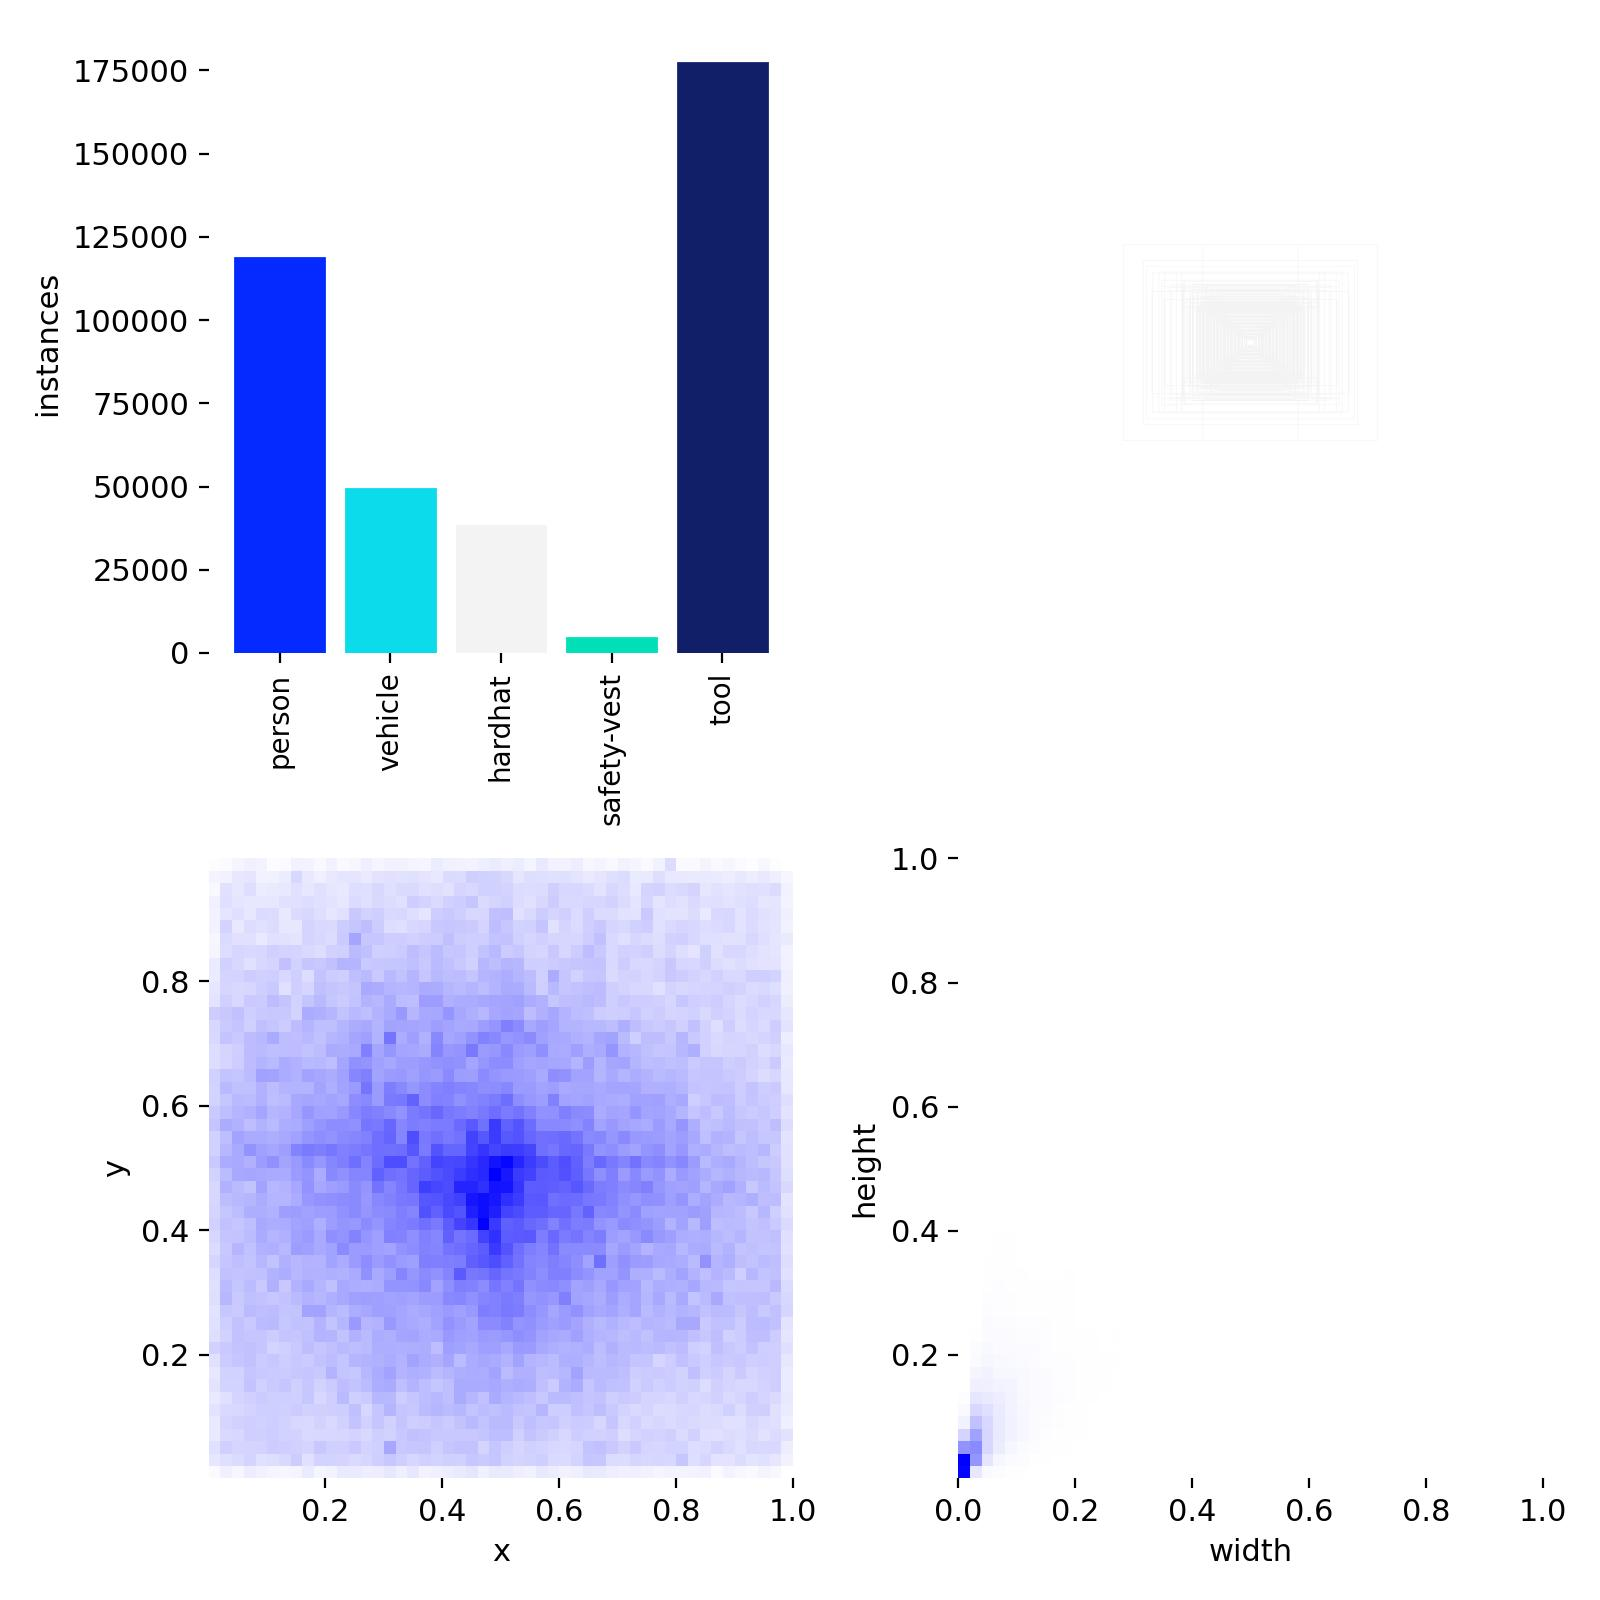
\includegraphics[width=\textwidth]{labels_pgie.jpg}
    \end{column}
    \begin{column}{0.37\textwidth}
      \textbf{5 classes:}
      \vspace{2mm}
      \begin{itemize}\small
        \item Person, Vehicle, Hardhat,\\Safety Vest, Tool
        \vspace{2mm}
        \item Classe \textit{Person} predominante\\--- reflete cenarios reais
        \vspace{2mm}
        \item Desbalanceamento natural mitigado via \textit{data augmentation}
      \end{itemize}

      \vspace{3mm}

      \begin{block}{\footnotesize Distribuicao Espacial}
        \footnotesize
        Concentracao central com dispersao uniforme --- boa cobertura do campo visual.
      \end{block}
    \end{column}
  \end{columns}
  \vfill
\end{frame}

% --- Slide: Distribuicao SGIEs ---
\begin{frame}{Distribuicao de Classes --- SGIEs}
  \vfill
  \begin{columns}[c]
    \begin{column}{0.5\textwidth}
      \centering
      {\footnotesize\textbf{SGIE-Ferramentas} (23 classes)}\\[2mm]
      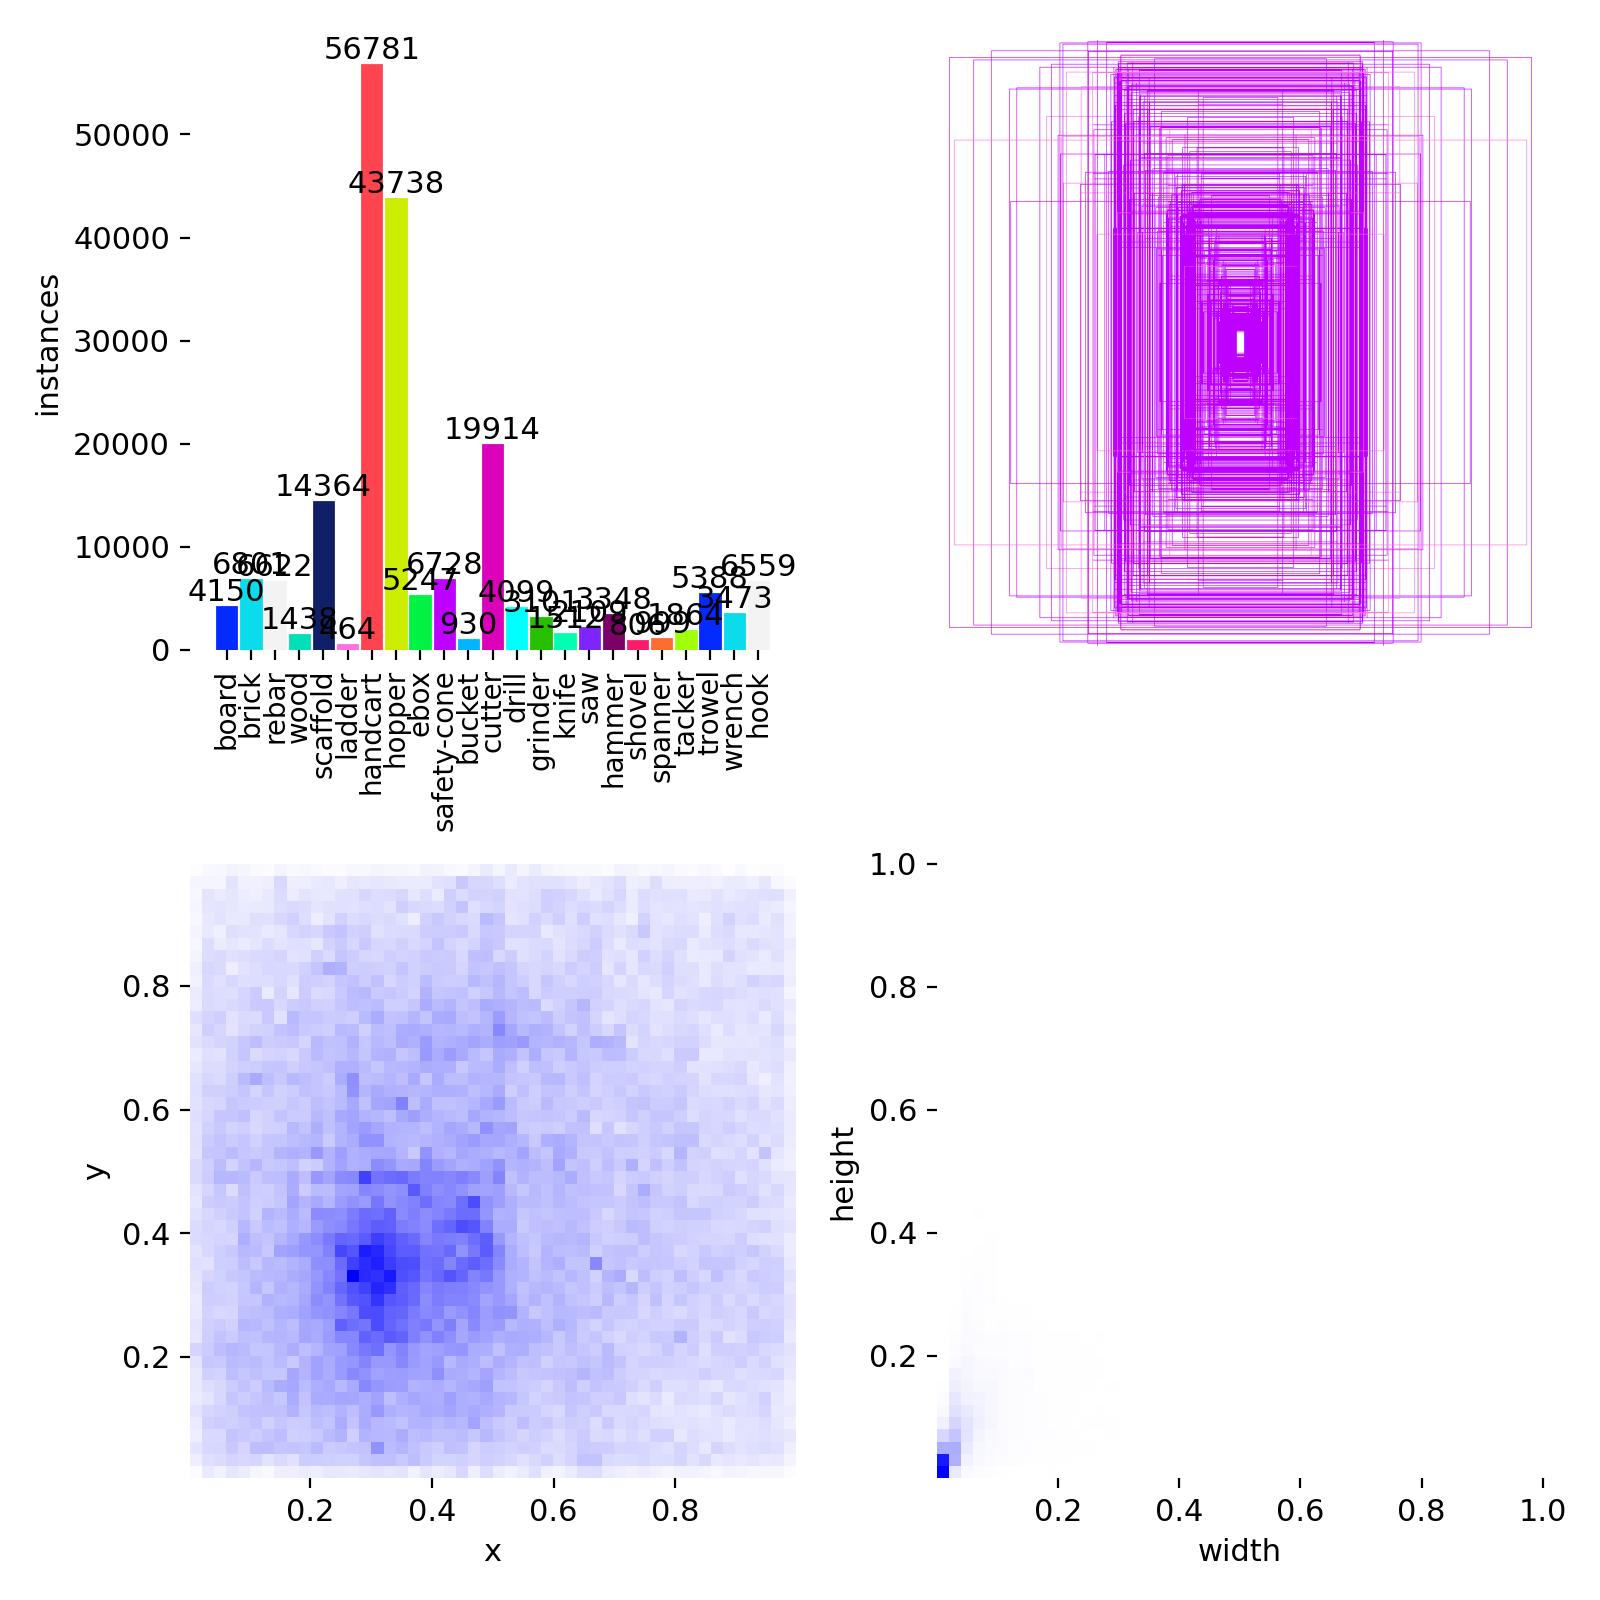
\includegraphics[width=\textwidth]{labels_sgie_equipment.jpg}

      \vspace{1mm}
      {\tiny Desbalanceamento significativo entre categorias}
    \end{column}
    \begin{column}{0.5\textwidth}
      \centering
      {\footnotesize\textbf{SGIE-Maquinario} (9 classes)}\\[2mm]
      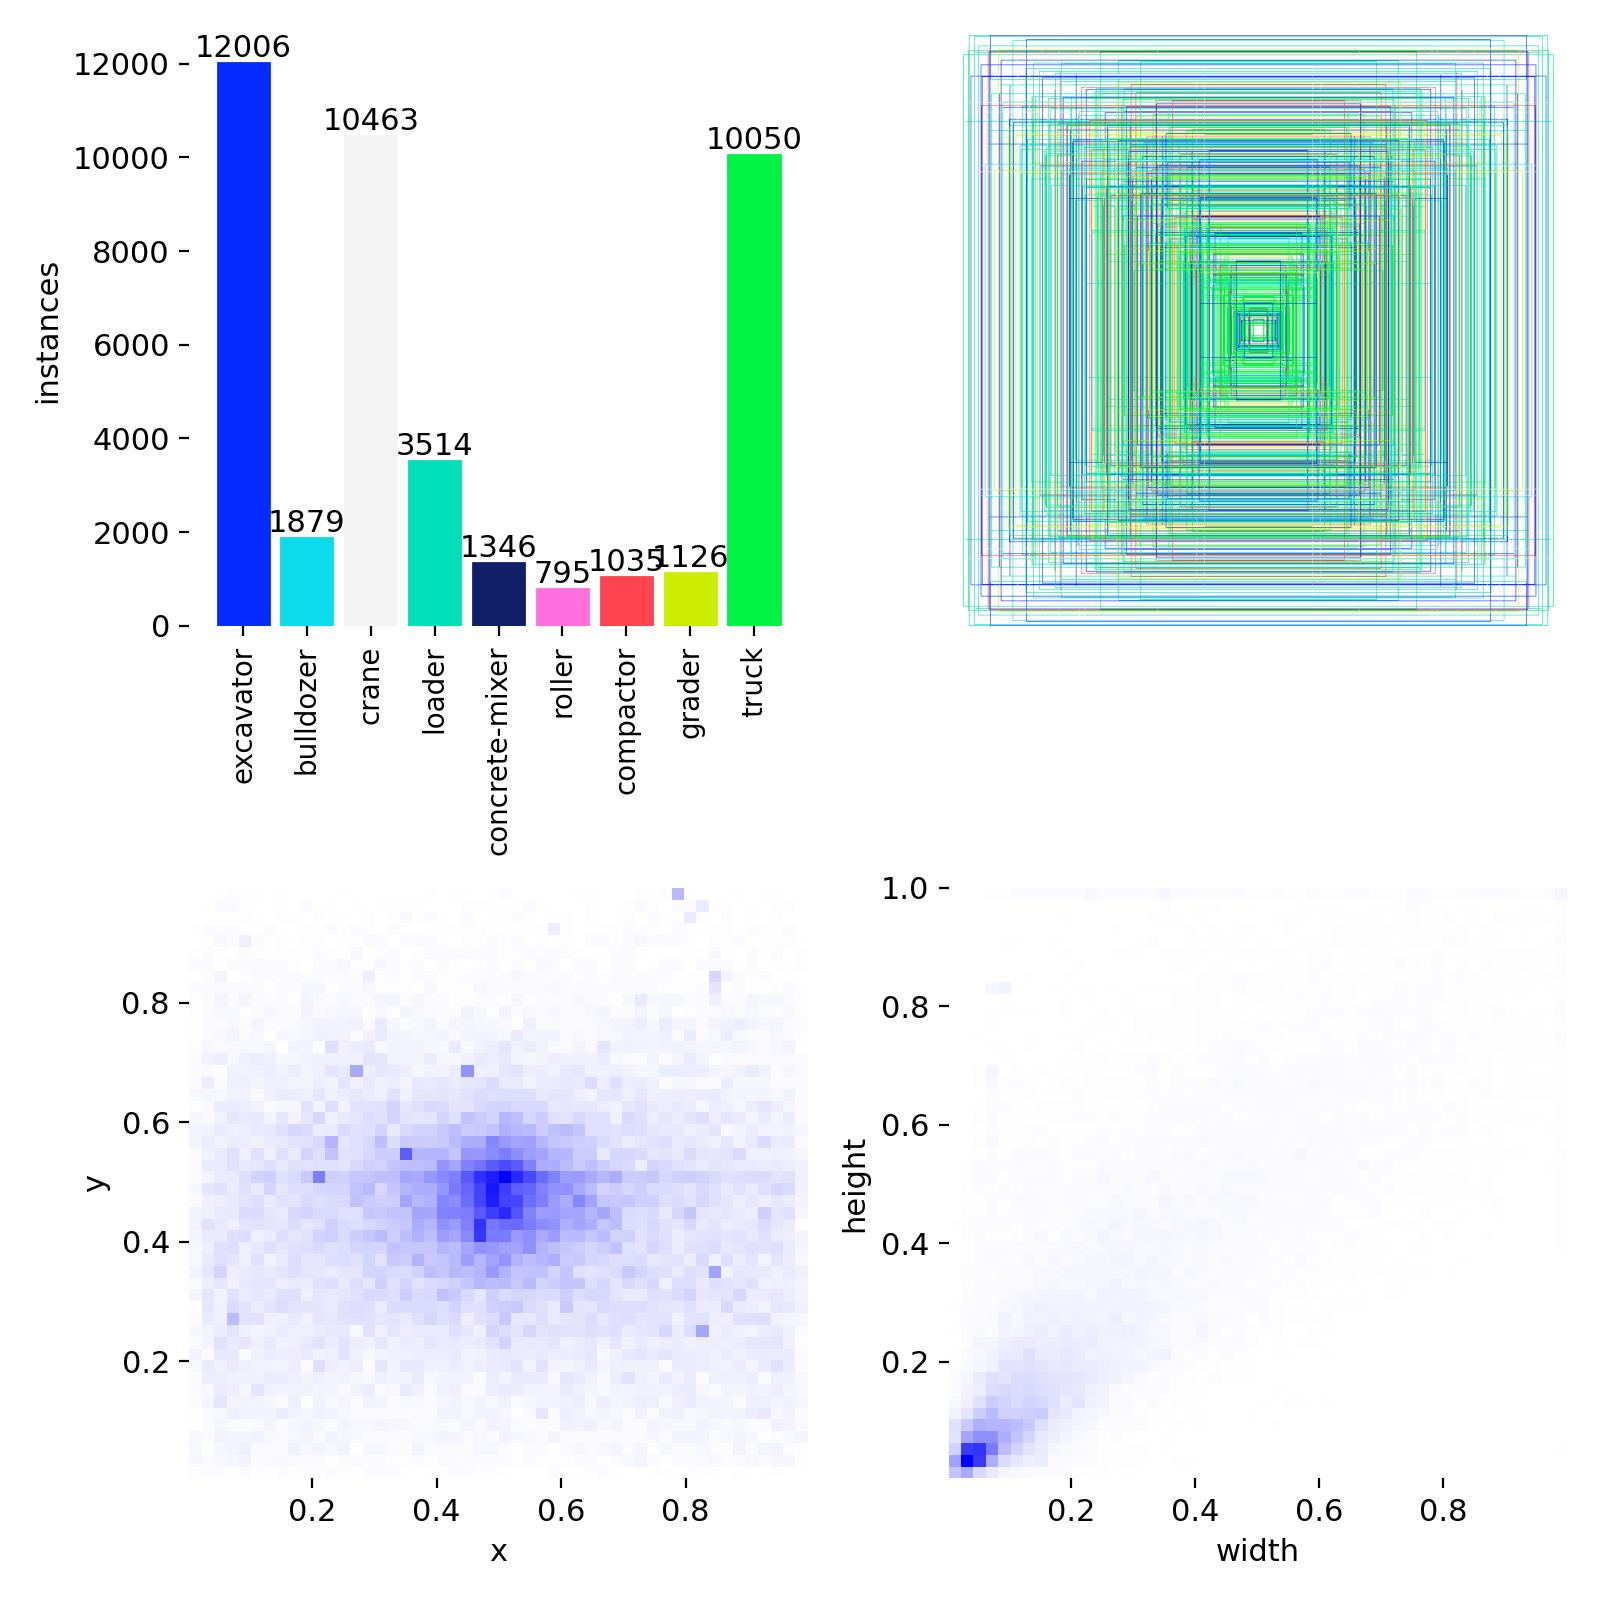
\includegraphics[width=\textwidth]{labels_sgie_machinery.jpg}

      \vspace{1mm}
      {\tiny Distribuicao mais equilibrada entre as classes}
    \end{column}
  \end{columns}

  \vspace{3mm}

  \begin{block}{}
    \centering\footnotesize
    O SGIE-EPI (14 classes) utiliza datasets especializados (SHWD, GDUT-HWD, PPE Detection)
    com foco em presenca/ausencia de EPIs --- distribuicao controlada por par positivo/negativo.
  \end{block}
  \vfill
\end{frame}

% --- Slide: Data Augmentation ---
\begin{frame}{Data Augmentation}
  \vfill
  \begin{columns}[c]
    \begin{column}{0.57\textwidth}
      \centering
      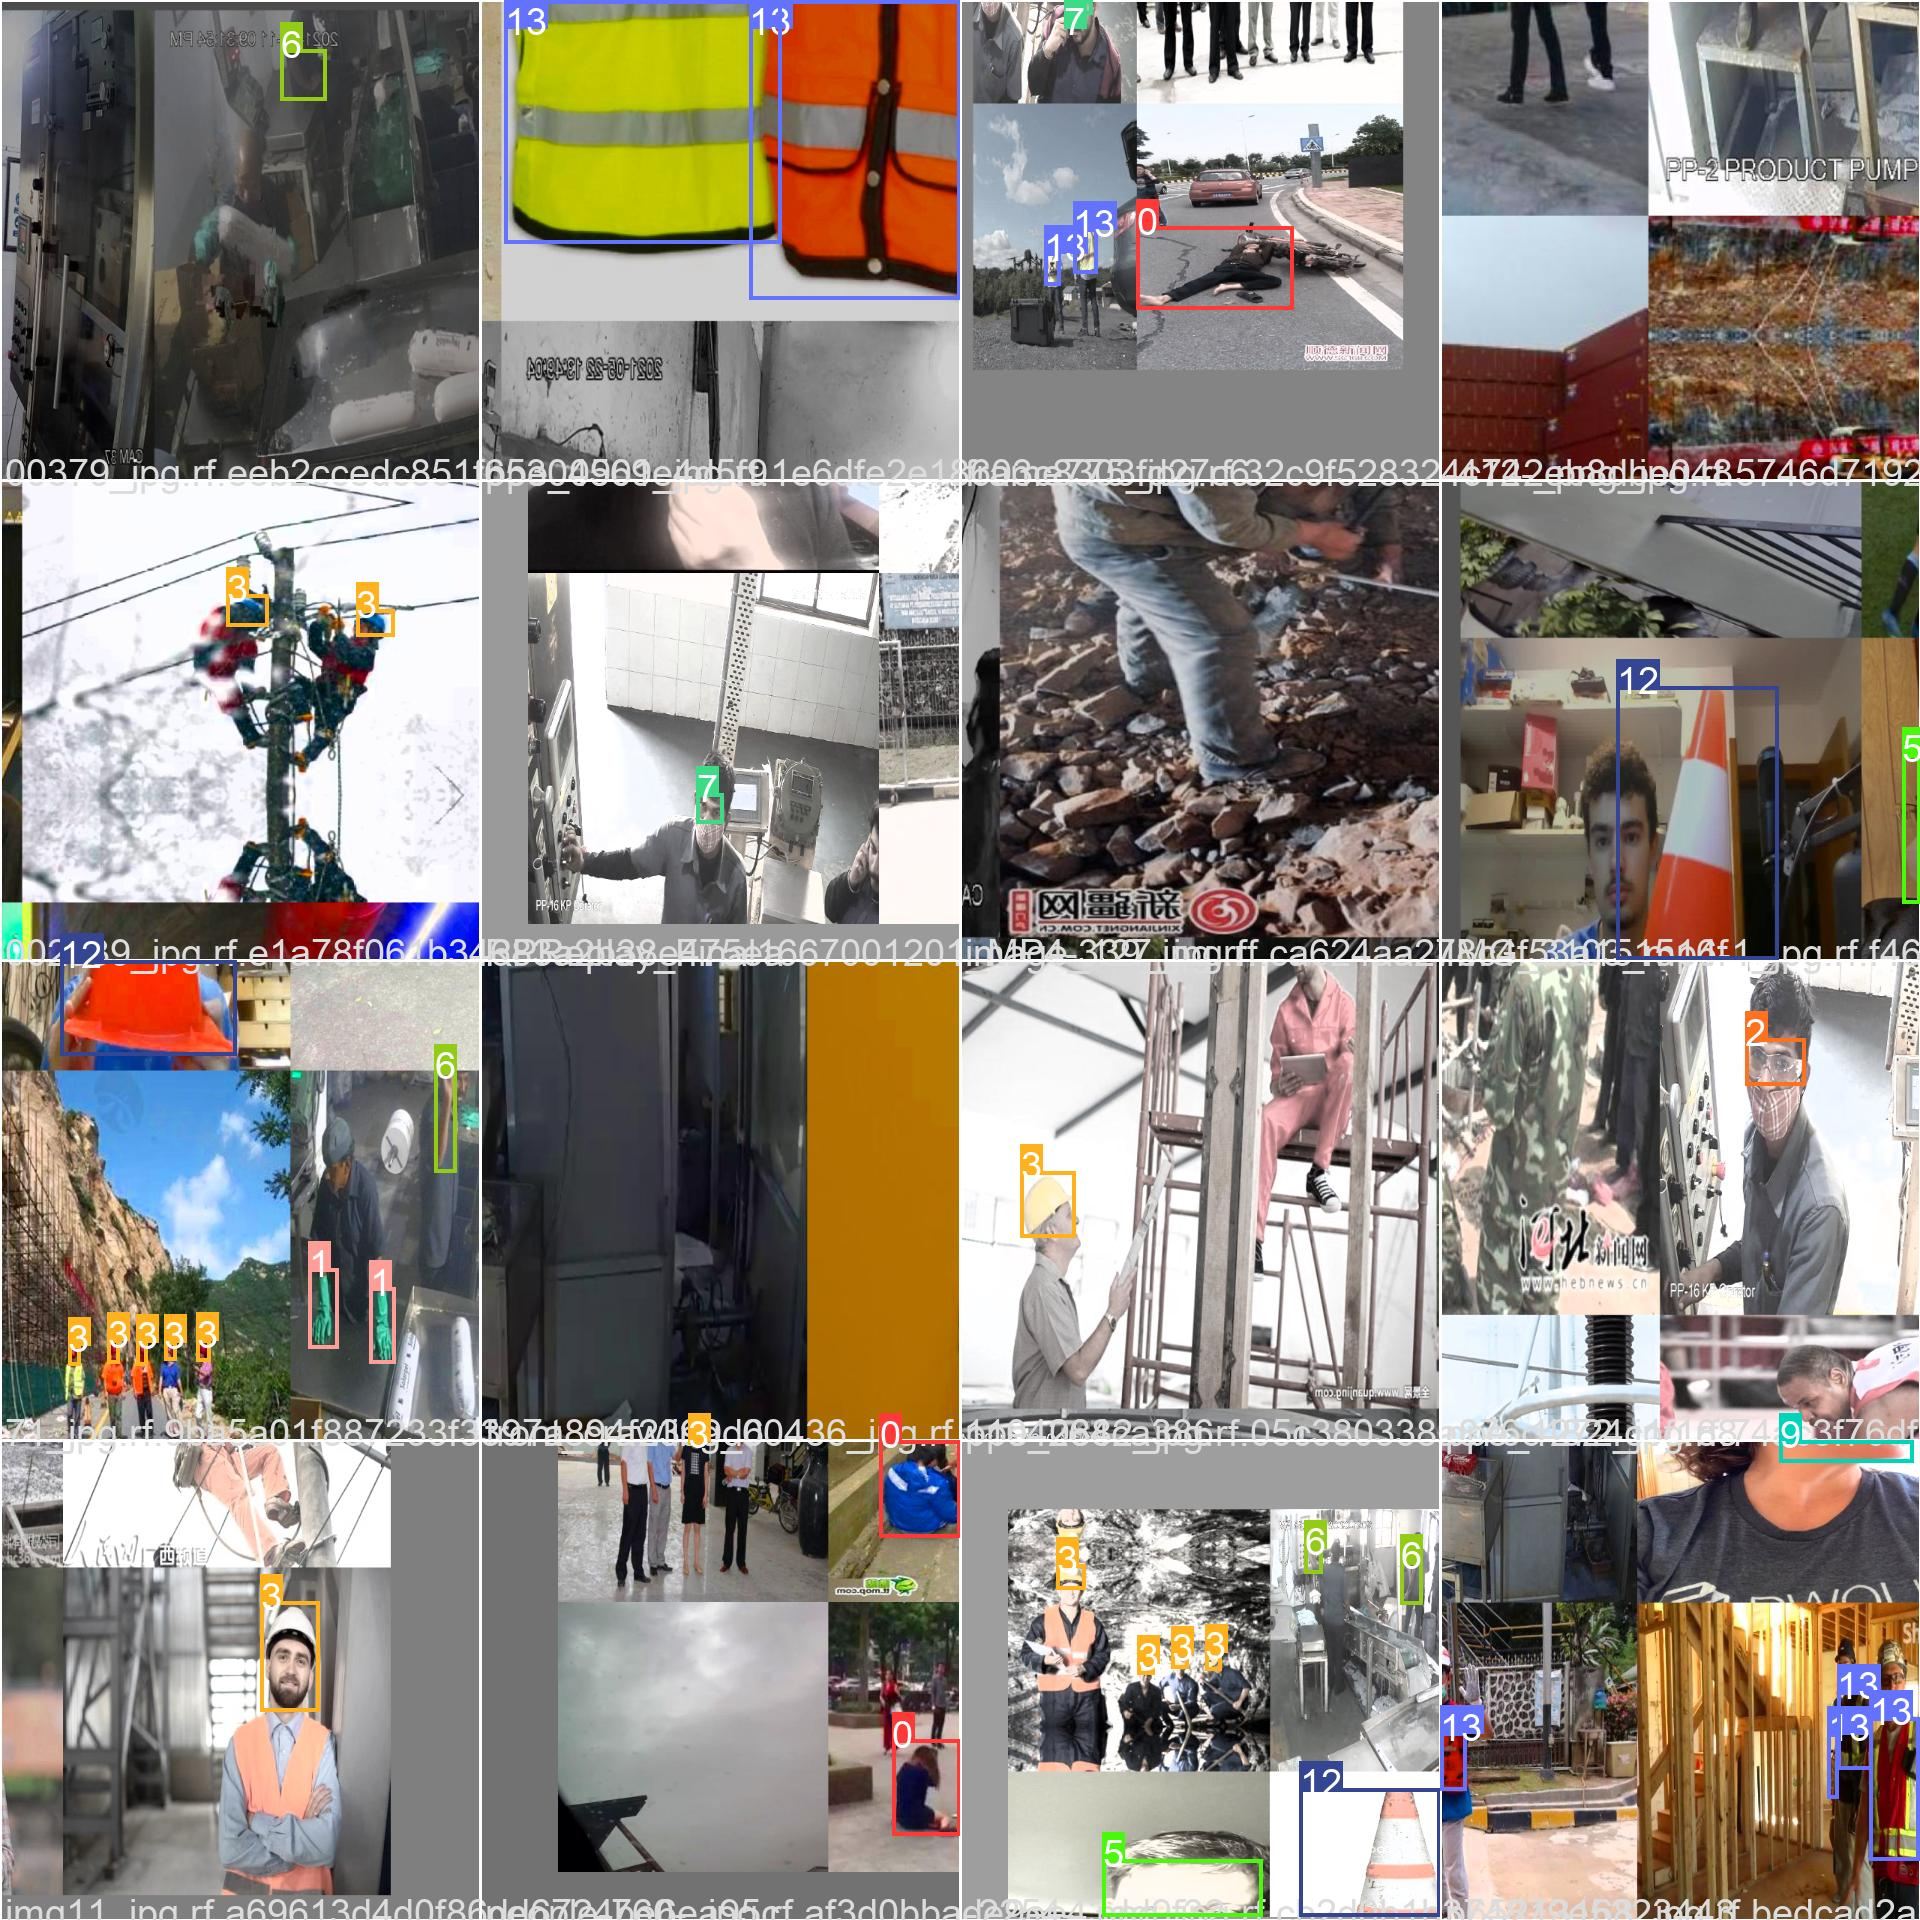
\includegraphics[width=\textwidth]{train_batch0.jpg}\\[1mm]
      {\tiny Amostra de batch de treinamento com augmentations aplicadas}
    \end{column}
    \begin{column}{0.40\textwidth}
      \textbf{Tecnicas e propositos:}
      \vspace{2mm}
      \begin{itemize}\small
        \item \textbf{Mosaic} (p=1.0)\\
          {\scriptsize Multi-escala, contexto variado}
        \vspace{2mm}
        \item \textbf{Flip horizontal} (p=0.5)\\
          {\scriptsize Invariancia a orientacao}
        \vspace{2mm}
        \item \textbf{Escala} (0.5x--1.5x)\\
          {\scriptsize Robustez a tamanhos variados}
        \vspace{2mm}
        \item \textbf{HSV} (h=0.015, s=0.7, v=0.4)\\
          {\scriptsize Invariancia a iluminacao}
        \vspace{2mm}
        \item \textbf{Translacao} (10\%)\\
          {\scriptsize Variacao de posicao}
      \end{itemize}
    \end{column}
  \end{columns}
  \vfill
\end{frame}

% --- Slide: Hiperparametros de Treinamento ---
\begin{frame}{Treinamento --- Hiperparametros}
  \vfill
  \begin{center}
    \small
    \renewcommand{\arraystretch}{1.25}
    \begin{tabular}{@{}lcc@{}}
      \toprule
      \textbf{Parametro} & \textbf{PGIE} & \textbf{SGIEs} \\
      \midrule
      \rowcolor{bgbox}
      Modelo base & YOLOv8m & YOLOv8s \\
      Resolucao & $640 \times 640$ & $320 \times 320$ \\
      \rowcolor{bgbox}
      Batch size & 16 & 32 \\
      Epocas maximas & 300 & 200 \\
      \rowcolor{bgbox}
      Otimizador & SGD & SGD \\
      LR inicial ($lr_0$) & 0,01 & 0,01 \\
      \rowcolor{bgbox}
      LR final ($lr_f$) & 0,01 & 0,01 \\
      Momentum & 0,937 & 0,937 \\
      \rowcolor{bgbox}
      Weight decay & 0,0005 & 0,0005 \\
      Warmup epochs & 3,0 & 3,0 \\
      \rowcolor{bgbox}
      Early stopping & 50 epocas & 30 epocas \\
      \bottomrule
    \end{tabular}
  \end{center}

  \vspace{3mm}

  \begin{columns}[c]
    \begin{column}{0.48\textwidth}
      \begin{block}{\footnotesize Funcao de Perda}
        \footnotesize
        $\mathcal{L} = \lambda_{box}\mathcal{L}_{box} + \lambda_{dfl}\mathcal{L}_{dfl} + \lambda_{cls}\mathcal{L}_{cls}$\\[1mm]
        {\scriptsize CIoU + Distribution Focal + BCE}
      \end{block}
    \end{column}
    \begin{column}{0.48\textwidth}
      \begin{block}{\footnotesize Ambiente}
        \footnotesize
        RTX 4070 (12\,GB), PyTorch 2.0\\
        Ultralytics YOLOv8 v8.0
      \end{block}
    \end{column}
  \end{columns}
  \vfill
\end{frame}

% --- Slide: Pipeline de Otimizacao ---
\begin{frame}{Pipeline de Otimizacao para Borda}
  \vfill
  \begin{center}
    \resizebox{0.95\textwidth}{!}{%
    \begin{tikzpicture}[node distance=16mm]
      \node[inputblock, minimum width=28mm, minimum height=14mm]
        (pt) {\textbf{PyTorch}\\(.pt)};
      \node[backboneblock, right=of pt, minimum width=28mm, minimum height=14mm]
        (onnx) {\textbf{ONNX}\\(.onnx)};
      \node[detectionblock, right=of onnx, minimum width=32mm, minimum height=14mm]
        (trt) {\textbf{TensorRT}\\FP16 (.engine)};
      \node[outputblock, right=of trt, minimum width=28mm, minimum height=14mm]
        (ds) {\textbf{DeepStream}\\Inferencia};

      \draw[arrow] (pt) -- node[above, font=\scriptsize\bfseries] {export} (onnx);
      \draw[arrow] (onnx) -- node[above, font=\scriptsize\bfseries] {otimizacao} (trt);
      \draw[arrow] (trt) -- node[above, font=\scriptsize\bfseries] {deploy} (ds);

      % Annotations below
      \node[below=5mm of pt, font=\tiny, align=center, text=sublabelcolor]
        {Treinamento\\GPU desktop};
      \node[below=5mm of onnx, font=\tiny, align=center, text=sublabelcolor]
        {Formato\\intermediario};
      \node[below=5mm of trt, font=\tiny, align=center, text=sublabelcolor]
        {Quantizacao FP16\\Fusao de camadas};
      \node[below=5mm of ds, font=\tiny, align=center, text=sublabelcolor]
        {Jetson AGX Xavier\\tempo real};
    \end{tikzpicture}
    }
  \end{center}

  \vspace{5mm}

  \begin{columns}[c]
    \begin{column}{0.48\textwidth}
      \begin{block}{\footnotesize Otimizacoes TensorRT}
        \begin{itemize}\scriptsize
          \item \textbf{Quantizacao FP16}: speedup ${\sim}$1.5--2x
          \item \textbf{Fusao de camadas}: Conv+BN+ReLU
          \item \textbf{Selecao de kernels}: otimizados p/ GPU alvo
        \end{itemize}
      \end{block}
    \end{column}
    \begin{column}{0.48\textwidth}
      \begin{block}{\footnotesize Conversao no Dispositivo}
        \begin{itemize}\scriptsize
          \item Compilado \textbf{diretamente no Jetson}
          \item Garante otimizacao especifica p/ hw
          \item Engine nao portavel entre GPUs
        \end{itemize}
      \end{block}
    \end{column}
  \end{columns}
  \vfill
\end{frame}

% ============================================================================
% CAPITULO 5 - IMPLEMENTACAO
% ============================================================================

\section{Implementação}

% --- Slide 19: Arquitetura Alto Nível ---
\begin{frame}{Arquitetura de Alto N\'{i}vel}
  \vspace{-2mm}
  \centering
  {\small Fluxo de v\'{i}deo processado pelo pipeline DeepStream no Jetson AGX Xavier.}

  \vspace{2mm}

  \begin{center}
    \resizebox{0.95\textwidth}{!}{%
    \begin{tikzpicture}[
      node distance=7mm,
      mainblock/.style={
        rectangle, rounded corners=4pt,
        minimum width=22mm, minimum height=13mm,
        align=center, font=\small\sffamily\bfseries,
        text=white, draw=none
      },
      sgieblock/.style={
        rectangle, rounded corners=3pt,
        minimum width=21mm, minimum height=11mm,
        align=center, font=\footnotesize\sffamily\bfseries,
        text=white, draw=none
      },
      arr/.style={-{Latex[length=2mm,width=1.5mm]}, thick, draw=arrowcolor},
    ]
      % Row 1: Input pipeline (left to right)
      \node[mainblock, fill=inputcolor] (cam) {C\^{a}mera\\{\tiny RTSP 1080p}};
      \node[mainblock, fill=backbonecolor, right=of cam] (dec) {NVDEC\\{\tiny Decode HW}};
      \node[mainblock, fill=cspcolor, right=of dec] (mux) {Streammux\\{\tiny Batching}};
      \node[mainblock, fill=detectioncolor, right=of mux] (pgie) {PGIE\\{\tiny YOLOv8m, 5\,cls}};
      \node[mainblock, fill=neckcolor, right=of pgie] (trk) {Tracker\\{\tiny NvDCF}};

      % Row 2: SGIEs + Output (right to left)
      \node[sgieblock, fill=headcolor, below=14mm of pgie, xshift=8mm] (sgie1) {SGIE-EPI\\{\tiny 14 cls}};
      \node[sgieblock, fill=headcolor, left=5mm of sgie1] (sgie2) {SGIE-Maq\\{\tiny 9 cls}};
      \node[sgieblock, fill=headcolor, right=5mm of sgie1] (sgie3) {SGIE-Fer\\{\tiny 23 cls}};
      \node[mainblock, fill=outputcolor, right=10mm of sgie3] (osd) {OSD\\{\tiny Overlay}};
      \node[mainblock, fill=skipcolor!80, left=10mm of sgie2] (sink) {Sa\'{i}da\\{\tiny Display}};

      % Arrows Row 1
      \draw[arr] (cam) -- (dec);
      \draw[arr] (dec) -- (mux);
      \draw[arr] (mux) -- (pgie);
      \draw[arr] (pgie) -- (trk);

      % Arrow down from tracker to SGIEs
      \draw[arr] (trk.south) -- ++(0,-4mm) -| (sgie1.north);
      \draw[arr] (trk.south) -- ++(0,-4mm) -| (sgie2.north);
      \draw[arr] (trk.south) -- ++(0,-4mm) -| (sgie3.north);

      % SGIEs to OSD and Sink
      \draw[arr] (sgie3.east) -- (osd.west);
      \draw[arr] (sgie2.west) -- (sink.east);

      % Brace for GPU acceleration
      \draw[thick, skipcolor, decorate, decoration={brace, amplitude=3pt, raise=3pt}]
        (mux.north west) -- (trk.north east)
        node[midway, above=6pt, font=\scriptsize\sffamily\bfseries, text=skipcolor]
        {Aceleração GPU / TensorRT FP16};
    \end{tikzpicture}
    }
  \end{center}

  \vspace{2mm}

  \begin{beamercolorbox}[wd=\textwidth, rounded=true, shadow=false]{block body}
    \centering
    {\footnotesize\color{stagecolor}%
      Cascata PGIE $\to$ 3 SGIEs com roteamento por classe --- \textbf{20 FPS} / \textbf{58\,ms} de lat\^{e}ncia.}
  \end{beamercolorbox}
  \vfill
\end{frame}

% --- Slide 20: Pipeline DeepStream (mesclado com detalhado) ---
\begin{frame}{Pipeline DeepStream}
  \smallskip
  \centering
  {\small Pipeline GStreamer com aceleração por hardware --- captura $\to$ inferência em cascata $\to$ alertas.}

  \vspace{3mm}

  \begin{center}
    \resizebox{0.98\textwidth}{!}{% ============================================================================
% Diagrama do Pipeline GStreamer/DeepStream
% Para inclusao na dissertacao de mestrado - PPGC/UFRGS
% ============================================================================
% Uso: % ============================================================================
% Diagrama do Pipeline GStreamer/DeepStream
% Para inclusao na dissertacao de mestrado - PPGC/UFRGS
% ============================================================================
% Uso: \input{figuras/diagrama_pipeline.tex}
% Requer: \usepackage{tikz}
%         \usetikzlibrary{shapes.geometric, arrows.meta, positioning, fit, calc}
% ============================================================================

\begin{tikzpicture}[
    % Definicao de estilos
    node distance=0.6cm and 0.8cm,
    % Estilo base para blocos do pipeline (sem parametro #1)
    blockbase/.style={
        rectangle,
        line width=1pt,
        minimum width=2.2cm,
        minimum height=1.2cm,
        align=center,
        font=\small\sffamily,
        rounded corners=2pt
    },
    % Estilo para setas
    arrow/.style={
        ->,
        >=Stealth,
        line width=0.8pt,
        draw=black!70
    },
    % Estilo para grupo/container
    containerbase/.style={
        rectangle,
        dashed,
        line width=0.8pt,
        rounded corners=4pt,
        inner sep=8pt
    },
]

% ============================================================================
% Primeira linha: Source -> Decoder -> Streammux
% ============================================================================

% Source
\node[blockbase, draw=teal!80!black, fill=teal!80!black!10] (source) {
    \textbf{Source}\\[2pt]
    Camera/Arquivo
};
\node[font=\scriptsize\ttfamily, text=teal!80!black!80, below=0.1cm of source] {\textit{nvv4l2camerasrc}};
\node[font=\scriptsize\ttfamily, text=teal!80!black!80, below=0.35cm of source] {\textit{filesrc}};

% Decoder
\node[blockbase, draw=cyan!70!black, fill=cyan!70!black!10, right=of source] (decoder) {
    \textbf{Decoder}\\[2pt]
    Decodificacao
};
\node[font=\scriptsize\ttfamily, text=cyan!70!black!80, below=0.1cm of decoder] {\textit{nvv4l2decoder}};

% Streammux
\node[blockbase, draw=blue!70!black, fill=blue!70!black!10, right=of decoder] (streammux) {
    \textbf{Streammux}\\[2pt]
    Batching
};
\node[font=\scriptsize\ttfamily, text=blue!70!black!80, below=0.1cm of streammux] {\textit{nvstreammux}};

% ============================================================================
% Segunda linha: PGIE
% ============================================================================

% PGIE
\node[blockbase, draw=purple!70!black, fill=purple!70!black!10, right=of streammux] (pgie) {
    \textbf{PGIE}\\[2pt]
    Primary Inference
};
\node[font=\scriptsize\ttfamily, text=purple!70!black!80, below=0.1cm of pgie] {\textit{nvinfer}};

% ============================================================================
% Tracker
% ============================================================================

% Tracker
\node[blockbase, draw=violet!70!black, fill=violet!70!black!10, right=of pgie] (tracker) {
    \textbf{Tracker}\\[2pt]
    Object Tracking
};
\node[font=\scriptsize\ttfamily, text=violet!70!black!80, below=0.1cm of tracker] {\textit{nvtracker}};

% ============================================================================
% Container para SGIEs
% ============================================================================

% SGIE-1
\node[blockbase, draw=orange!70!black, fill=orange!70!black!10, right=1.5cm of tracker, yshift=1.2cm] (sgie1) {
    \textbf{SGIE-1}\\[2pt]
    EPI Detection
};
\node[font=\scriptsize\ttfamily, text=orange!70!black!80, below=0.1cm of sgie1] {\textit{nvinfer}};

% SGIE-2
\node[blockbase, draw=orange!70!black, fill=orange!70!black!10, right=1.5cm of tracker] (sgie2) {
    \textbf{SGIE-2}\\[2pt]
    Machinery ID
};
\node[font=\scriptsize\ttfamily, text=orange!70!black!80, below=0.1cm of sgie2] {\textit{nvinfer}};

% SGIE-3
\node[blockbase, draw=orange!70!black, fill=orange!70!black!10, right=1.5cm of tracker, yshift=-1.2cm] (sgie3) {
    \textbf{SGIE-3}\\[2pt]
    Tools Detection
};
\node[font=\scriptsize\ttfamily, text=orange!70!black!80, below=0.1cm of sgie3] {\textit{nvinfer}};

% Container para SGIEs
\node[containerbase, draw=orange!60, fill=orange!5, fit=(sgie1)(sgie2)(sgie3), label={[font=\small\sffamily,orange!70!black]above:Secondary Inference Engines}] (sgiegroup) {};

% ============================================================================
% OSD e Sink
% ============================================================================

% OSD
\node[blockbase, draw=green!60!black, fill=green!60!black!10, right=1.5cm of sgie2] (osd) {
    \textbf{OSD}\\[2pt]
    On-Screen Display
};
\node[font=\scriptsize\ttfamily, text=green!60!black!80, below=0.1cm of osd] {\textit{nvdsosd}};

% Sink
\node[blockbase, draw=red!60!black, fill=red!60!black!10, right=of osd] (sink) {
    \textbf{Sink}\\[2pt]
    Output
};
\node[font=\scriptsize\ttfamily, text=red!60!black!80, below=0.1cm of sink] {\textit{nveglglessink}};
\node[font=\scriptsize\ttfamily, text=red!60!black!80, below=0.35cm of sink] {\textit{filesink}};

% ============================================================================
% Setas de conexao
% ============================================================================

% Fluxo principal
\draw[arrow] (source) -- (decoder);
\draw[arrow] (decoder) -- (streammux);
\draw[arrow] (streammux) -- (pgie);
\draw[arrow] (pgie) -- (tracker);

% Tracker para SGIEs
\draw[arrow] (tracker.east) -- ++(0.3,0) |- (sgie1.west);
\draw[arrow] (tracker.east) -- (sgie2.west);
\draw[arrow] (tracker.east) -- ++(0.3,0) |- (sgie3.west);

% SGIEs para OSD
\draw[arrow] (sgie1.east) -| ($(osd.west)+(-0.3,0)$) -- (osd.west);
\draw[arrow] (sgie2.east) -- (osd.west);
\draw[arrow] (sgie3.east) -| ($(osd.west)+(-0.3,0)$) -- (osd.west);

% OSD para Sink
\draw[arrow] (osd) -- (sink);

% ============================================================================
% Legenda de fluxo de dados
% ============================================================================

% Indicador de direcao do fluxo
\node[font=\small\sffamily, text=black!60, below=2.5cm of streammux] (flowlabel) {Fluxo de dados $\longrightarrow$};

\end{tikzpicture}

% Requer: \usepackage{tikz}
%         \usetikzlibrary{shapes.geometric, arrows.meta, positioning, fit, calc}
% ============================================================================

\begin{tikzpicture}[
    % Definicao de estilos
    node distance=0.6cm and 0.8cm,
    % Estilo base para blocos do pipeline (sem parametro #1)
    blockbase/.style={
        rectangle,
        line width=1pt,
        minimum width=2.2cm,
        minimum height=1.2cm,
        align=center,
        font=\small\sffamily,
        rounded corners=2pt
    },
    % Estilo para setas
    arrow/.style={
        ->,
        >=Stealth,
        line width=0.8pt,
        draw=black!70
    },
    % Estilo para grupo/container
    containerbase/.style={
        rectangle,
        dashed,
        line width=0.8pt,
        rounded corners=4pt,
        inner sep=8pt
    },
]

% ============================================================================
% Primeira linha: Source -> Decoder -> Streammux
% ============================================================================

% Source
\node[blockbase, draw=teal!80!black, fill=teal!80!black!10] (source) {
    \textbf{Source}\\[2pt]
    Camera/Arquivo
};
\node[font=\scriptsize\ttfamily, text=teal!80!black!80, below=0.1cm of source] {\textit{nvv4l2camerasrc}};
\node[font=\scriptsize\ttfamily, text=teal!80!black!80, below=0.35cm of source] {\textit{filesrc}};

% Decoder
\node[blockbase, draw=cyan!70!black, fill=cyan!70!black!10, right=of source] (decoder) {
    \textbf{Decoder}\\[2pt]
    Decodificacao
};
\node[font=\scriptsize\ttfamily, text=cyan!70!black!80, below=0.1cm of decoder] {\textit{nvv4l2decoder}};

% Streammux
\node[blockbase, draw=blue!70!black, fill=blue!70!black!10, right=of decoder] (streammux) {
    \textbf{Streammux}\\[2pt]
    Batching
};
\node[font=\scriptsize\ttfamily, text=blue!70!black!80, below=0.1cm of streammux] {\textit{nvstreammux}};

% ============================================================================
% Segunda linha: PGIE
% ============================================================================

% PGIE
\node[blockbase, draw=purple!70!black, fill=purple!70!black!10, right=of streammux] (pgie) {
    \textbf{PGIE}\\[2pt]
    Primary Inference
};
\node[font=\scriptsize\ttfamily, text=purple!70!black!80, below=0.1cm of pgie] {\textit{nvinfer}};

% ============================================================================
% Tracker
% ============================================================================

% Tracker
\node[blockbase, draw=violet!70!black, fill=violet!70!black!10, right=of pgie] (tracker) {
    \textbf{Tracker}\\[2pt]
    Object Tracking
};
\node[font=\scriptsize\ttfamily, text=violet!70!black!80, below=0.1cm of tracker] {\textit{nvtracker}};

% ============================================================================
% Container para SGIEs
% ============================================================================

% SGIE-1
\node[blockbase, draw=orange!70!black, fill=orange!70!black!10, right=1.5cm of tracker, yshift=1.2cm] (sgie1) {
    \textbf{SGIE-1}\\[2pt]
    EPI Detection
};
\node[font=\scriptsize\ttfamily, text=orange!70!black!80, below=0.1cm of sgie1] {\textit{nvinfer}};

% SGIE-2
\node[blockbase, draw=orange!70!black, fill=orange!70!black!10, right=1.5cm of tracker] (sgie2) {
    \textbf{SGIE-2}\\[2pt]
    Machinery ID
};
\node[font=\scriptsize\ttfamily, text=orange!70!black!80, below=0.1cm of sgie2] {\textit{nvinfer}};

% SGIE-3
\node[blockbase, draw=orange!70!black, fill=orange!70!black!10, right=1.5cm of tracker, yshift=-1.2cm] (sgie3) {
    \textbf{SGIE-3}\\[2pt]
    Tools Detection
};
\node[font=\scriptsize\ttfamily, text=orange!70!black!80, below=0.1cm of sgie3] {\textit{nvinfer}};

% Container para SGIEs
\node[containerbase, draw=orange!60, fill=orange!5, fit=(sgie1)(sgie2)(sgie3), label={[font=\small\sffamily,orange!70!black]above:Secondary Inference Engines}] (sgiegroup) {};

% ============================================================================
% OSD e Sink
% ============================================================================

% OSD
\node[blockbase, draw=green!60!black, fill=green!60!black!10, right=1.5cm of sgie2] (osd) {
    \textbf{OSD}\\[2pt]
    On-Screen Display
};
\node[font=\scriptsize\ttfamily, text=green!60!black!80, below=0.1cm of osd] {\textit{nvdsosd}};

% Sink
\node[blockbase, draw=red!60!black, fill=red!60!black!10, right=of osd] (sink) {
    \textbf{Sink}\\[2pt]
    Output
};
\node[font=\scriptsize\ttfamily, text=red!60!black!80, below=0.1cm of sink] {\textit{nveglglessink}};
\node[font=\scriptsize\ttfamily, text=red!60!black!80, below=0.35cm of sink] {\textit{filesink}};

% ============================================================================
% Setas de conexao
% ============================================================================

% Fluxo principal
\draw[arrow] (source) -- (decoder);
\draw[arrow] (decoder) -- (streammux);
\draw[arrow] (streammux) -- (pgie);
\draw[arrow] (pgie) -- (tracker);

% Tracker para SGIEs
\draw[arrow] (tracker.east) -- ++(0.3,0) |- (sgie1.west);
\draw[arrow] (tracker.east) -- (sgie2.west);
\draw[arrow] (tracker.east) -- ++(0.3,0) |- (sgie3.west);

% SGIEs para OSD
\draw[arrow] (sgie1.east) -| ($(osd.west)+(-0.3,0)$) -- (osd.west);
\draw[arrow] (sgie2.east) -- (osd.west);
\draw[arrow] (sgie3.east) -| ($(osd.west)+(-0.3,0)$) -- (osd.west);

% OSD para Sink
\draw[arrow] (osd) -- (sink);

% ============================================================================
% Legenda de fluxo de dados
% ============================================================================

% Indicador de direcao do fluxo
\node[font=\small\sffamily, text=black!60, below=2.5cm of streammux] (flowlabel) {Fluxo de dados $\longrightarrow$};

\end{tikzpicture}
}
  \end{center}

  \vspace{2mm}

  \begin{center}
    \scriptsize
    \renewcommand{\arraystretch}{1.1}
    \begin{tabular}{@{}p{0.15\textwidth}p{0.15\textwidth}p{0.15\textwidth}p{0.15\textwidth}p{0.15\textwidth}p{0.15\textwidth}@{}}
      \textcolor{teal!80!black}{\textbf{Source}} &
      \textcolor{cyan!70!black}{\textbf{Decoder}} &
      \textcolor{blue!70!black}{\textbf{Streammux}} &
      \textcolor{purple!70!black}{\textbf{PGIE}} &
      \textcolor{violet!70!black}{\textbf{Tracker}} &
      \textcolor{orange!70!black}{\textbf{SGIEs}} \\
      Captura RTSP &
      NVDEC (hw) &
      Batching &
      Detec\c{c}\~{a}o prim\'{a}ria &
      Rastreamento IDs &
      Classifica\c{c}\~{a}o fina \\
    \end{tabular}
  \end{center}

  \vspace{2mm}

  \begin{block}{}
    \centering\footnotesize
    Cada componente \'{e} um plugin GStreamer otimizado --- aceleração por \textbf{GPU/TensorRT} entre Streammux e SGIEs.
  \end{block}
  \vfill
\end{frame}

% --- Slide 22: Parser C++ Customizado (NOVO) ---
\begin{frame}{Parser C++ Customizado}
  \vspace{-2mm}
  \centering
  {\small Roteamento de detecções do PGIE para SGIEs especializados via ROI recortada.}

  \vspace{1mm}

  \begin{center}
  \resizebox{0.95\textwidth}{!}{%
  \begin{tikzpicture}[
    node distance=0.5cm and 1.0cm,
    pgiebox/.style={
      rectangle, draw=purple!70!black, fill=purple!10,
      minimum width=2.4cm, minimum height=0.8cm,
      align=center, font=\footnotesize\sffamily, rounded corners=3pt, line width=0.8pt
    },
    sgiebox/.style={
      rectangle, draw=orange!70!black, fill=orange!10,
      minimum width=2.2cm, minimum height=0.7cm,
      align=center, font=\footnotesize\sffamily, rounded corners=3pt, line width=0.8pt
    },
    routebox/.style={
      rectangle, draw=labelcolor, fill=bgbox,
      minimum width=2.8cm, minimum height=0.6cm,
      align=center, font=\scriptsize\ttfamily, rounded corners=2pt
    },
    myarrow/.style={
      -{Latex[length=2mm,width=1.5mm]},
      line width=0.7pt, draw=arrowcolor
    }
  ]
    % PGIE
    \node[pgiebox] (pgie) {\textbf{PGIE}\\{\scriptsize 5 classes}};

    % Routing conditions
    \node[routebox, right=1.2cm of pgie, yshift=1.0cm] (r0) {class\_id == 0 (Person)};
    \node[routebox, right=1.2cm of pgie] (r1) {class\_id == 1 (Vehicle)};
    \node[routebox, right=1.2cm of pgie, yshift=-1.0cm] (r4) {class\_id == 4 (Tool)};

    % SGIEs
    \node[sgiebox, right=1.0cm of r0] (sgie1) {\textbf{SGIE-EPI}\\{\scriptsize 14 cls}};
    \node[sgiebox, right=1.0cm of r1] (sgie2) {\textbf{SGIE-Maq}\\{\scriptsize 9 cls}};
    \node[sgiebox, right=1.0cm of r4] (sgie3) {\textbf{SGIE-Fer}\\{\scriptsize 23 cls}};

    % Arrows PGIE -> routing
    \draw[myarrow] (pgie.east) -- ++(0.25,0) |- (r0.west);
    \draw[myarrow] (pgie.east) -- (r1.west);
    \draw[myarrow] (pgie.east) -- ++(0.25,0) |- (r4.west);

    % Arrows routing -> SGIEs
    \draw[myarrow, draw=detectioncolor] (r0.east) -- node[above, font=\tiny, text=detectioncolor] {crop} (sgie1.west);
    \draw[myarrow, draw=detectioncolor] (r1.east) -- node[above, font=\tiny, text=detectioncolor] {crop} (sgie2.west);
    \draw[myarrow, draw=detectioncolor] (r4.east) -- node[above, font=\tiny, text=detectioncolor] {crop} (sgie3.west);

  \end{tikzpicture}
  }
  \end{center}

  \vspace{1mm}

  \begin{columns}[t]
    \begin{column}{0.48\textwidth}
      \begin{block}{\scriptsize Função do Parser}
        \begin{itemize}\scriptsize
          \setlength{\itemsep}{0pt}
          \item Decodifica saída \textit{anchor-free} YOLOv8
          \item Filtragem por confiança + NMS
          \item Compilado como \texttt{.so} (C++)
        \end{itemize}
      \end{block}
    \end{column}
    \begin{column}{0.48\textwidth}
      \begin{block}{\scriptsize Roteamento}
        \begin{itemize}\scriptsize
          \setlength{\itemsep}{0pt}
          \item SGIE opera via \texttt{operate-on-class-ids}
          \item ROI recortada da bbox do PGIE
          \item Processam apenas regiões de interesse
        \end{itemize}
      \end{block}
    \end{column}
  \end{columns}
  \vfill
\end{frame}

% --- Slide 23: Software Stack (Layered TikZ) ---
\begin{frame}{Software Stack}
  \vspace{-2mm}
  \centering
  {\small Pilha de software otimizada para inferência em borda no Jetson AGX Xavier.}

  \vspace{1mm}

  \begin{center}
  \begin{tikzpicture}[
    layerbase/.style={
      rectangle,
      minimum width=10cm, minimum height=0.7cm,
      align=center, font=\footnotesize\sffamily, rounded corners=2pt,
      line width=0.8pt
    },
  ]
    % Layers from bottom to top (spacing 0.78cm)
    \node[layerbase, draw=buscolor!80!black, fill=buscolor!15] (hw) at (0,0) {\textbf{Hardware} --- Jetson AGX Xavier (512 CUDA, 32~GB)};
    \node[layerbase, draw=cpucolor!80!black, fill=cpucolor!15] (os) at (0,0.78) {\textbf{JetPack 5.1.2} --- Ubuntu 20.04 + drivers NVIDIA};
    \node[layerbase, draw=gpucolor!80!black, fill=gpucolor!15] (cuda) at (0,1.56) {\textbf{CUDA 11.4} + \textbf{cuDNN 8.6} --- Aceleração GPU};
    \node[layerbase, draw=memcolor!80!black, fill=memcolor!15] (trt) at (0,2.34) {\textbf{TensorRT 8.5.2} --- Otimização FP16};
    \node[layerbase, draw=neckcolor!80!black, fill=neckcolor!15] (ds) at (0,3.12) {\textbf{DeepStream 6.2} + \textbf{GStreamer 1.16} --- Pipeline};
    \node[layerbase, draw=headcolor!80!black, fill=headcolor!15] (app) at (0,3.90) {\textbf{Aplicação Python} + \textbf{Parser C++ (.so)}};

    % Side arrows
    \draw[-{Latex[length=2mm]}, line width=1.5pt, draw=arrowcolor]
      (-5.8,0) -- (-5.8,3.90) node[midway, rotate=90, above, font=\footnotesize\sffamily, text=arrowcolor] {Nível de abstração};

  \end{tikzpicture}
  \end{center}

  \vspace{1mm}

  \begin{center}
    \scriptsize
    \textcolor{labelcolor}{Modelos exportados em \textbf{FP16} via TensorRT --- speedup de \textbf{1,7$\times$} sobre FP32.}
  \end{center}

  \vfill
\end{frame}

% --- Slide 24: Deployment (NOVO) ---
\begin{frame}{Deployment na Borda}
  \vspace{-2mm}
  \centering
  {\small Aspectos práticos de implantação do sistema no Jetson AGX Xavier.}

  \vspace{1mm}

  \begin{columns}[t]
    \begin{column}{0.48\textwidth}
      \begin{block}{\scriptsize Configuração do Dispositivo}
        \begin{itemize}\scriptsize
          \setlength{\itemsep}{0pt}
          \item Modo de potência: \textbf{MAXN (30\,W)}
          \item 512 CUDA cores ativos
          \item 8 cores ARM v8.2 a 2,26 GHz
          \item 32 GB LPDDR4x compartilhada
        \end{itemize}
      \end{block}

      \begin{block}{\scriptsize Entrada de Vídeo}
        \begin{itemize}\scriptsize
          \setlength{\itemsep}{0pt}
          \item Stream \textbf{RTSP} via rede local
          \item Decodificação por \textbf{NVDEC} (hw)
          \item 1920$\times$1080 $\to$ 640$\times$640
        \end{itemize}
      \end{block}
    \end{column}

    \begin{column}{0.48\textwidth}
      \begin{block}{\scriptsize Saída e Visualização}
        \begin{itemize}\scriptsize
          \setlength{\itemsep}{0pt}
          \item Display local via \texttt{nveglglessink}
          \item Gravação via \texttt{filesink}
          \item Bboxes + labels + alertas EPI
        \end{itemize}
      \end{block}

      \begin{block}{\scriptsize Otimizações Aplicadas}
        \begin{itemize}\scriptsize
          \setlength{\itemsep}{0pt}
          \item Memória unificada CPU-GPU
          \item Batching de crops para SGIEs
          \item Pipeline assíncrono (GStreamer)
          \item Quantização FP16 em todos os modelos
        \end{itemize}
      \end{block}
    \end{column}
  \end{columns}

  \vfill

  \begin{center}
    \scriptsize
    \textcolor{labelcolor}{Pipeline completo: \textbf{20 FPS} / \textbf{58 ms} de latência end-to-end em modo MAXN.}
  \end{center}
  \vfill
\end{frame}

% ============================================================================
% CAPITULO 6 - RESULTADOS
% ============================================================================

\section{Resultados}

% --- Slide: Resumo de Treinamento (NOVO) ---
\begin{frame}{Resumo de Treinamento}
  \vspace{-2mm}
  {\small\color{sublabelcolor}%
    Vis\~{a}o consolidada dos 4 modelos: arquitetura, resolu\c{c}\~{a}o, \'{e}pocas e m\'{e}tricas finais}

  \vfill
  \begin{center}
    \resizebox{0.95\textwidth}{!}{% ============================================================================
% Tabela TikZ - Resumo de Treinamento dos 4 Modelos
% Para dissertação de mestrado PPGC/UFRGS
% Uso: % ============================================================================
% Tabela TikZ - Resumo de Treinamento dos 4 Modelos
% Para dissertação de mestrado PPGC/UFRGS
% Uso: \input{Figures/diagrama_treinamento_resumo.tex}
% ============================================================================

\begin{tikzpicture}[scale=0.85, transform shape]
  % Column positions
  \def\colA{0}     % Metric label
  \def\colB{2.8}   % PGIE
  \def\colC{5.6}   % SGIE-EPI
  \def\colD{8.4}   % SGIE-Maq
  \def\colE{11.2}  % SGIE-Fer
  \def\colEnd{14.0}
  \def\rowH{0.7}
  \def\colW{2.8}

  % Header row - colored per model
  \fill[inputcolor!80] (\colB, 0) rectangle (\colC, \rowH);
  \fill[headcolor!70] (\colC, 0) rectangle (\colD, \rowH);
  \fill[neckcolor!60] (\colD, 0) rectangle (\colE, \rowH);
  \fill[outputcolor!70] (\colE, 0) rectangle (\colEnd, \rowH);

  % Header labels
  \fill[stagecolor!70] (\colA, 0) rectangle (\colB, \rowH);
  \node[font=\small\bfseries, text=white] at ({(\colA+\colB)/2}, \rowH/2) {M\'{e}trica};
  \node[font=\small\bfseries, text=white] at ({(\colB+\colC)/2}, \rowH/2) {PGIE};
  \node[font=\small\bfseries, text=white] at ({(\colC+\colD)/2}, \rowH/2) {SGIE-EPI};
  \node[font=\small\bfseries, text=white] at ({(\colD+\colE)/2}, \rowH/2) {SGIE-Maq};
  \node[font=\small\bfseries, text=white] at ({(\colE+\colEnd)/2}, \rowH/2) {SGIE-Fer};

  % Row data - alternating backgrounds
  % Row 1: Modelo
  \fill[bgbox] (\colA, -0*\rowH) rectangle (\colEnd, -1*\rowH);
  \node[font=\footnotesize\bfseries, anchor=west] at (\colA+0.15, -0.5*\rowH) {Modelo};
  \node[font=\footnotesize] at ({(\colB+\colC)/2}, -0.5*\rowH) {YOLOv8m};
  \node[font=\footnotesize] at ({(\colC+\colD)/2}, -0.5*\rowH) {YOLOv8s};
  \node[font=\footnotesize] at ({(\colD+\colE)/2}, -0.5*\rowH) {YOLOv8s};
  \node[font=\footnotesize] at ({(\colE+\colEnd)/2}, -0.5*\rowH) {YOLOv8s};

  % Row 2: Classes
  \fill[white] (\colA, -1*\rowH) rectangle (\colEnd, -2*\rowH);
  \node[font=\footnotesize\bfseries, anchor=west] at (\colA+0.15, -1.5*\rowH) {Classes};
  \node[font=\footnotesize] at ({(\colB+\colC)/2}, -1.5*\rowH) {5};
  \node[font=\footnotesize] at ({(\colC+\colD)/2}, -1.5*\rowH) {14};
  \node[font=\footnotesize] at ({(\colD+\colE)/2}, -1.5*\rowH) {9};
  \node[font=\footnotesize] at ({(\colE+\colEnd)/2}, -1.5*\rowH) {23};

  % Row 3: Resolução
  \fill[bgbox] (\colA, -2*\rowH) rectangle (\colEnd, -3*\rowH);
  \node[font=\footnotesize\bfseries, anchor=west] at (\colA+0.15, -2.5*\rowH) {Resolu\c{c}\~{a}o};
  \node[font=\footnotesize] at ({(\colB+\colC)/2}, -2.5*\rowH) {640$\times$640};
  \node[font=\footnotesize] at ({(\colC+\colD)/2}, -2.5*\rowH) {320$\times$320};
  \node[font=\footnotesize] at ({(\colD+\colE)/2}, -2.5*\rowH) {320$\times$320};
  \node[font=\footnotesize] at ({(\colE+\colEnd)/2}, -2.5*\rowH) {320$\times$320};

  % Row 4: Épocas
  \fill[white] (\colA, -3*\rowH) rectangle (\colEnd, -4*\rowH);
  \node[font=\footnotesize\bfseries, anchor=west] at (\colA+0.15, -3.5*\rowH) {\'{E}pocas};
  \node[font=\footnotesize] at ({(\colB+\colC)/2}, -3.5*\rowH) {187/300};
  \node[font=\footnotesize] at ({(\colC+\colD)/2}, -3.5*\rowH) {142/200};
  \node[font=\footnotesize] at ({(\colD+\colE)/2}, -3.5*\rowH) {128/200};
  \node[font=\footnotesize] at ({(\colE+\colEnd)/2}, -3.5*\rowH) {156/200};

  % Row 5: mAP@0,5 (highlight best/worst)
  \fill[bgbox] (\colA, -4*\rowH) rectangle (\colEnd, -5*\rowH);
  \node[font=\footnotesize\bfseries, anchor=west] at (\colA+0.15, -4.5*\rowH) {mAP@0,5};
  \node[font=\footnotesize\bfseries] at ({(\colB+\colC)/2}, -4.5*\rowH) {0,83};
  \node[font=\footnotesize] at ({(\colC+\colD)/2}, -4.5*\rowH) {0,77};
  % Best mAP highlighted
  \fill[headcolor!25] (\colD, -4*\rowH) rectangle (\colE, -5*\rowH);
  \node[font=\footnotesize\bfseries, text=headcolor] at ({(\colD+\colE)/2}, -4.5*\rowH) {0,84};
  % Worst mAP highlighted
  \fill[skipcolor!12] (\colE, -4*\rowH) rectangle (\colEnd, -5*\rowH);
  \node[font=\footnotesize\bfseries, text=skipcolor] at ({(\colE+\colEnd)/2}, -4.5*\rowH) {0,71};

  % Row 6: Precisão
  \fill[white] (\colA, -5*\rowH) rectangle (\colEnd, -6*\rowH);
  \node[font=\footnotesize\bfseries, anchor=west] at (\colA+0.15, -5.5*\rowH) {Precis\~{a}o};
  \node[font=\footnotesize] at ({(\colB+\colC)/2}, -5.5*\rowH) {0,84};
  \node[font=\footnotesize] at ({(\colC+\colD)/2}, -5.5*\rowH) {0,80};
  \node[font=\footnotesize] at ({(\colD+\colE)/2}, -5.5*\rowH) {0,86};
  \node[font=\footnotesize] at ({(\colE+\colEnd)/2}, -5.5*\rowH) {0,74};

  % Row 7: Recall
  \fill[bgbox] (\colA, -6*\rowH) rectangle (\colEnd, -7*\rowH);
  \node[font=\footnotesize\bfseries, anchor=west] at (\colA+0.15, -6.5*\rowH) {Recall};
  \node[font=\footnotesize] at ({(\colB+\colC)/2}, -6.5*\rowH) {0,78};
  \node[font=\footnotesize] at ({(\colC+\colD)/2}, -6.5*\rowH) {0,71};
  \node[font=\footnotesize] at ({(\colD+\colE)/2}, -6.5*\rowH) {0,79};
  \node[font=\footnotesize] at ({(\colE+\colEnd)/2}, -6.5*\rowH) {0,66};

  % Grid lines
  \foreach \y in {0,-1,...,-7} {
    \draw[dividercolor, thin] (\colA, \y*\rowH) -- (\colEnd, \y*\rowH);
  }
  \foreach \x in {\colB,\colC,\colD,\colE} {
    \draw[dividercolor, very thin] (\x, \rowH) -- (\x, -7*\rowH);
  }
  % Outer border
  \draw[stagecolor, line width=0.8pt] (\colA, \rowH) rectangle (\colEnd, -7*\rowH);
\end{tikzpicture}

% ============================================================================

\begin{tikzpicture}[scale=0.85, transform shape]
  % Column positions
  \def\colA{0}     % Metric label
  \def\colB{2.8}   % PGIE
  \def\colC{5.6}   % SGIE-EPI
  \def\colD{8.4}   % SGIE-Maq
  \def\colE{11.2}  % SGIE-Fer
  \def\colEnd{14.0}
  \def\rowH{0.7}
  \def\colW{2.8}

  % Header row - colored per model
  \fill[inputcolor!80] (\colB, 0) rectangle (\colC, \rowH);
  \fill[headcolor!70] (\colC, 0) rectangle (\colD, \rowH);
  \fill[neckcolor!60] (\colD, 0) rectangle (\colE, \rowH);
  \fill[outputcolor!70] (\colE, 0) rectangle (\colEnd, \rowH);

  % Header labels
  \fill[stagecolor!70] (\colA, 0) rectangle (\colB, \rowH);
  \node[font=\small\bfseries, text=white] at ({(\colA+\colB)/2}, \rowH/2) {M\'{e}trica};
  \node[font=\small\bfseries, text=white] at ({(\colB+\colC)/2}, \rowH/2) {PGIE};
  \node[font=\small\bfseries, text=white] at ({(\colC+\colD)/2}, \rowH/2) {SGIE-EPI};
  \node[font=\small\bfseries, text=white] at ({(\colD+\colE)/2}, \rowH/2) {SGIE-Maq};
  \node[font=\small\bfseries, text=white] at ({(\colE+\colEnd)/2}, \rowH/2) {SGIE-Fer};

  % Row data - alternating backgrounds
  % Row 1: Modelo
  \fill[bgbox] (\colA, -0*\rowH) rectangle (\colEnd, -1*\rowH);
  \node[font=\footnotesize\bfseries, anchor=west] at (\colA+0.15, -0.5*\rowH) {Modelo};
  \node[font=\footnotesize] at ({(\colB+\colC)/2}, -0.5*\rowH) {YOLOv8m};
  \node[font=\footnotesize] at ({(\colC+\colD)/2}, -0.5*\rowH) {YOLOv8s};
  \node[font=\footnotesize] at ({(\colD+\colE)/2}, -0.5*\rowH) {YOLOv8s};
  \node[font=\footnotesize] at ({(\colE+\colEnd)/2}, -0.5*\rowH) {YOLOv8s};

  % Row 2: Classes
  \fill[white] (\colA, -1*\rowH) rectangle (\colEnd, -2*\rowH);
  \node[font=\footnotesize\bfseries, anchor=west] at (\colA+0.15, -1.5*\rowH) {Classes};
  \node[font=\footnotesize] at ({(\colB+\colC)/2}, -1.5*\rowH) {5};
  \node[font=\footnotesize] at ({(\colC+\colD)/2}, -1.5*\rowH) {14};
  \node[font=\footnotesize] at ({(\colD+\colE)/2}, -1.5*\rowH) {9};
  \node[font=\footnotesize] at ({(\colE+\colEnd)/2}, -1.5*\rowH) {23};

  % Row 3: Resolução
  \fill[bgbox] (\colA, -2*\rowH) rectangle (\colEnd, -3*\rowH);
  \node[font=\footnotesize\bfseries, anchor=west] at (\colA+0.15, -2.5*\rowH) {Resolu\c{c}\~{a}o};
  \node[font=\footnotesize] at ({(\colB+\colC)/2}, -2.5*\rowH) {640$\times$640};
  \node[font=\footnotesize] at ({(\colC+\colD)/2}, -2.5*\rowH) {320$\times$320};
  \node[font=\footnotesize] at ({(\colD+\colE)/2}, -2.5*\rowH) {320$\times$320};
  \node[font=\footnotesize] at ({(\colE+\colEnd)/2}, -2.5*\rowH) {320$\times$320};

  % Row 4: Épocas
  \fill[white] (\colA, -3*\rowH) rectangle (\colEnd, -4*\rowH);
  \node[font=\footnotesize\bfseries, anchor=west] at (\colA+0.15, -3.5*\rowH) {\'{E}pocas};
  \node[font=\footnotesize] at ({(\colB+\colC)/2}, -3.5*\rowH) {187/300};
  \node[font=\footnotesize] at ({(\colC+\colD)/2}, -3.5*\rowH) {142/200};
  \node[font=\footnotesize] at ({(\colD+\colE)/2}, -3.5*\rowH) {128/200};
  \node[font=\footnotesize] at ({(\colE+\colEnd)/2}, -3.5*\rowH) {156/200};

  % Row 5: mAP@0,5 (highlight best/worst)
  \fill[bgbox] (\colA, -4*\rowH) rectangle (\colEnd, -5*\rowH);
  \node[font=\footnotesize\bfseries, anchor=west] at (\colA+0.15, -4.5*\rowH) {mAP@0,5};
  \node[font=\footnotesize\bfseries] at ({(\colB+\colC)/2}, -4.5*\rowH) {0,83};
  \node[font=\footnotesize] at ({(\colC+\colD)/2}, -4.5*\rowH) {0,77};
  % Best mAP highlighted
  \fill[headcolor!25] (\colD, -4*\rowH) rectangle (\colE, -5*\rowH);
  \node[font=\footnotesize\bfseries, text=headcolor] at ({(\colD+\colE)/2}, -4.5*\rowH) {0,84};
  % Worst mAP highlighted
  \fill[skipcolor!12] (\colE, -4*\rowH) rectangle (\colEnd, -5*\rowH);
  \node[font=\footnotesize\bfseries, text=skipcolor] at ({(\colE+\colEnd)/2}, -4.5*\rowH) {0,71};

  % Row 6: Precisão
  \fill[white] (\colA, -5*\rowH) rectangle (\colEnd, -6*\rowH);
  \node[font=\footnotesize\bfseries, anchor=west] at (\colA+0.15, -5.5*\rowH) {Precis\~{a}o};
  \node[font=\footnotesize] at ({(\colB+\colC)/2}, -5.5*\rowH) {0,84};
  \node[font=\footnotesize] at ({(\colC+\colD)/2}, -5.5*\rowH) {0,80};
  \node[font=\footnotesize] at ({(\colD+\colE)/2}, -5.5*\rowH) {0,86};
  \node[font=\footnotesize] at ({(\colE+\colEnd)/2}, -5.5*\rowH) {0,74};

  % Row 7: Recall
  \fill[bgbox] (\colA, -6*\rowH) rectangle (\colEnd, -7*\rowH);
  \node[font=\footnotesize\bfseries, anchor=west] at (\colA+0.15, -6.5*\rowH) {Recall};
  \node[font=\footnotesize] at ({(\colB+\colC)/2}, -6.5*\rowH) {0,78};
  \node[font=\footnotesize] at ({(\colC+\colD)/2}, -6.5*\rowH) {0,71};
  \node[font=\footnotesize] at ({(\colD+\colE)/2}, -6.5*\rowH) {0,79};
  \node[font=\footnotesize] at ({(\colE+\colEnd)/2}, -6.5*\rowH) {0,66};

  % Grid lines
  \foreach \y in {0,-1,...,-7} {
    \draw[dividercolor, thin] (\colA, \y*\rowH) -- (\colEnd, \y*\rowH);
  }
  \foreach \x in {\colB,\colC,\colD,\colE} {
    \draw[dividercolor, very thin] (\x, \rowH) -- (\x, -7*\rowH);
  }
  % Outer border
  \draw[stagecolor, line width=0.8pt] (\colA, \rowH) rectangle (\colEnd, -7*\rowH);
\end{tikzpicture}
}
  \end{center}
  \vfill

  \begin{beamercolorbox}[wd=\textwidth, rounded=true, shadow=false]{block body}
    \centering
    {\footnotesize\color{stagecolor}%
      \textbf{SGIE-Maquin\'{a}rio} com melhor mAP (0,84) --- \textbf{SGIE-Ferramentas} com menor (0,71) devido a 23 classes com alta variabilidade}
  \end{beamercolorbox}
\end{frame}

% --- Slide 25: Dashboard Geral ---
\begin{frame}{Resultados --- Visão Geral}
  \vspace{1mm}
  \centering
  {\small Desempenho consolidado dos quatro modelos treinados (mAP@0,5).}

  \vspace{3mm}

  \begin{center}
    \renewcommand{\arraystretch}{1.4}
    \begin{tabular}{@{}lcccc@{}}
      \toprule
      \textbf{\normalsize Modelo} &
      \textbf{\normalsize Classes} &
      \textbf{\normalsize mAP@0,5} &
      \textbf{\normalsize Precisão} &
      \textbf{\normalsize Recall} \\
      \midrule
      \rowcolor{inputcolor!10}
      {\normalsize PGIE} & {\normalsize 5} & {\normalsize \textbf{0,83}} & {\normalsize 0,84} & {\normalsize 0,78} \\
      \rowcolor{headcolor!10}
      {\normalsize SGIE-EPI} & {\normalsize 14} & {\normalsize \textbf{0,77}} & {\normalsize 0,80} & {\normalsize 0,71} \\
      \rowcolor{neckcolor!10}
      {\normalsize SGIE-Maquinário} & {\normalsize 9} & {\normalsize \cellcolor{headcolor!20}\textbf{0,84}} & {\normalsize 0,86} & {\normalsize 0,79} \\
      \rowcolor{outputcolor!10}
      {\normalsize SGIE-Ferramentas} & {\normalsize 23} & {\normalsize \cellcolor{skipcolor!15}\textbf{0,71}} & {\normalsize 0,74} & {\normalsize 0,66} \\
      \midrule
      \textbf{\normalsize Total} & \textbf{\normalsize 46 únicas} & \textbf{\normalsize 0,71--0,84} & --- & --- \\
      \bottomrule
    \end{tabular}
  \end{center}

  \vspace{2mm}

  \begin{center}
    \footnotesize
    \textcolor{headcolor!80!black}{$\blacktriangle$} Melhor: \textbf{SGIE-Maquinário} (0,84) --- objetos grandes, visualmente distintos.\\[1pt]
    \textcolor{skipcolor!80!black}{$\blacktriangledown$} Menor: \textbf{SGIE-Ferramentas} (0,71) --- 23 classes, muitas ferramentas pequenas.
  \end{center}

  \vfill
\end{frame}

% --- Slide 26: PGIE - Treinamento ---
\begin{frame}{PGIE --- Curvas de Treinamento}
  \vspace{-2mm}
  \centering
  {\small 187 épocas, melhor resultado na época 137 (early stopping com paciência de 50).}

  \vfill

  \begin{center}
    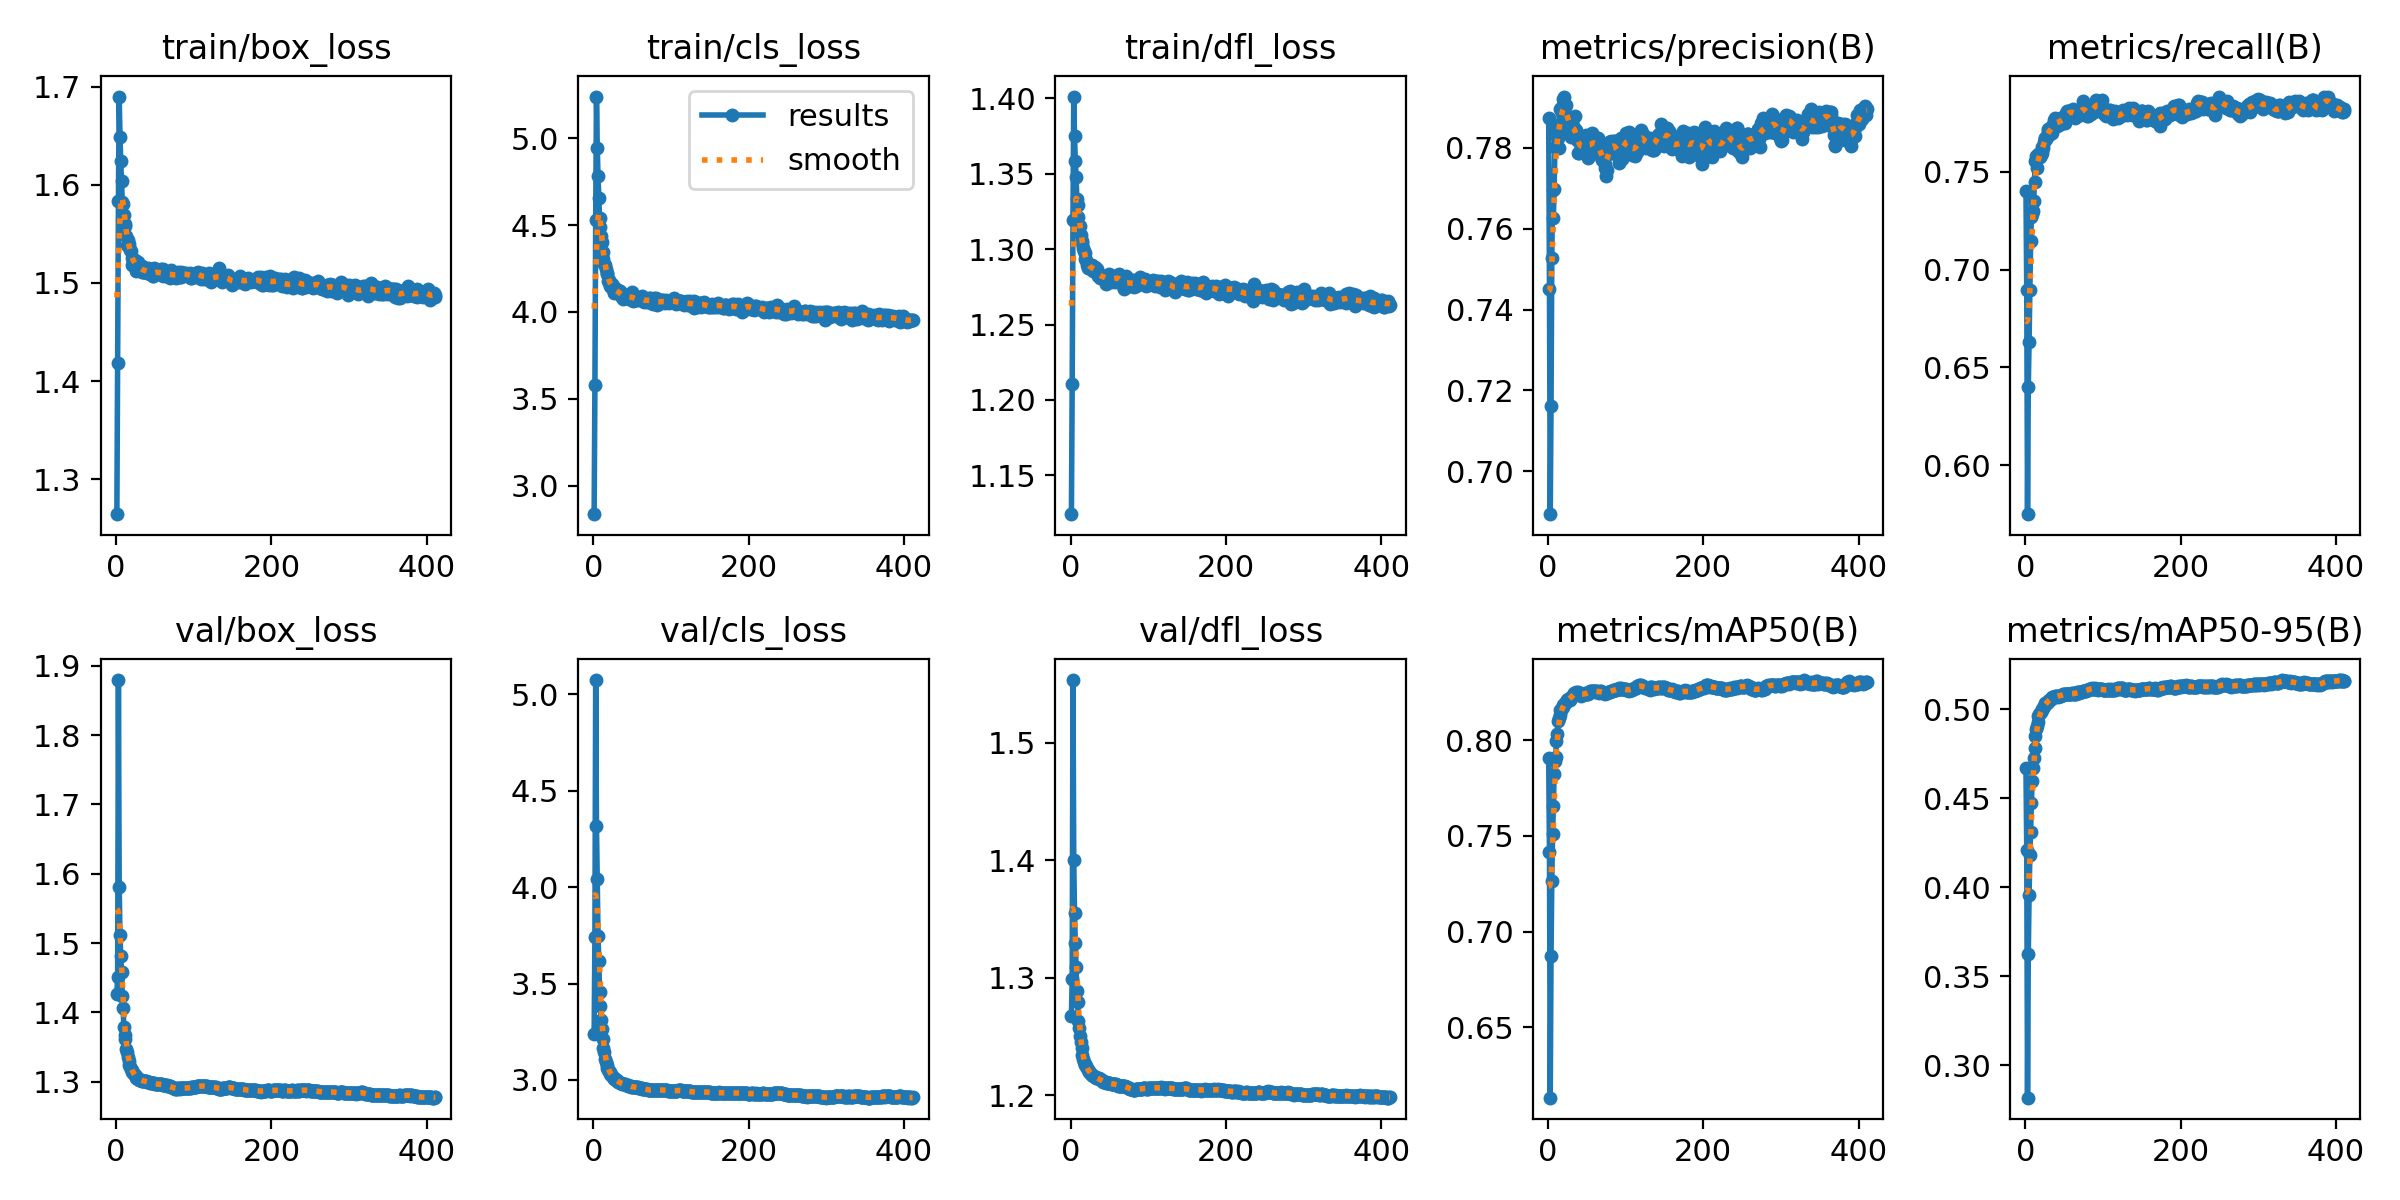
\includegraphics[width=\textwidth,height=0.58\textheight,keepaspectratio]{results_pgie.png}
  \end{center}

  \vspace{1mm}

  \begin{center}
    \scriptsize
    \textcolor{labelcolor}{Convergência estável após época 80 --- mAP estabiliza em $\sim$0,83.}
  \end{center}

  \vfill
\end{frame}

% --- Slide 27: PGIE - Avaliação ---
\begin{frame}{PGIE --- Avaliação}
  \smallskip
  \centering
  {\small Matriz de confusão normalizada e curvas Precision-Recall (5 classes, mAP@0,5 = 0,83).}

  \vspace{3mm}

  \begin{columns}[c]
    \begin{column}{0.48\textwidth}
      \centering
      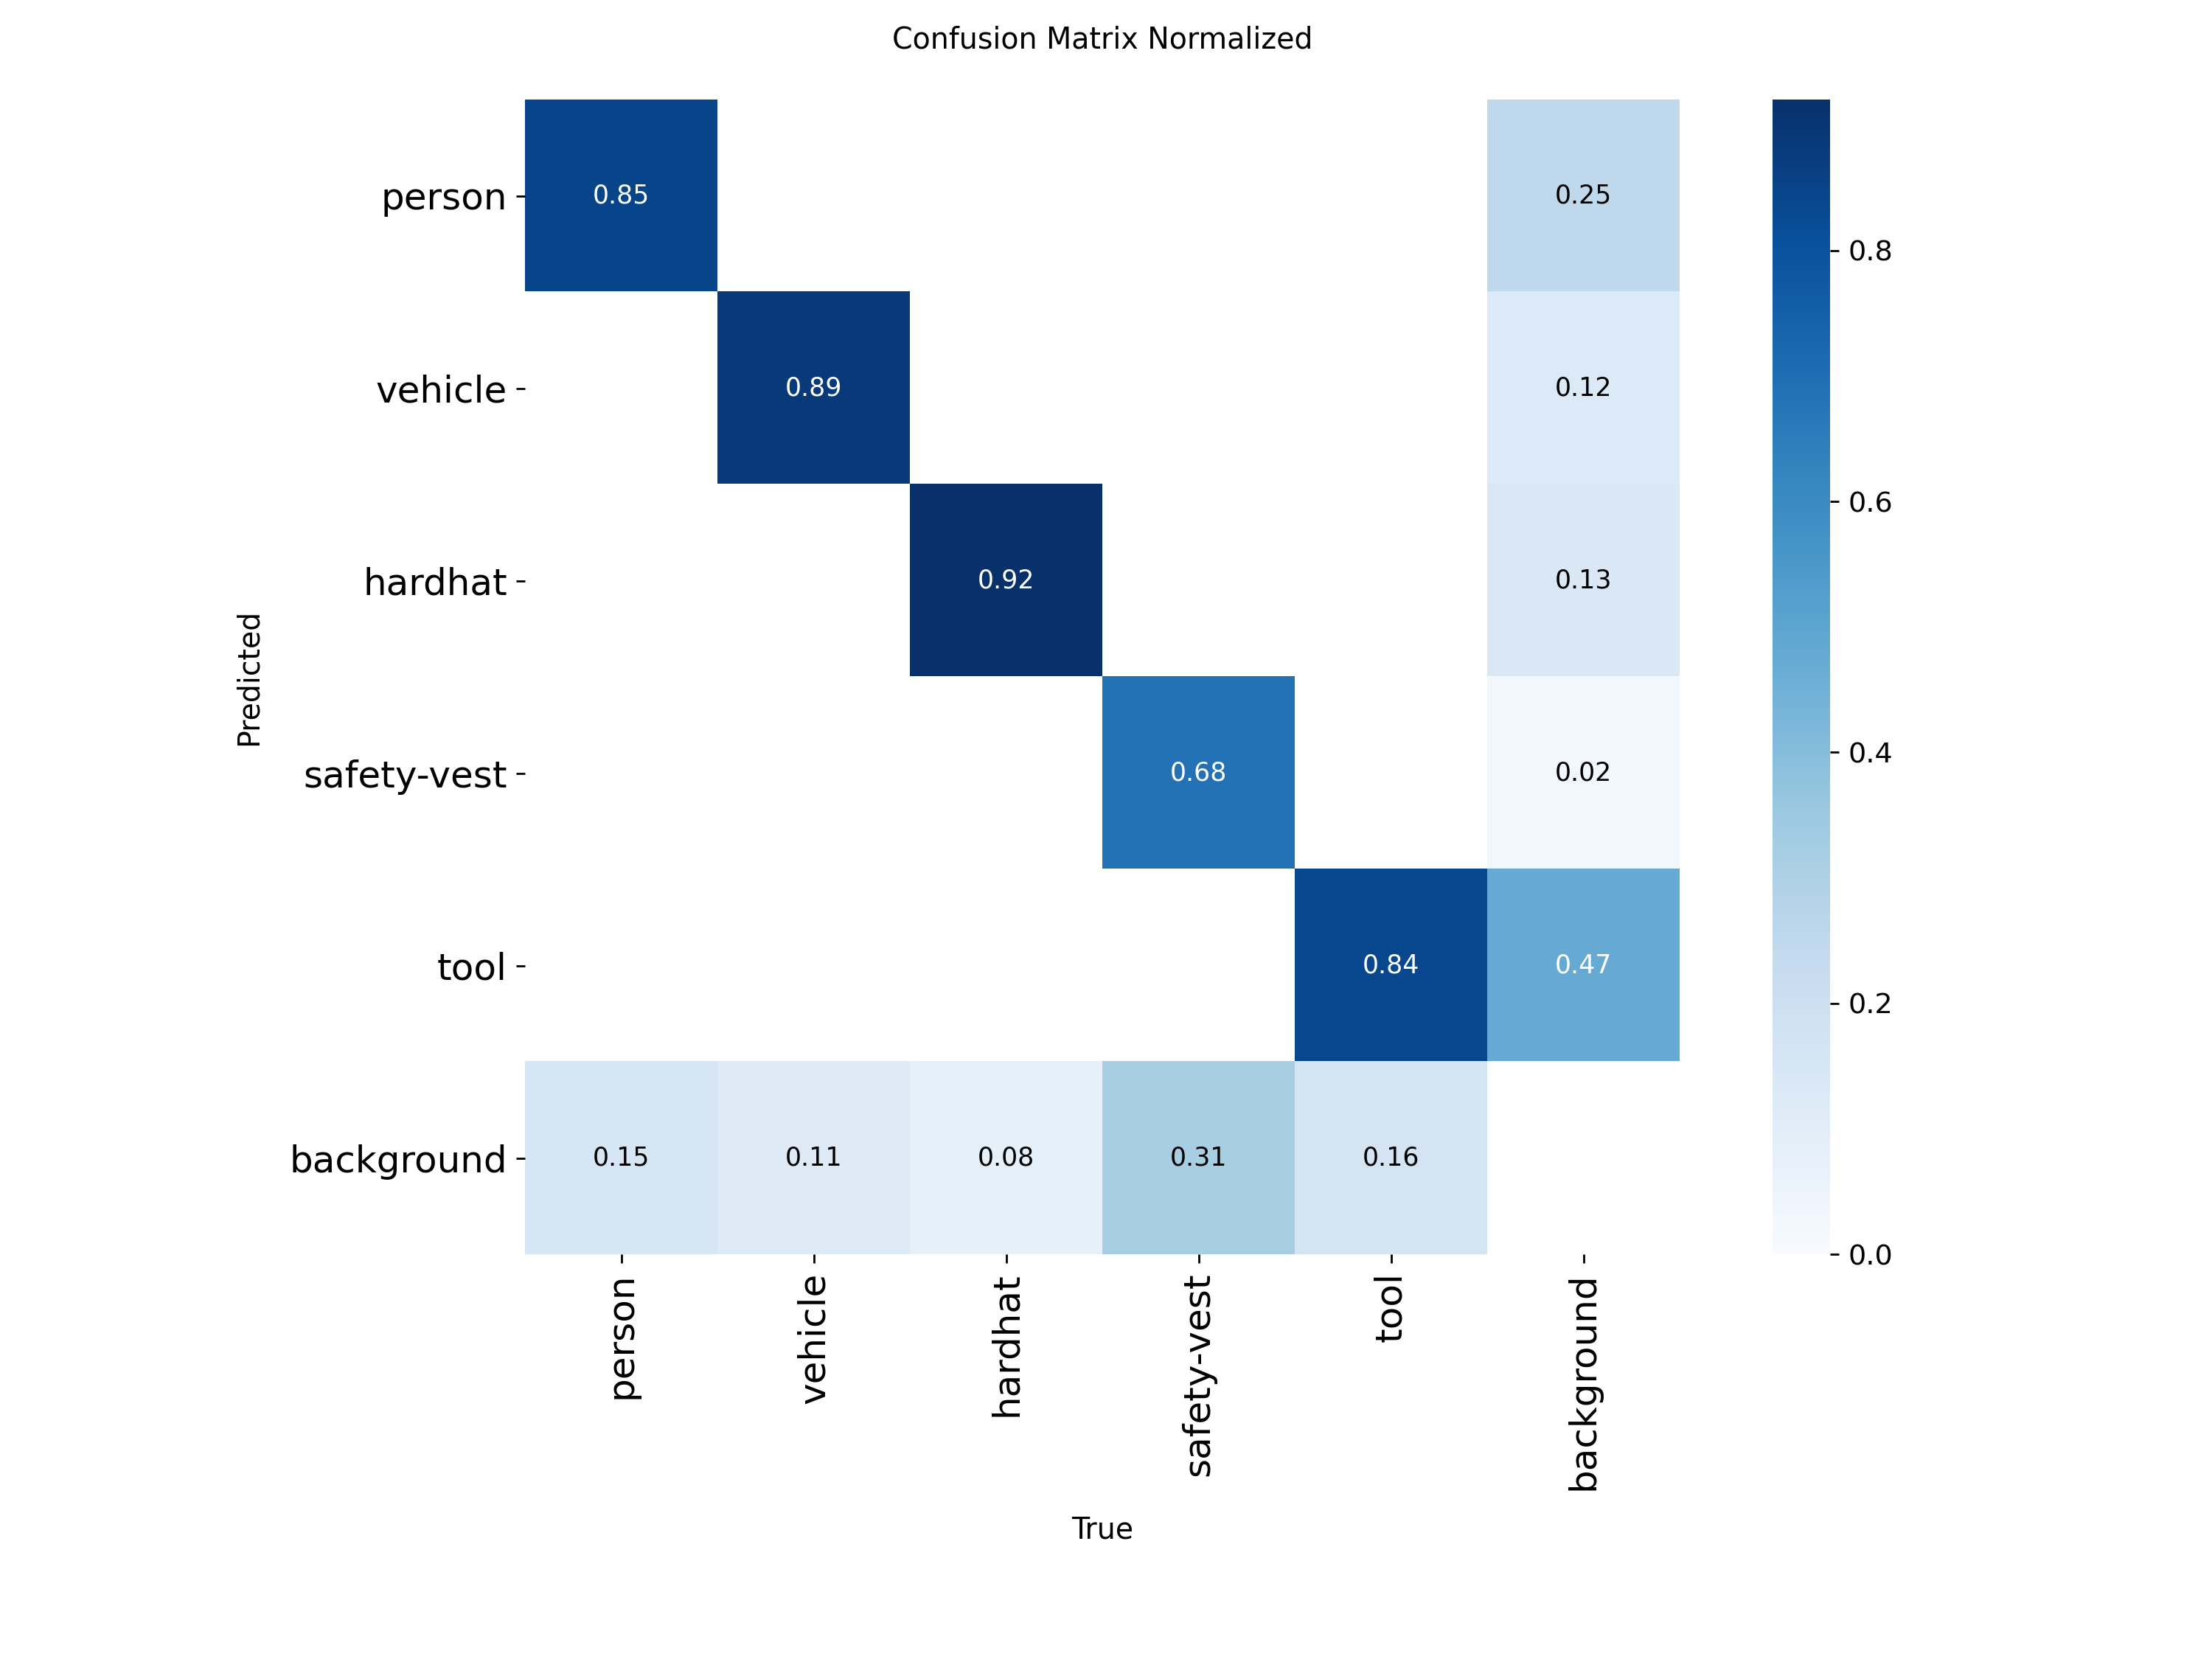
\includegraphics[width=\textwidth,height=0.60\textheight,keepaspectratio]{confusion_matrix_pgie.png}
    \end{column}
    \begin{column}{0.48\textwidth}
      \centering
      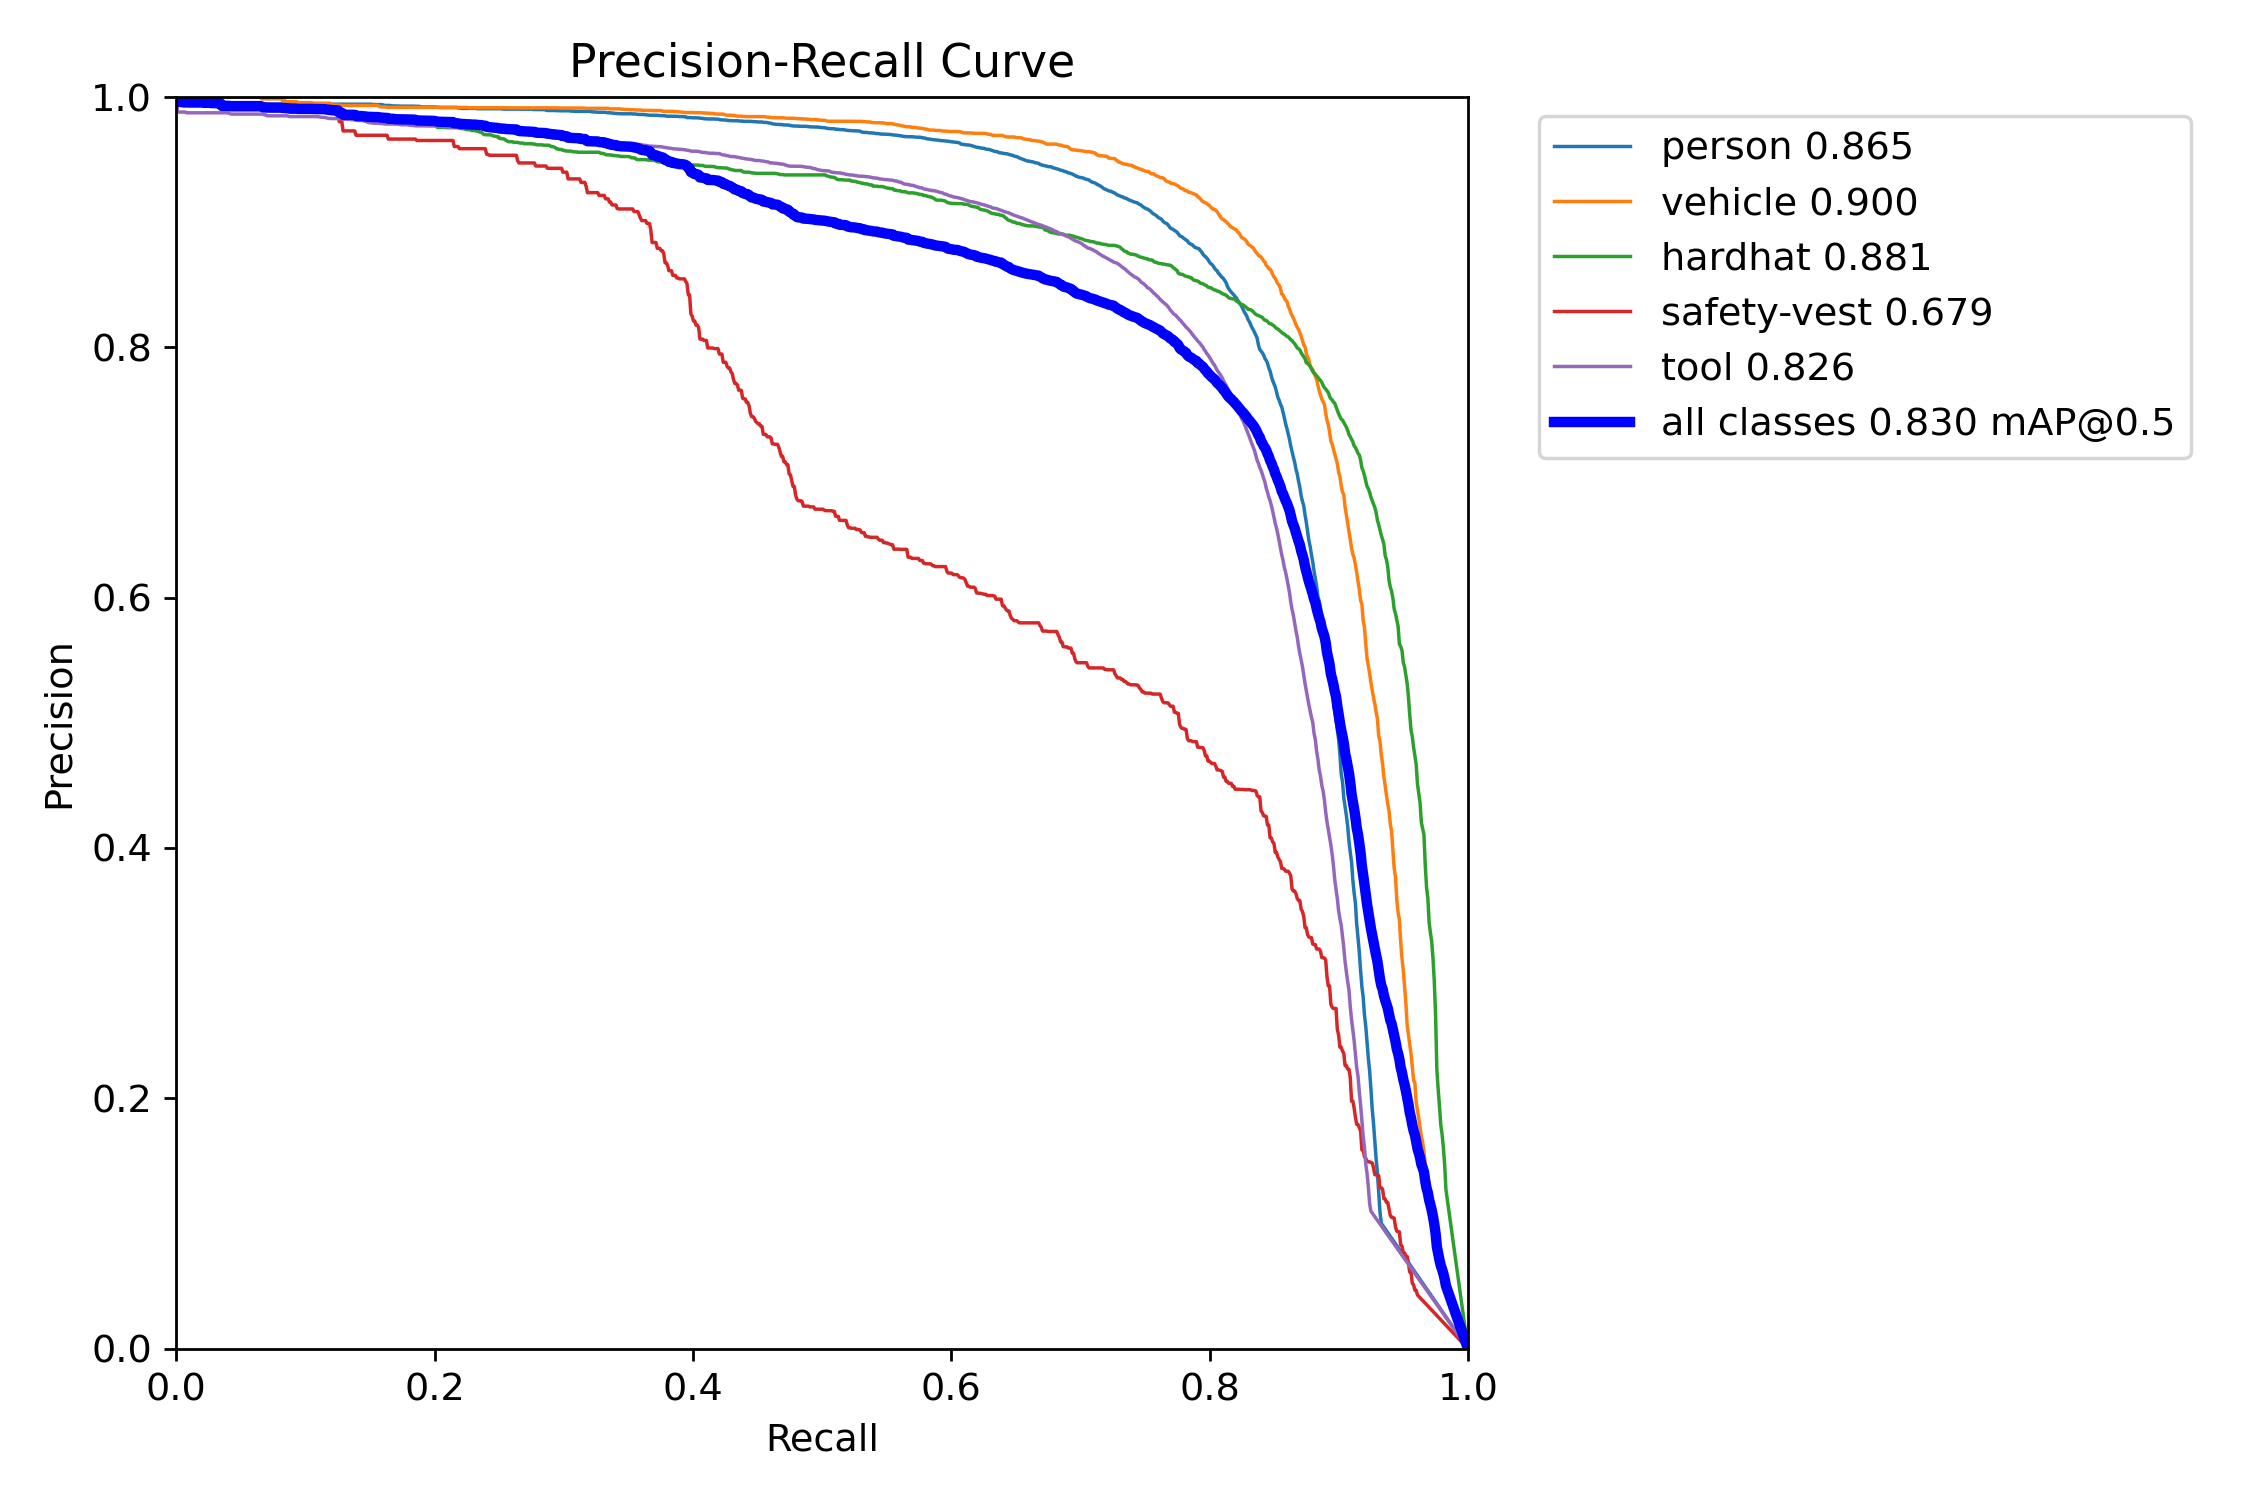
\includegraphics[width=\textwidth,height=0.60\textheight,keepaspectratio]{PR_curve_pgie.png}
    \end{column}
  \end{columns}

  \vspace{2mm}

  \begin{center}
    \footnotesize
    \textcolor{labelcolor}{%
      Todas com AP $\geq$ 0,68.
      Melhor: \textbf{Vehicle} (0,90).
      Pior: \textbf{Safety-vest} (0,68) --- poucas instâncias (6.500).}
  \end{center}

  \vfill
\end{frame}

% --- Slide 28: SGIE-EPI --- AP por Classe ---
\begin{frame}{SGIE-EPI --- AP por Classe}
  \vspace{-2mm}
  {\small\color{sublabelcolor}%
    Desempenho das 14 classes de EPI ordenadas por AP@0,5 --- mAP geral = 0,77.}

  \vspace{1mm}

  \begin{center}
    \resizebox{0.95\textwidth}{!}{% ============================================================================
% Gráfico de Barras Horizontais - AP@0.5 por Classe do SGIE-EPI
% Para dissertação de mestrado PPGC/UFRGS
% Uso: % ============================================================================
% Gráfico de Barras Horizontais - AP@0.5 por Classe do SGIE-EPI
% Para dissertação de mestrado PPGC/UFRGS
% Uso: \input{figuras/diagrama_sgie_epi_distribuicao.tex}
% ============================================================================

\begin{tikzpicture}
\begin{axis}[
    xbar,
    width=0.92\textwidth,
    height=10cm,
    bar width=8pt,
    enlarge y limits=0.05,
    xlabel={AP@0.5},
    xlabel style={font=\small},
    xmin=0,
    xmax=1.12,
    xtick={0, 0.2, 0.4, 0.6, 0.8, 1.0},
    xticklabel style={font=\footnotesize},
    ytick=data,
    yticklabels={
        NO-Safety Vest,
        Mask,
        Safety Cone,
        NO-Mask,
        Safety Vest,
        NO-Hardhat,
        Fall-Detected,
        Hardhat,
        NO-Gloves,
        Person,
        NO-Goggles,
        Ladder,
        Gloves,
        Goggles
    },
    yticklabel style={font=\footnotesize},
    y dir=normal,
    nodes near coords,
    nodes near coords align={horizontal},
    nodes near coords style={font=\scriptsize, /pgf/number format/fixed, /pgf/number format/precision=3},
    every node near coord/.append style={anchor=west, xshift=1pt},
    grid=major,
    grid style={gray!20, very thin},
    major x grid style={gray!30, thin},
    tick align=outside,
    axis line style={gray!60},
    legend style={at={(0.97,0.03)}, anchor=south east, font=\footnotesize},
]

% Barras com cores baseadas no desempenho
% AP >= 0.90: detectioncolor (verde escuro) - excelente
% AP >= 0.70: headcolor (verde) - bom
% AP >= 0.50: neckcolor (roxo) - moderado
% AP < 0.50: skipcolor (vermelho) - baixo

% Faixa excelente (AP >= 0.90)
\addplot[
    xbar,
    fill=detectioncolor!70,
    draw=detectioncolor!90,
    bar width=8pt,
] coordinates {
    (0.971, 13)
    (0.948, 12)
    (0.946, 11)
    (0.939, 10)
    (0.931, 9)
    (0.908, 8)
};

% Faixa boa (0.70 <= AP < 0.90)
\addplot[
    xbar,
    fill=headcolor!50,
    draw=headcolor!80,
    bar width=8pt,
] coordinates {
    (0.896, 7)
    (0.859, 6)
    (0.724, 5)
    (0.682, 4)
};

% Faixa moderada (0.50 <= AP < 0.70)
\addplot[
    xbar,
    fill=neckcolor!40,
    draw=neckcolor!70,
    bar width=8pt,
] coordinates {
    (0.611, 3)
    (0.608, 2)
    (0.524, 1)
};

% Faixa baixa (AP < 0.50)
\addplot[
    xbar,
    fill=skipcolor!40,
    draw=skipcolor!70,
    bar width=8pt,
] coordinates {
    (0.236, 0)
};

\legend{AP $\geq$ 0{,}90, 0{,}70 $\leq$ AP $<$ 0{,}90, 0{,}50 $\leq$ AP $<$ 0{,}70, AP $<$ 0{,}50}

\end{axis}
\end{tikzpicture}

% ============================================================================

\begin{tikzpicture}
\begin{axis}[
    xbar,
    width=0.92\textwidth,
    height=10cm,
    bar width=8pt,
    enlarge y limits=0.05,
    xlabel={AP@0.5},
    xlabel style={font=\small},
    xmin=0,
    xmax=1.12,
    xtick={0, 0.2, 0.4, 0.6, 0.8, 1.0},
    xticklabel style={font=\footnotesize},
    ytick=data,
    yticklabels={
        NO-Safety Vest,
        Mask,
        Safety Cone,
        NO-Mask,
        Safety Vest,
        NO-Hardhat,
        Fall-Detected,
        Hardhat,
        NO-Gloves,
        Person,
        NO-Goggles,
        Ladder,
        Gloves,
        Goggles
    },
    yticklabel style={font=\footnotesize},
    y dir=normal,
    nodes near coords,
    nodes near coords align={horizontal},
    nodes near coords style={font=\scriptsize, /pgf/number format/fixed, /pgf/number format/precision=3},
    every node near coord/.append style={anchor=west, xshift=1pt},
    grid=major,
    grid style={gray!20, very thin},
    major x grid style={gray!30, thin},
    tick align=outside,
    axis line style={gray!60},
    legend style={at={(0.97,0.03)}, anchor=south east, font=\footnotesize},
]

% Barras com cores baseadas no desempenho
% AP >= 0.90: detectioncolor (verde escuro) - excelente
% AP >= 0.70: headcolor (verde) - bom
% AP >= 0.50: neckcolor (roxo) - moderado
% AP < 0.50: skipcolor (vermelho) - baixo

% Faixa excelente (AP >= 0.90)
\addplot[
    xbar,
    fill=detectioncolor!70,
    draw=detectioncolor!90,
    bar width=8pt,
] coordinates {
    (0.971, 13)
    (0.948, 12)
    (0.946, 11)
    (0.939, 10)
    (0.931, 9)
    (0.908, 8)
};

% Faixa boa (0.70 <= AP < 0.90)
\addplot[
    xbar,
    fill=headcolor!50,
    draw=headcolor!80,
    bar width=8pt,
] coordinates {
    (0.896, 7)
    (0.859, 6)
    (0.724, 5)
    (0.682, 4)
};

% Faixa moderada (0.50 <= AP < 0.70)
\addplot[
    xbar,
    fill=neckcolor!40,
    draw=neckcolor!70,
    bar width=8pt,
] coordinates {
    (0.611, 3)
    (0.608, 2)
    (0.524, 1)
};

% Faixa baixa (AP < 0.50)
\addplot[
    xbar,
    fill=skipcolor!40,
    draw=skipcolor!70,
    bar width=8pt,
] coordinates {
    (0.236, 0)
};

\legend{AP $\geq$ 0{,}90, 0{,}70 $\leq$ AP $<$ 0{,}90, 0{,}50 $\leq$ AP $<$ 0{,}70, AP $<$ 0{,}50}

\end{axis}
\end{tikzpicture}
}
  \end{center}

  \vspace{1mm}

  \begin{center}
    \scriptsize
    \textcolor{detectioncolor!80!black}{$\blacksquare$} 6 classes com AP $>$ 0,90 (Goggles, Gloves, Ladder, NO-Goggles, Person, NO-Gloves).\quad
    \textcolor{skipcolor!80!black}{$\blacksquare$} NO-Safety Vest (0,24) --- poucas amostras (890).
  \end{center}

  \vfill
\end{frame}

% --- Slide 29: SGIE-EPI --- Avaliação ---
\begin{frame}{SGIE-EPI --- Avaliação}
  \smallskip
  \centering
  {\small Matriz de confusão e curvas PR para 14 classes de EPIs e situações de risco.}

  \vspace{3mm}

  \begin{columns}[c]
    \begin{column}{0.48\textwidth}
      \centering
      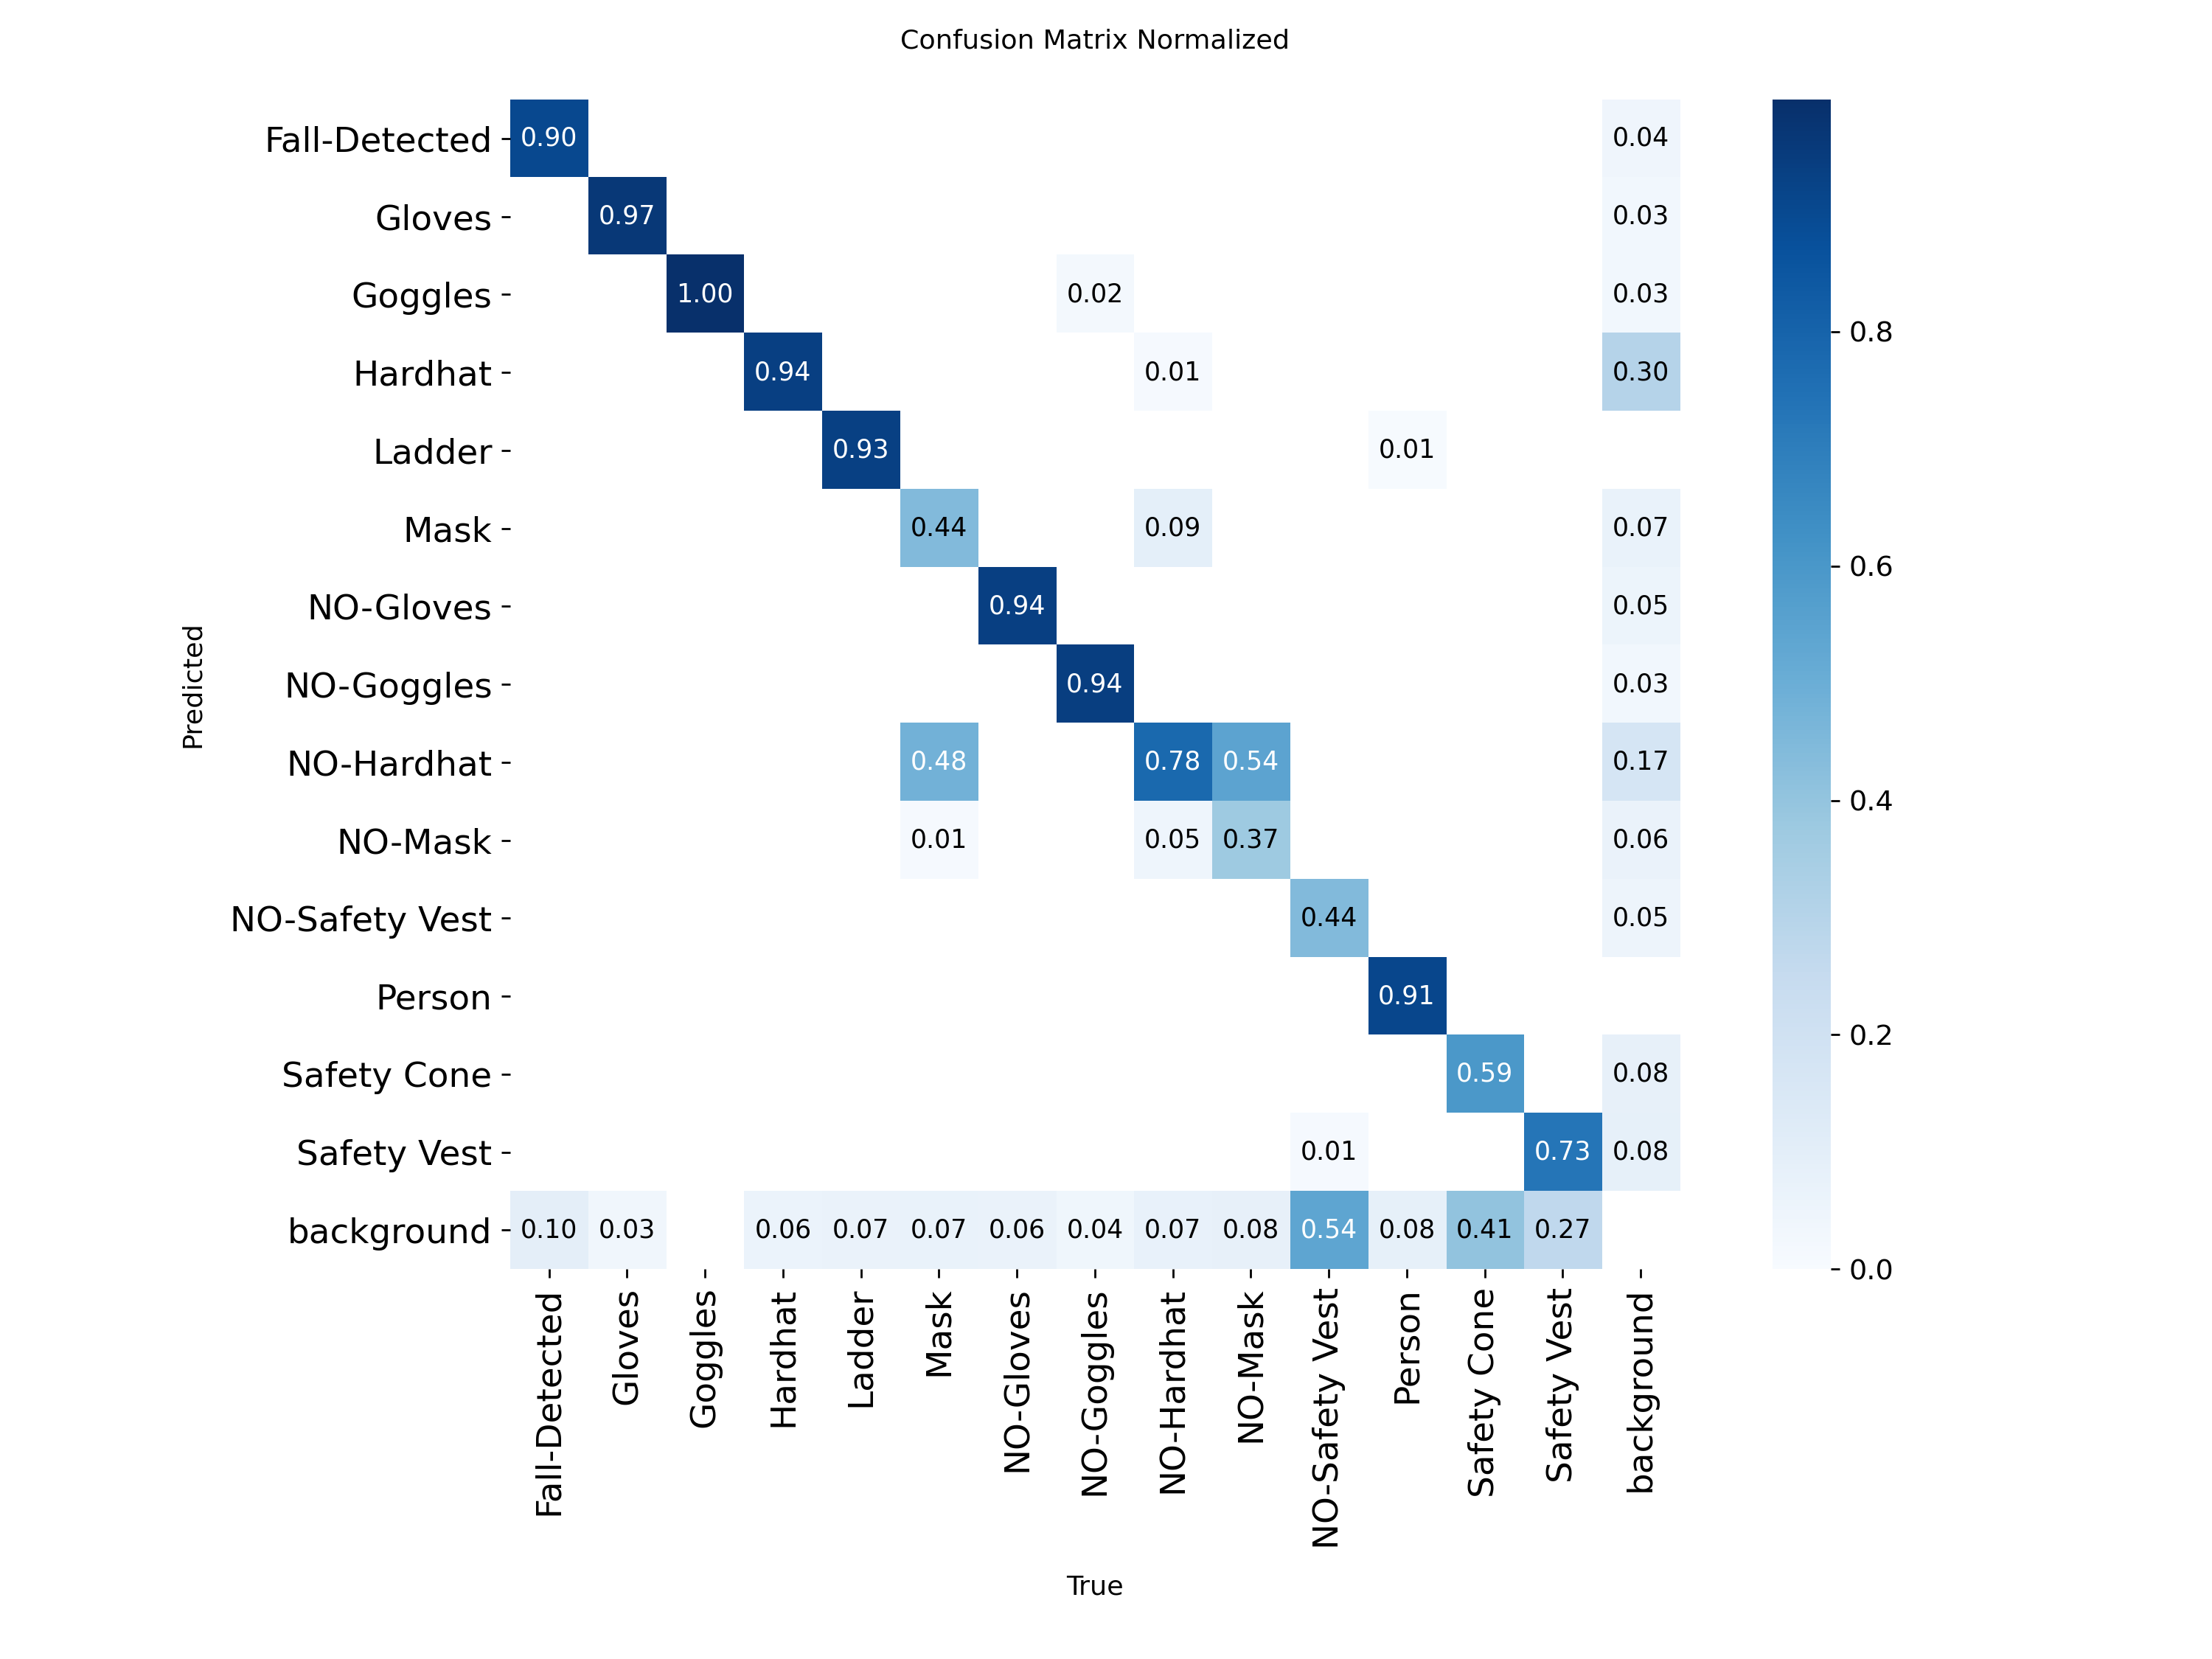
\includegraphics[width=\textwidth,height=0.65\textheight,keepaspectratio]{confusion_matrix_sgie_epi.png}
    \end{column}
    \begin{column}{0.48\textwidth}
      \centering
      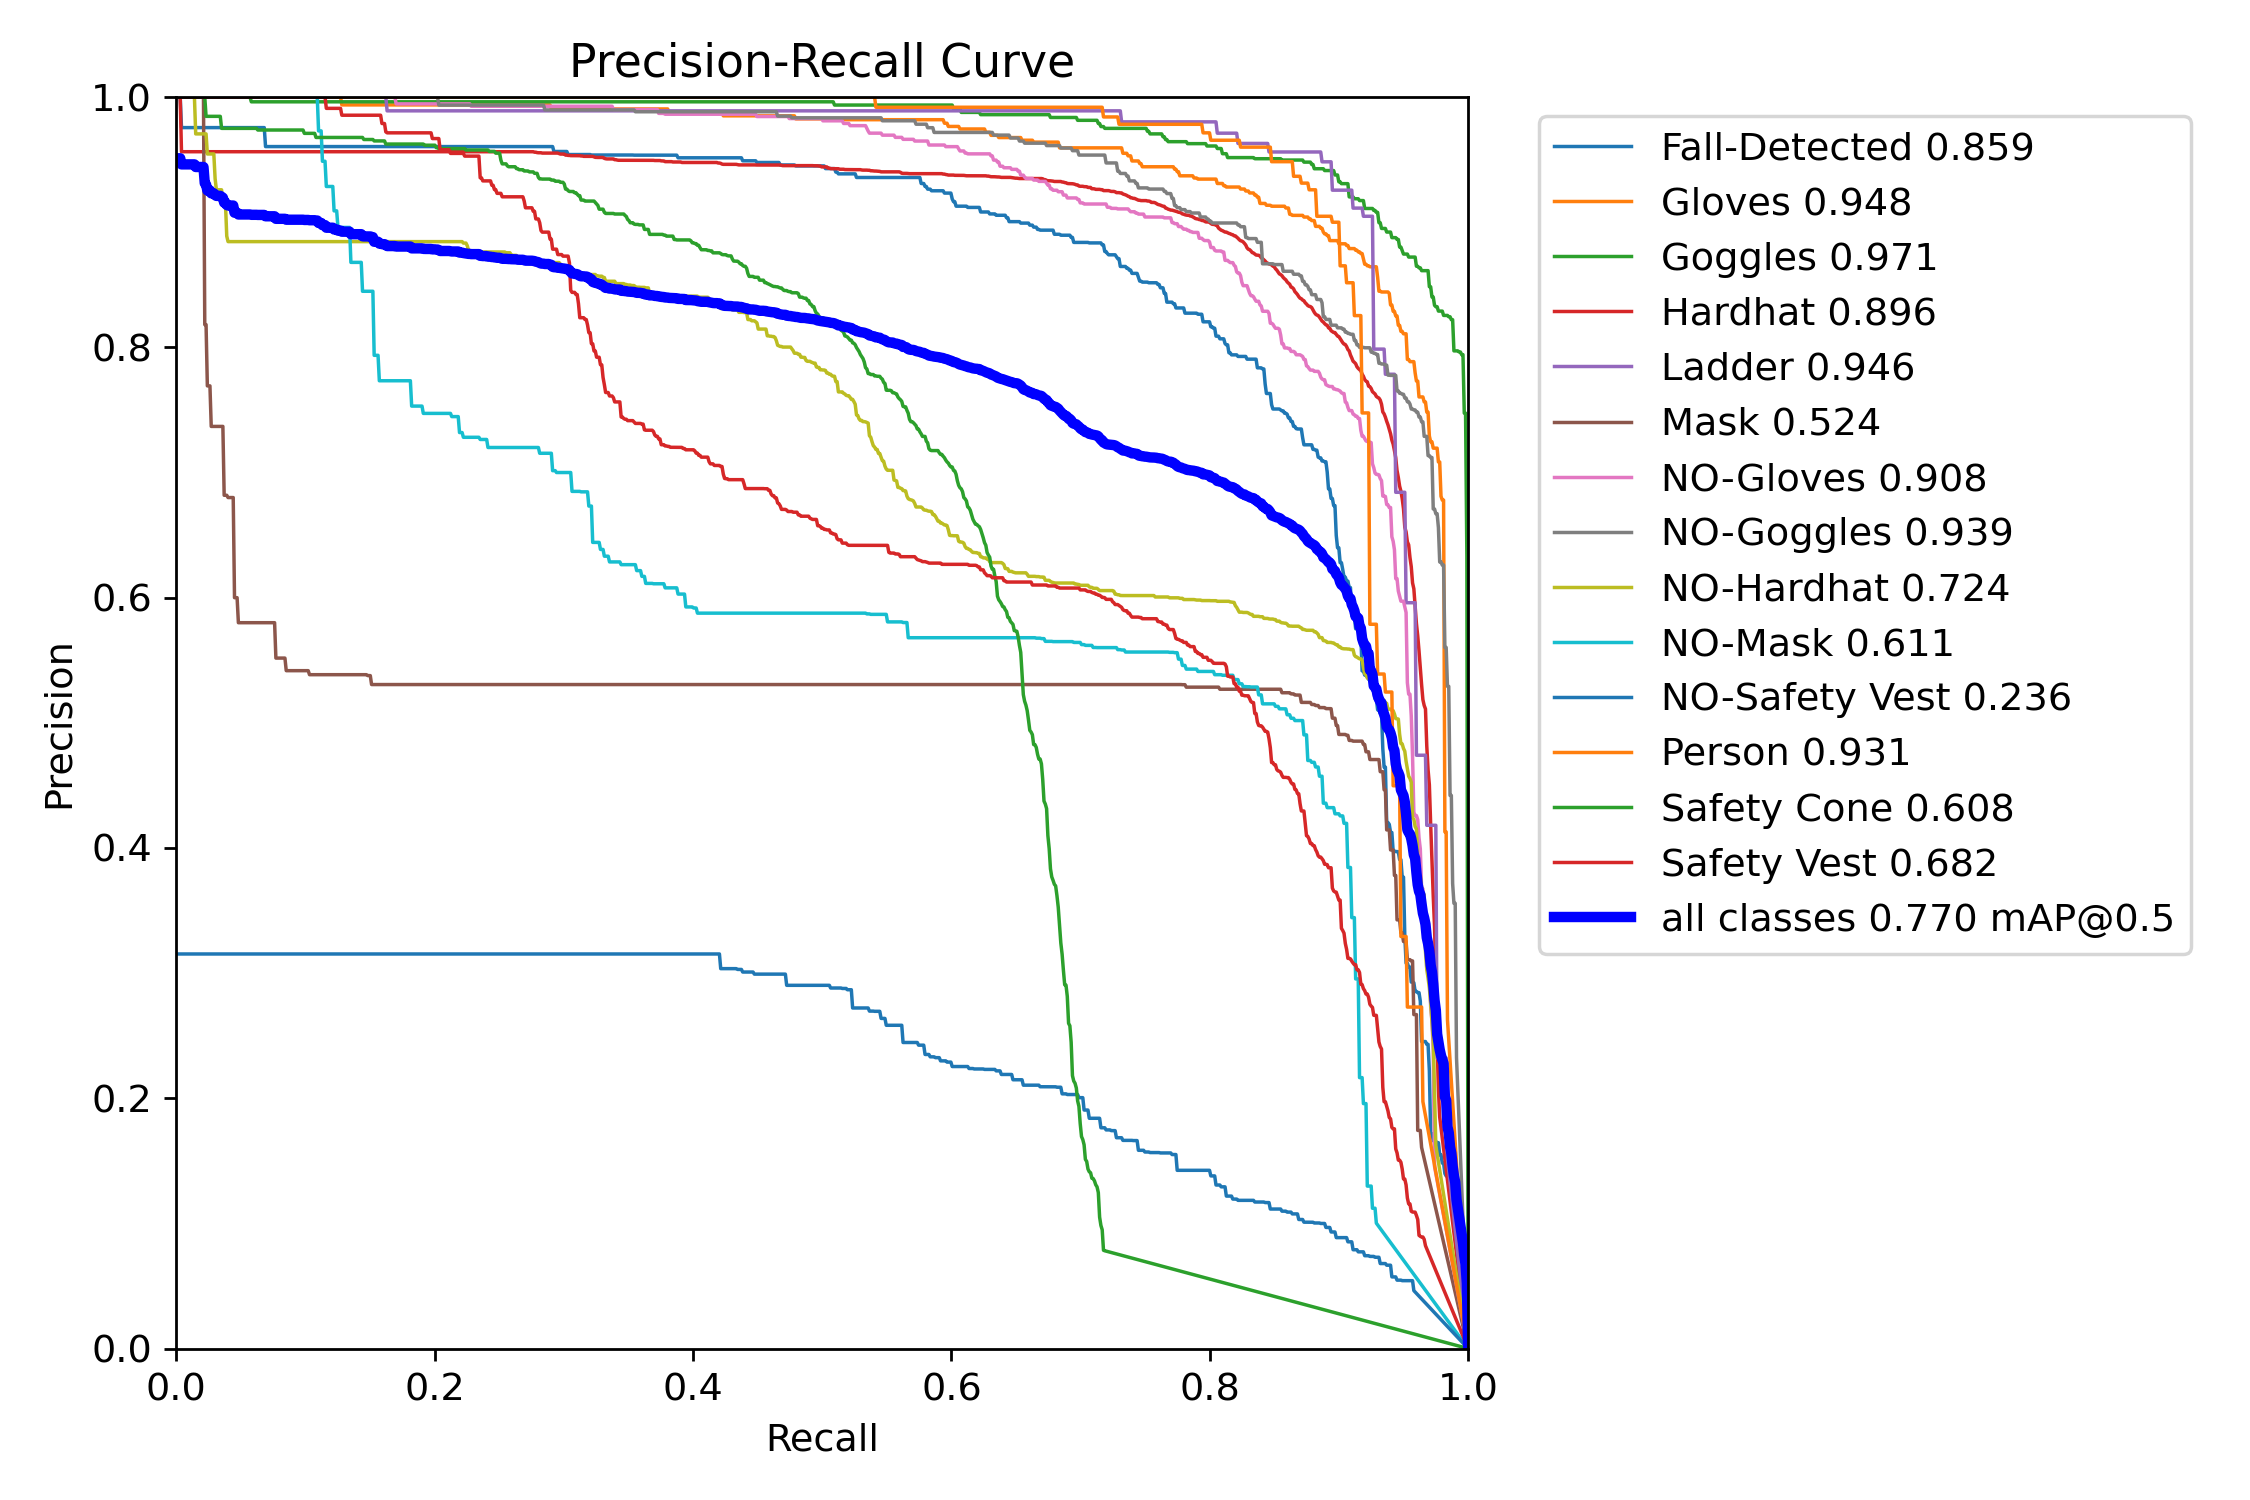
\includegraphics[width=\textwidth,height=0.65\textheight,keepaspectratio]{PR_curve_sgie_epi.png}
    \end{column}
  \end{columns}

  \vspace{3mm}

  \begin{center}
    \footnotesize
    \textcolor{labelcolor}{%
      mAP@0,5 = 0,77 com 14 classes. Confusões principais: Safety Vest $\leftrightarrow$ NO-Safety Vest\\
      e Mask $\leftrightarrow$ NO-Mask --- classes de ausência são inerentemente ambíguas.}
  \end{center}

  \vfill
\end{frame}

% --- Slide 30: SGIE-Maquinário --- Avaliação ---
\begin{frame}{SGIE-Maquinário --- Avaliação}
  \smallskip
  \centering
  {\small Melhor SGIE: mAP@0,5 = 0,84 com 9 classes de maquinário pesado.}

  \vspace{3mm}

  \begin{columns}[c]
    \begin{column}{0.48\textwidth}
      \centering
      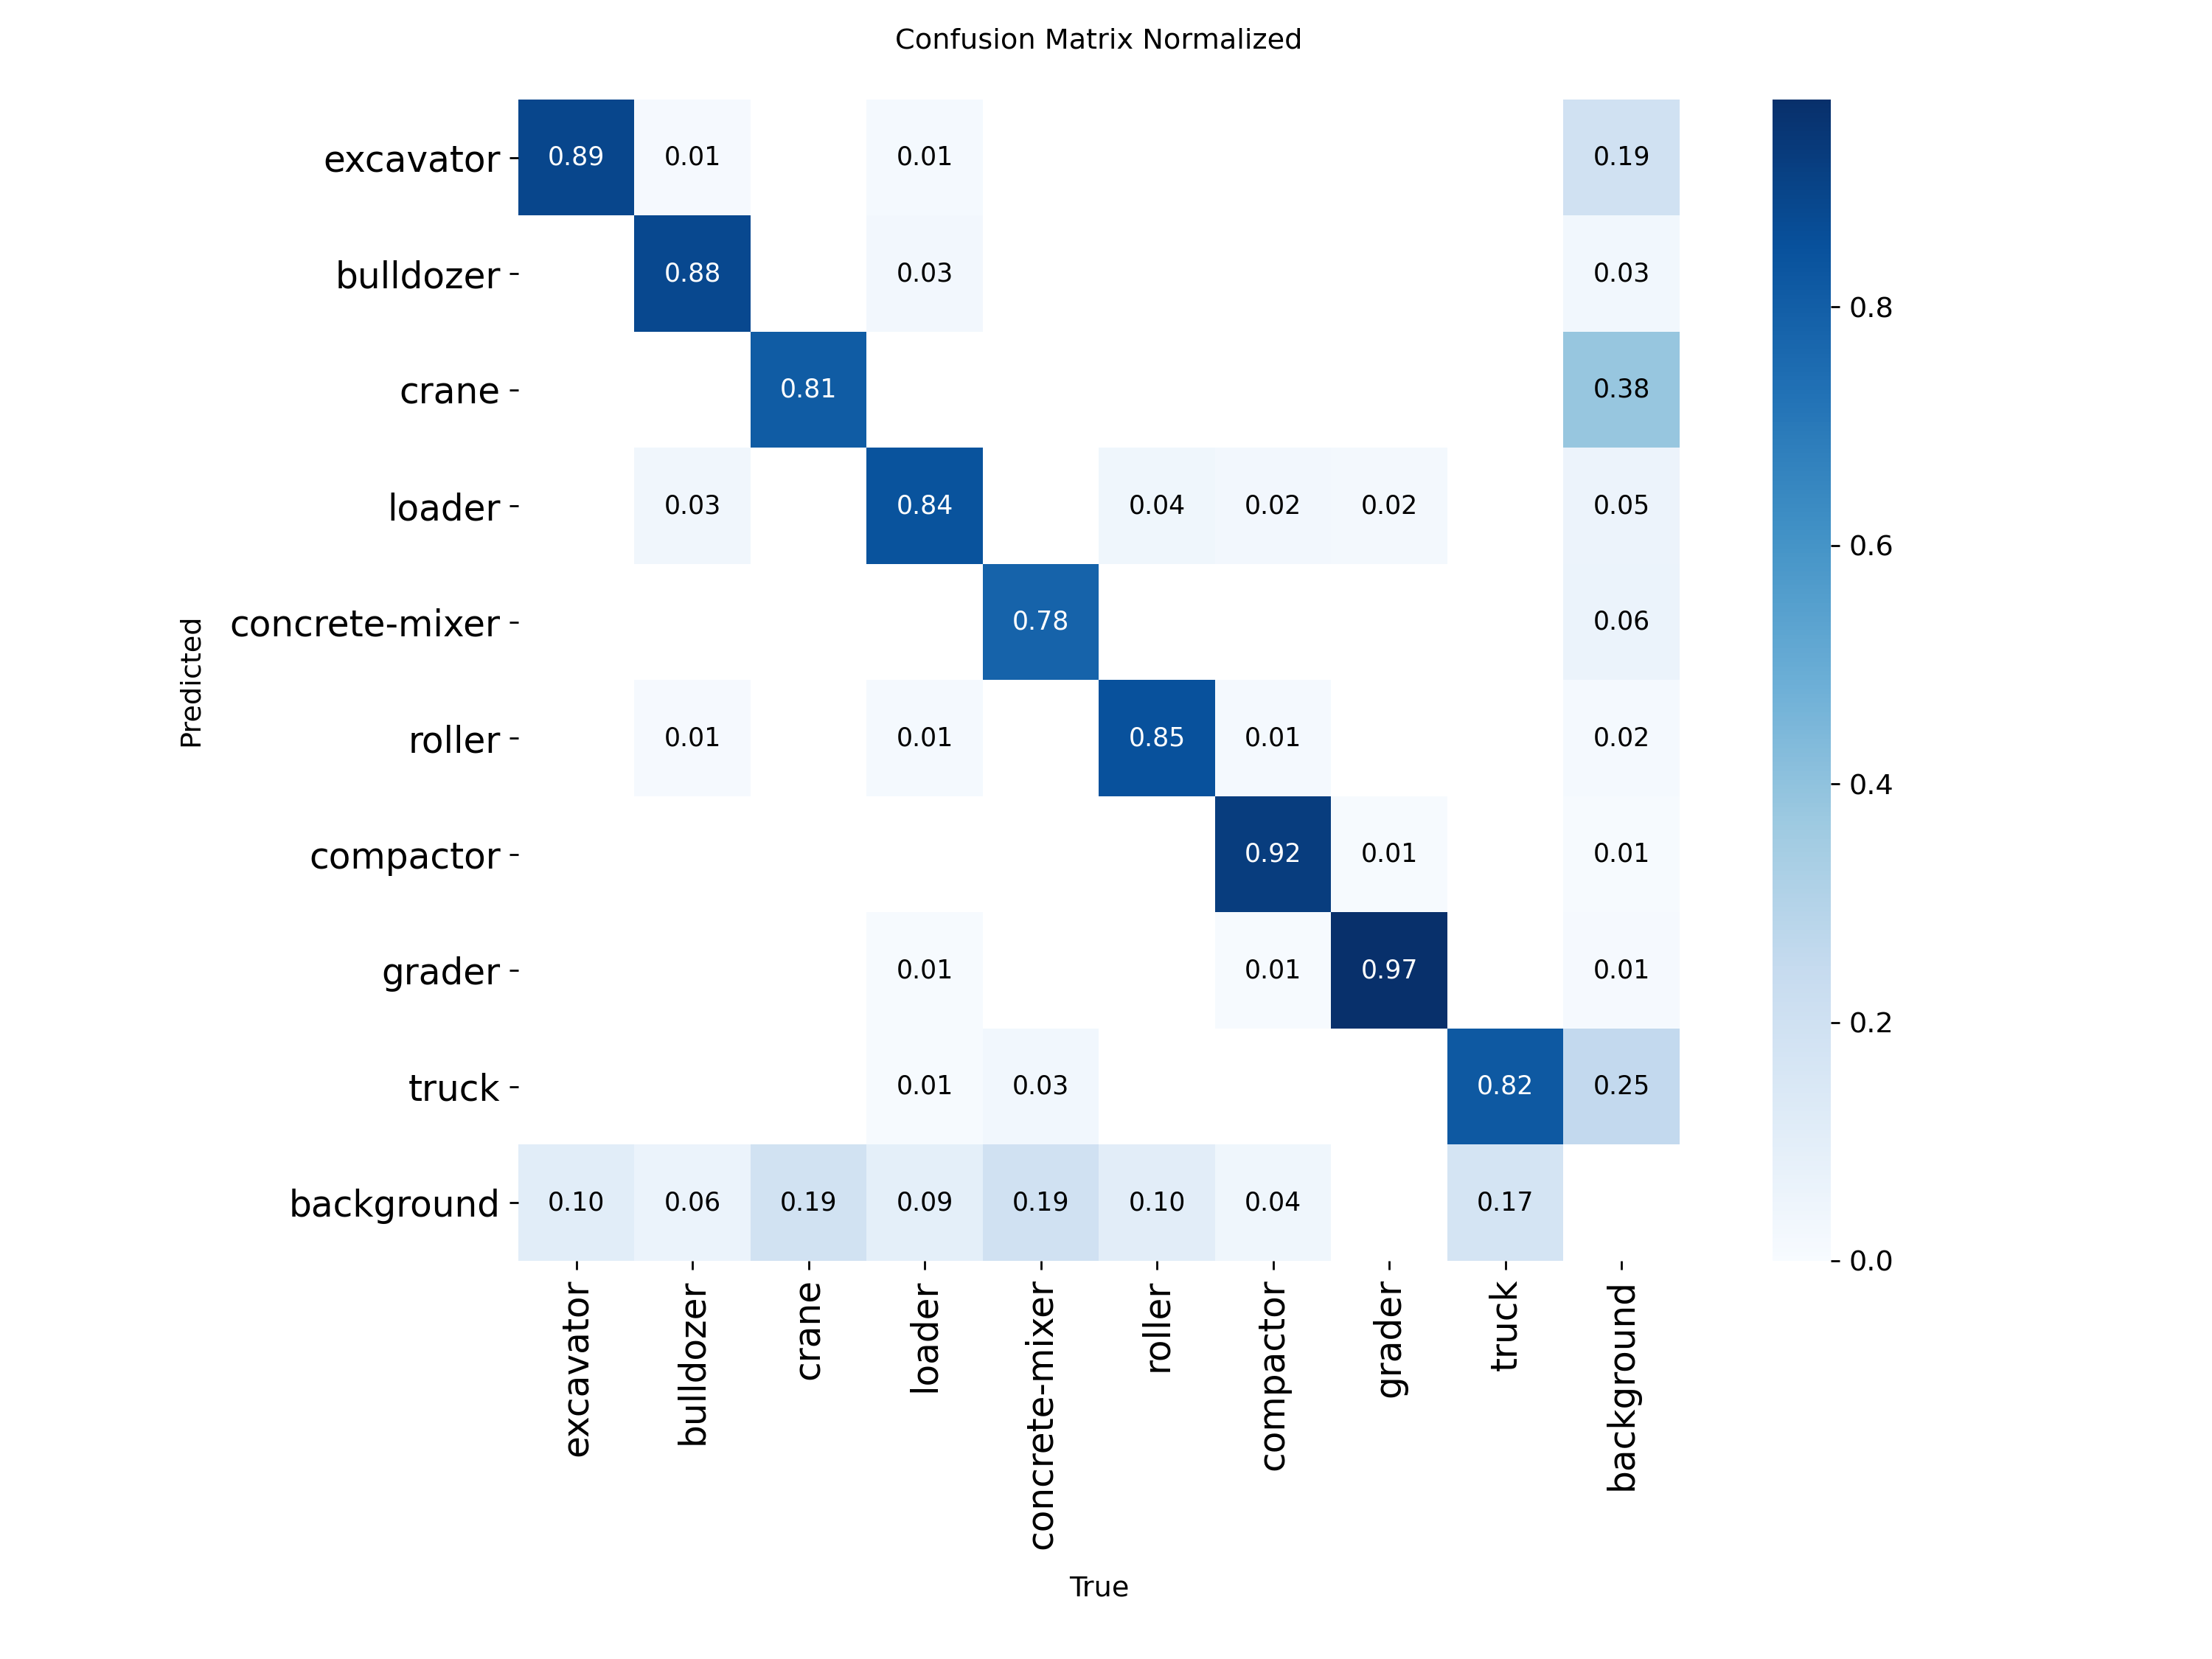
\includegraphics[width=\textwidth,height=0.60\textheight,keepaspectratio]{confusion_matrix_sgie_machinery.png}
    \end{column}
    \begin{column}{0.48\textwidth}
      \centering
      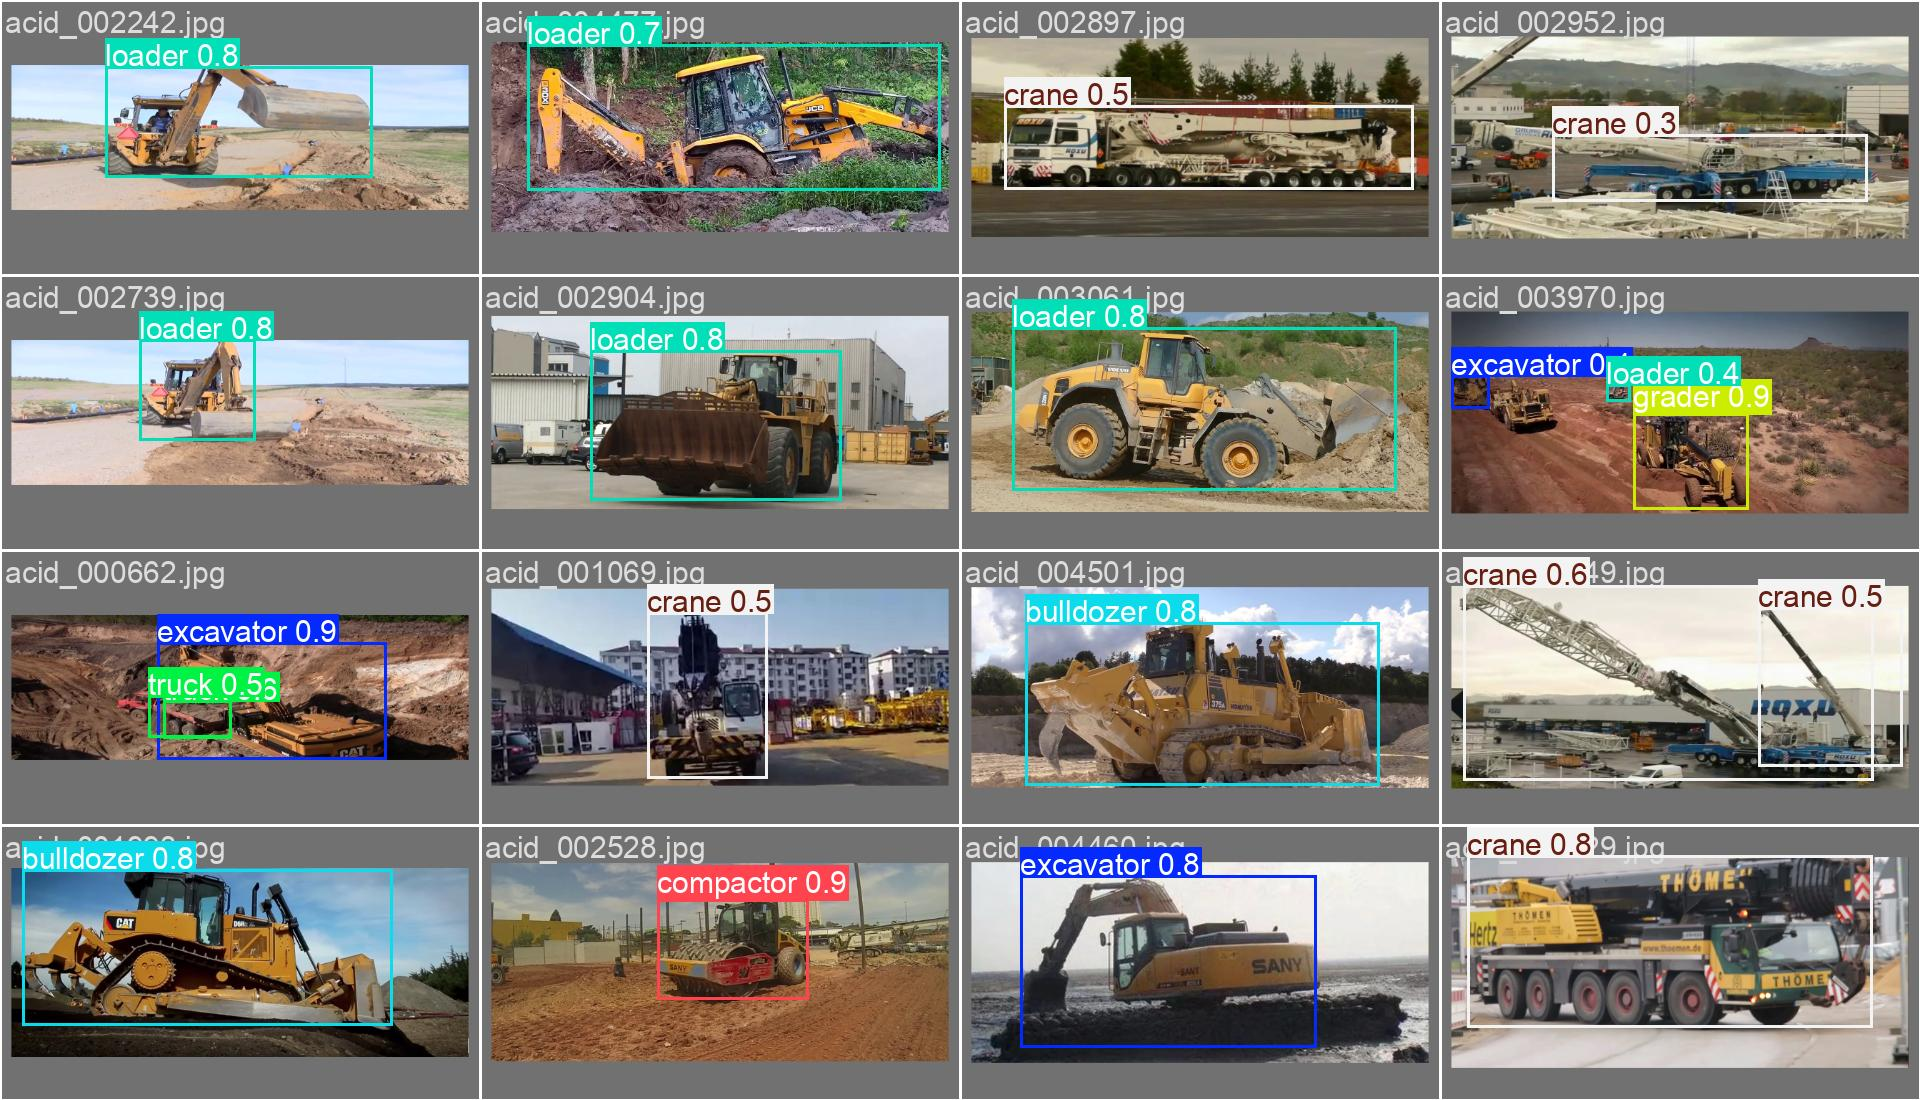
\includegraphics[width=\textwidth,height=0.68\textheight,keepaspectratio]{val_pred_sgie_machinery.jpg}
    \end{column}
  \end{columns}

  \vspace{3mm}

  \begin{center}
    \footnotesize
    \textcolor{labelcolor}{%
      Objetos grandes e visualmente distintos favorecem alta precisão.
      Melhor: \textbf{Excavator} (0,91).
      Menor: \textbf{Grader} (0,77) --- menos amostras (350).}
  \end{center}

  \vfill
\end{frame}

% --- Slide 31: SGIE-Ferramentas ---
\begin{frame}{SGIE-Ferramentas --- Avalia\c{c}\~{a}o (\textbf{23 classes})}
  \vspace{-2mm}
  \begin{columns}[c]
    \begin{column}{0.48\textwidth}
      \centering
      {\small\textbf{Matriz de Confus\~{a}o}}\\[3pt]
      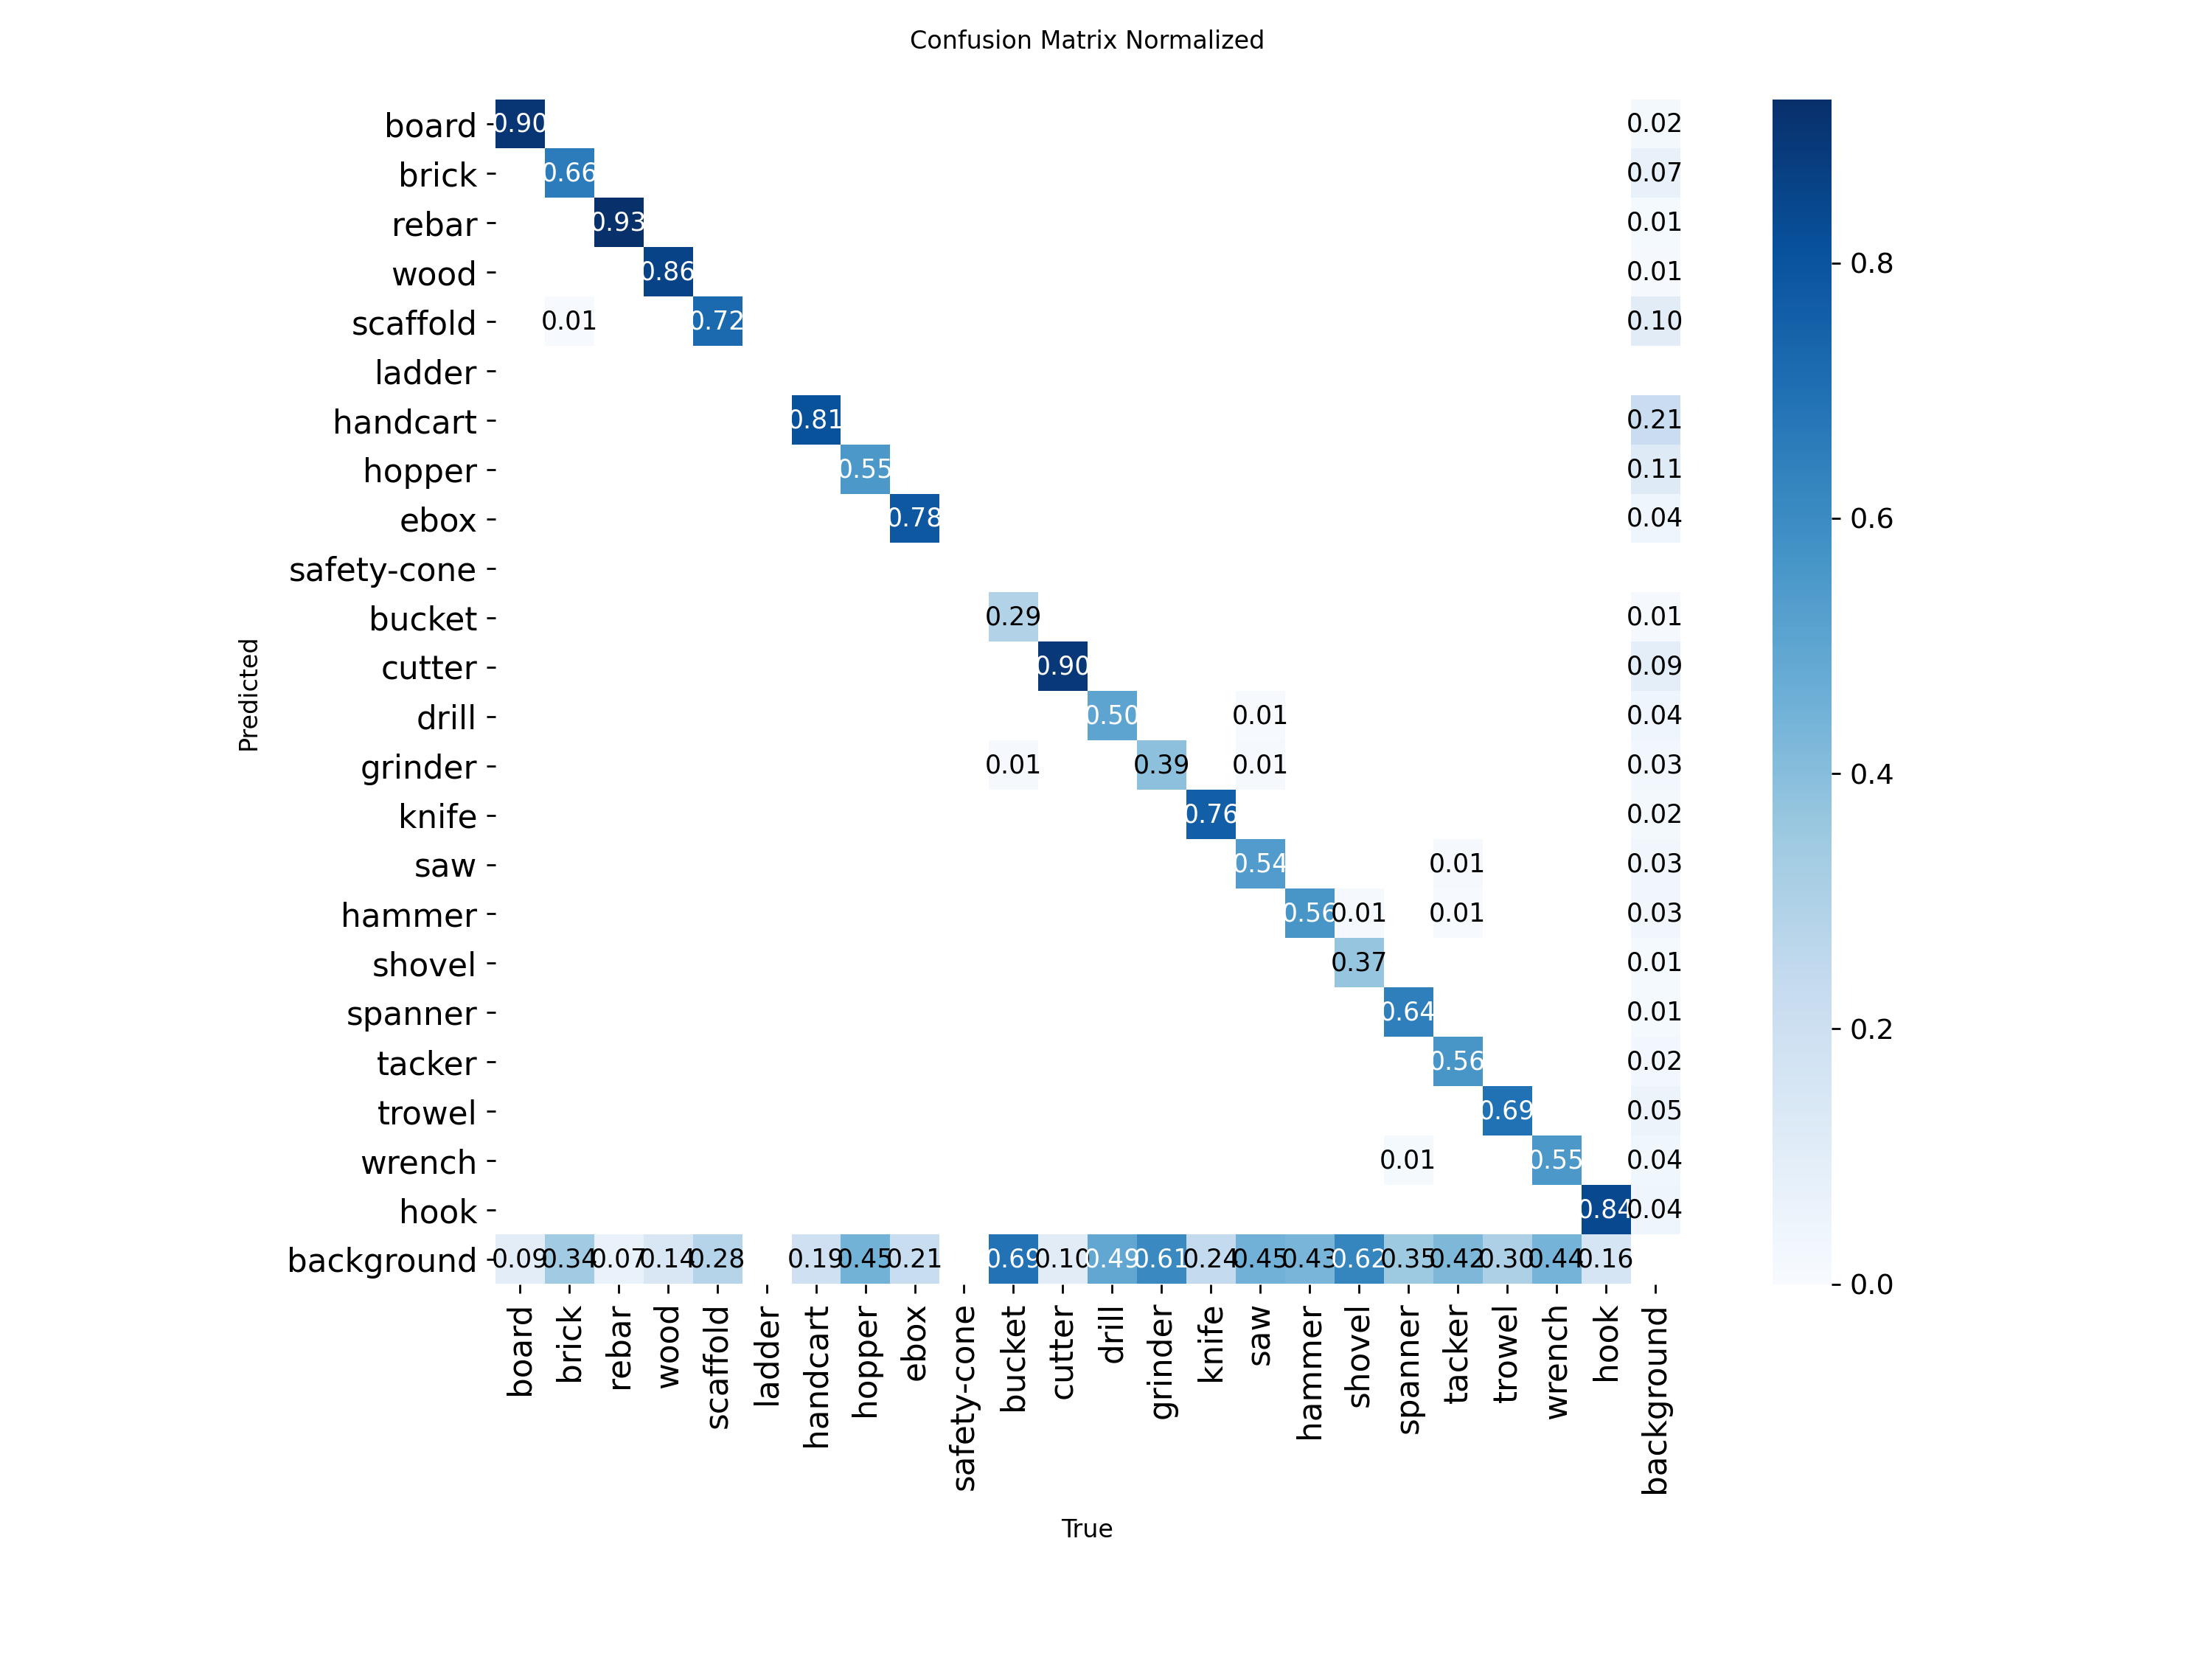
\includegraphics[width=\textwidth]{confusion_matrix_sgie_equipment.png}
    \end{column}
    \begin{column}{0.48\textwidth}
      \centering
      {\small\textbf{Predi\c{c}\~{o}es na Valida\c{c}\~{a}o}}\\[3pt]
      \adjustbox{clip, trim=0 0 {.5\width} 0}{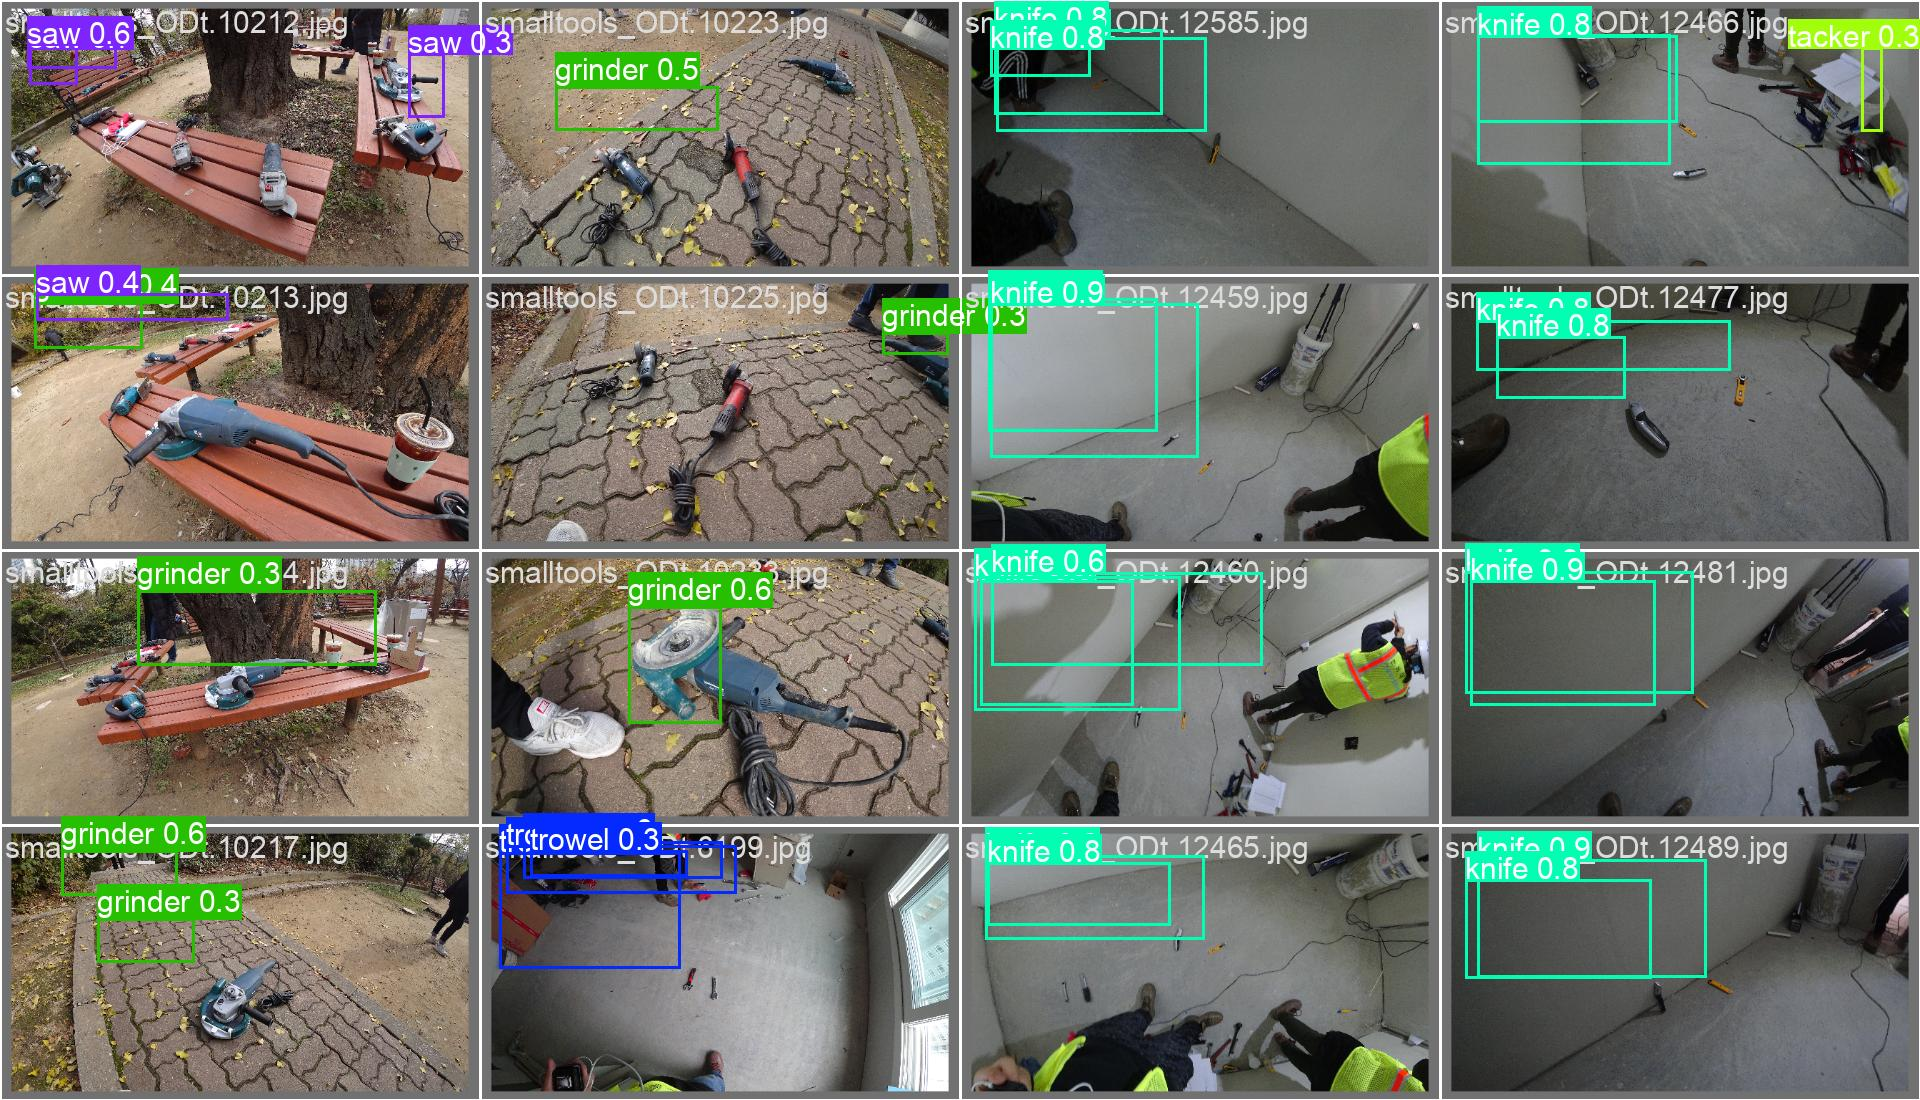
\includegraphics[width=\textwidth]{val_pred_sgie_equipment.jpg}}
    \end{column}
  \end{columns}

  \vspace{2mm}

  \begin{beamercolorbox}[wd=\textwidth, rounded=true, shadow=false]{block body}
    \centering
    {\scriptsize Maior desafio: \textbf{23 classes} com alta variabilidade.
    Objetos grandes (Cone: 0,86 / Ladder: 0,82) \textcolor{headcolor}{\textbf{superam 0,80}}.
    Ferramentas pequenas (Cutter: 0,54 / Trowel: 0,56) \textcolor{skipcolor}{\textbf{abaixo de 0,60}}.
    \textcolor{arrowcolor}{Causa}: tamanho reduzido + similaridade visual.}
  \end{beamercolorbox}
\end{frame}

% --- Slide 32: Performance do Pipeline ---
\begin{frame}{Performance do Pipeline --- Jetson AGX Xavier}
  \vspace{-2mm}
  \begin{columns}[c]
    \begin{column}{0.46\textwidth}
      \centering
      {\normalsize\textbf{Throughput (FP16)}}\\[3pt]
      \renewcommand{\arraystretch}{1.3}
      \begin{tabular}{@{}lc@{}}
        \toprule
        \textbf{Configuração} & \textbf{FPS} \\
        \midrule
        Apenas PGIE & 38 \\
        PGIE + SGIE-EPI & 28 \\
        \rowcolor{headcolor!15}
        \textbf{Pipeline completo} & \textcolor{headcolor}{\fontsize{14}{16}\selectfont\textbf{20}} \\
        \midrule
        {\scriptsize Pipeline FP32} & {\scriptsize 12} \\
        \bottomrule
      \end{tabular}\\[4pt]
      {\scriptsize\textcolor{arrowcolor}{FP16: speedup de \textbf{1,7$\times$} vs FP32}}
    \end{column}
    \begin{column}{0.50\textwidth}
      \centering
      \vspace{2mm}
      {\small\textbf{Lat\^{e}ncia por Componente}}\\[2pt]
      \renewcommand{\arraystretch}{1.05}
      \scriptsize
      \begin{tabular}{@{}lrc@{}}
        \toprule
        \textbf{Componente} & \textbf{ms} & \textbf{\%} \\
        \midrule
        Decodifica\c{c}\~{a}o & 5,0 & 9\% \\
        \rowcolor{skipcolor!12}
        \textbf{PGIE (infer\^{e}ncia)} & \textcolor{skipcolor}{\textbf{18,5}} & \textcolor{skipcolor}{\textbf{32\%}} \\
        SGIE-EPI & 8,4 & 14\% \\
        SGIE-Maquin\'{a}rio & 7,8 & 13\% \\
        SGIE-Ferramentas & 7,2 & 12\% \\
        Tracker & 4,8 & 8\% \\
        OSD + Render & 6,3 & 11\% \\
        \midrule
        \textbf{Total} & \textbf{58,0} & 100\% \\
        \bottomrule
      \end{tabular}
    \end{column}
  \end{columns}

  \vspace{2mm}

  % Visual latency bar
  \begin{center}
    \begin{tikzpicture}[x=0.155cm, y=0.6cm]
      % Background bar
      \fill[backbonecolor!60] (0,0) rectangle (18.5,0.55);
      \fill[detectioncolor!50] (18.5,0) rectangle (26.9,0.55);
      \fill[headcolor!40] (26.9,0) rectangle (34.7,0.55);
      \fill[neckcolor!40] (34.7,0) rectangle (41.9,0.55);
      \fill[arrowcolor!30] (41.9,0) rectangle (46.7,0.55);
      \fill[gridcolor!40] (46.7,0) rectangle (53.0,0.55);
      \fill[outputcolor!40] (53.0,0) rectangle (58.0,0.55);
      % Labels
      \node[font=\tiny\bfseries, text=white] at (9.25, 0.275) {PGIE 18,5ms};
      \node[font=\tiny, text=white] at (22.7, 0.275) {EPI};
      \node[font=\tiny, text=white] at (30.8, 0.275) {Maq};
      \node[font=\tiny, text=white] at (38.3, 0.275) {Fer};
      \node[font=\tiny] at (44.3, 0.275) {Trk};
      \node[font=\tiny] at (55.5, 0.275) {Ren};
      % Brace for inference
      \draw[decorate, decoration={brace, amplitude=3pt, mirror}, thick, draw=skipcolor!70]
        (0, -0.15) -- (41.9, -0.15) node[midway, below=4pt, font=\tiny\bfseries, text=skipcolor] {Inferência: 41,9ms (72\% do total)};
    \end{tikzpicture}
  \end{center}
\end{frame}

% --- Slide 33: Recursos Jetson ---
\begin{frame}{Utilização de Recursos --- Jetson AGX Xavier}
  \vspace{-1mm}

  \begin{columns}[c]
    \begin{column}{0.42\textwidth}
      \centering
      \renewcommand{\arraystretch}{1.5}
      {\small
      \begin{tabular}{@{}lc@{}}
        \toprule
        \textbf{Recurso} & \textbf{Valor} \\
        \midrule
        \rowcolor{gpucolor!15}
        GPU & \textbf{82\%} \\
        \rowcolor{cpucolor!10}
        CPU (8-core) & 38\% \\
        \rowcolor{memcolor!10}
        RAM & 5,8 GB / 18\% \\
        \rowcolor{gridcolor!10}
        Consumo & 24 W \\
        \rowcolor{outputcolor!10}
        Temperatura & 56 $^\circ$C \\
        \bottomrule
      \end{tabular}}
    \end{column}
    \begin{column}{0.54\textwidth}
      \centering
      % Visual bars
      \begin{tikzpicture}[y=0.9cm, x=0.048\textwidth]
        % GPU bar
        \node[font=\small\bfseries, anchor=east] at (-0.5, 3) {GPU};
        \fill[black!8] (0, 2.7) rectangle (10, 3.3);
        \fill[gpucolor!70] (0, 2.7) rectangle (8.2, 3.3);
        \node[font=\footnotesize\bfseries, text=white] at (4.1, 3) {82\%};
        \draw[gpucolor!90, thick] (0, 2.7) rectangle (10, 3.3);

        % CPU bar
        \node[font=\small\bfseries, anchor=east] at (-0.5, 2) {CPU};
        \fill[black!8] (0, 1.7) rectangle (10, 2.3);
        \fill[cpucolor!60] (0, 1.7) rectangle (3.8, 2.3);
        \node[font=\footnotesize\bfseries, text=white] at (1.9, 2) {38\%};
        \draw[cpucolor!80, thick] (0, 1.7) rectangle (10, 2.3);

        % RAM bar
        \node[font=\small\bfseries, anchor=east] at (-0.5, 1) {RAM};
        \fill[black!8] (0, 0.7) rectangle (10, 1.3);
        \fill[memcolor!50] (0, 0.7) rectangle (1.8, 1.3);
        \node[font=\footnotesize\bfseries, anchor=west] at (2.0, 1) {18\%};
        \draw[memcolor!70, thick] (0, 0.7) rectangle (10, 1.3);

        % Power bar
        \node[font=\small\bfseries, anchor=east] at (-0.5, 0) {Energia};
        \fill[black!8] (0, -0.3) rectangle (10, 0.3);
        \fill[gridcolor!50] (0, -0.3) rectangle (8.0, 0.3);
        \node[font=\footnotesize\bfseries] at (4.0, 0) {24W / 30W};
        \draw[gridcolor!70, thick] (0, -0.3) rectangle (10, 0.3);
      \end{tikzpicture}
    \end{column}
  \end{columns}

  \vspace{4mm}

  \begin{columns}[c]
    \begin{column}{0.48\textwidth}
      \begin{block}{\small Gargalo}
        \centering
        {\small GPU é o recurso limitante.\\
        CPU e RAM com \textbf{folga significativa}.}
      \end{block}
    \end{column}
    \begin{column}{0.48\textwidth}
      \begin{block}{\small Otimização Possível}
        \centering
        {\small Quantização \textbf{INT8} ou uso de\\
        \textbf{DLA} (Deep Learning Accelerator).}
      \end{block}
    \end{column}
  \end{columns}
\end{frame}

% --- Slide 34: Propagação de Erros ---
\begin{frame}{Propagação de Erros --- Pipeline End-to-End}
  \vspace{-2mm}
  \begin{center}
    \resizebox{0.85\textwidth}{!}{% ============================================================================
% Diagrama End-to-End - Propagação de Erros no Pipeline em Cascata
% Para dissertação de mestrado PPGC/UFRGS
% Uso: % ============================================================================
% Diagrama End-to-End - Propagação de Erros no Pipeline em Cascata
% Para dissertação de mestrado PPGC/UFRGS
% Uso: \input{figuras/diagrama_end_to_end.tex}
% ============================================================================

\begin{tikzpicture}[
    scale=0.85, transform shape,
    % Estilos dos nós
    framenode/.style={
        rectangle,
        rounded corners=4pt,
        draw=inputcolor!80,
        fill=inputcolor!15,
        minimum width=2.0cm,
        minimum height=1.2cm,
        align=center,
        font=\footnotesize\bfseries,
        line width=0.8pt
    },
    pgienode/.style={
        rectangle,
        rounded corners=4pt,
        draw=backbonecolor!80,
        fill=backbonecolor!12,
        minimum width=2.8cm,
        minimum height=1.2cm,
        align=center,
        font=\footnotesize\bfseries,
        line width=1pt
    },
    sgienode/.style={
        rectangle,
        rounded corners=4pt,
        draw=detectioncolor!80,
        fill=detectioncolor!12,
        minimum width=3.0cm,
        minimum height=1.0cm,
        align=center,
        font=\footnotesize\bfseries,
        line width=0.8pt
    },
    resultnode/.style={
        rectangle,
        rounded corners=4pt,
        draw=outputcolor!80,
        fill=outputcolor!12,
        minimum width=2.6cm,
        minimum height=1.0cm,
        align=center,
        font=\footnotesize\bfseries,
        line width=0.8pt
    },
    pctlabel/.style={
        font=\scriptsize,
        fill=white,
        inner sep=2pt,
        text=stagecolor
    },
    resultlabel/.style={
        font=\scriptsize\bfseries,
        text=skipcolor,
        align=center
    },
    myarrow/.style={->, >=stealth, thick, draw=arrowcolor},
    lossarrow/.style={->, >=stealth, dashed, draw=skipcolor!60, thick}
]

% ============================================================================
% Frame de Entrada
% ============================================================================
\node[framenode] (frame) at (0, 0) {Frame de\\Vídeo};

% ============================================================================
% PGIE
% ============================================================================
\node[pgienode] (pgie) at (3.5, 0) {PGIE\\{\scriptsize (5 classes)}};

% ============================================================================
% SGIEs - três ramos
% ============================================================================
\node[sgienode] (sgie_epi) at (8.0, 2.2) {SGIE-EPI\\{\scriptsize mAP = 0,770}};
\node[sgienode] (sgie_maq) at (8.0, 0.0) {SGIE-Maquinário\\{\scriptsize mAP = 0,840}};
\node[sgienode] (sgie_fer) at (8.0, -2.2) {SGIE-Ferramentas\\{\scriptsize mAP = 0,710}};

% ============================================================================
% Resultados Efetivos
% ============================================================================
\node[resultnode] (res_epi) at (12.5, 2.2) {Cobertura\\{\scriptsize Efetiva: \textbf{0,67}}};
\node[resultnode] (res_maq) at (12.5, 0.0) {Cobertura\\{\scriptsize Efetiva: \textbf{0,76}}};
\node[resultnode] (res_fer) at (12.5, -2.2) {Cobertura\\{\scriptsize Efetiva: \textbf{0,59}}};

% ============================================================================
% Setas Frame -> PGIE
% ============================================================================
\draw[myarrow] (frame.east) -- (pgie.west);

% ============================================================================
% Setas PGIE -> SGIEs com labels de AP
% ============================================================================
\draw[myarrow] (pgie.east) -- ++(0.6,0) |- node[pctlabel, pos=0.75, above] {Person: AP=0,865} (sgie_epi.west);
\draw[myarrow] (pgie.east) -- ++(0.6,0) -- node[pctlabel, above] {Vehicle: AP=0,900} (sgie_maq.west);
\draw[myarrow] (pgie.east) -- ++(0.6,0) |- node[pctlabel, pos=0.75, below] {Tool: AP=0,826} (sgie_fer.west);

% ============================================================================
% Setas SGIEs -> Resultados com multiplicação
% ============================================================================
\draw[myarrow] (sgie_epi.east) -- node[pctlabel, above] {$\times$} (res_epi.west);
\draw[myarrow] (sgie_maq.east) -- node[pctlabel, above] {$\times$} (res_maq.west);
\draw[myarrow] (sgie_fer.east) -- node[pctlabel, above] {$\times$} (res_fer.west);

% ============================================================================
% Indicação de perda acumulada (seta tracejada para baixo)
% ============================================================================
\draw[lossarrow] (pgie.south) -- ++(0, -1.0) node[below, font=\scriptsize, text=skipcolor, align=center] {Falsos negativos\\(objetos não detectados)};

% ============================================================================
% Fórmula explicativa
% ============================================================================
\node[font=\scriptsize, text=stagecolor, align=center] at (10.3, -3.6) {Cobertura Efetiva $\approx$ AP\textsubscript{PGIE} $\times$ mAP\textsubscript{SGIE}};

% ============================================================================
% Título
% ============================================================================
\node[font=\small\bfseries, text=labelcolor] at (6.2, 3.8) {Propagação de Erros no \textit{Pipeline} em Cascata};

% ============================================================================
% Colchete indicando perda acumulada
% ============================================================================
\draw[decorate, decoration={brace, amplitude=5pt, mirror}, thick, draw=skipcolor!60]
    (13.9, 2.7) -- (13.9, -2.7) node[midway, right=8pt, resultlabel] {Perda\\acumulada\\em cada\\cadeia};

\end{tikzpicture}

% ============================================================================

\begin{tikzpicture}[
    scale=0.85, transform shape,
    % Estilos dos nós
    framenode/.style={
        rectangle,
        rounded corners=4pt,
        draw=inputcolor!80,
        fill=inputcolor!15,
        minimum width=2.0cm,
        minimum height=1.2cm,
        align=center,
        font=\footnotesize\bfseries,
        line width=0.8pt
    },
    pgienode/.style={
        rectangle,
        rounded corners=4pt,
        draw=backbonecolor!80,
        fill=backbonecolor!12,
        minimum width=2.8cm,
        minimum height=1.2cm,
        align=center,
        font=\footnotesize\bfseries,
        line width=1pt
    },
    sgienode/.style={
        rectangle,
        rounded corners=4pt,
        draw=detectioncolor!80,
        fill=detectioncolor!12,
        minimum width=3.0cm,
        minimum height=1.0cm,
        align=center,
        font=\footnotesize\bfseries,
        line width=0.8pt
    },
    resultnode/.style={
        rectangle,
        rounded corners=4pt,
        draw=outputcolor!80,
        fill=outputcolor!12,
        minimum width=2.6cm,
        minimum height=1.0cm,
        align=center,
        font=\footnotesize\bfseries,
        line width=0.8pt
    },
    pctlabel/.style={
        font=\scriptsize,
        fill=white,
        inner sep=2pt,
        text=stagecolor
    },
    resultlabel/.style={
        font=\scriptsize\bfseries,
        text=skipcolor,
        align=center
    },
    myarrow/.style={->, >=stealth, thick, draw=arrowcolor},
    lossarrow/.style={->, >=stealth, dashed, draw=skipcolor!60, thick}
]

% ============================================================================
% Frame de Entrada
% ============================================================================
\node[framenode] (frame) at (0, 0) {Frame de\\Vídeo};

% ============================================================================
% PGIE
% ============================================================================
\node[pgienode] (pgie) at (3.5, 0) {PGIE\\{\scriptsize (5 classes)}};

% ============================================================================
% SGIEs - três ramos
% ============================================================================
\node[sgienode] (sgie_epi) at (8.0, 2.2) {SGIE-EPI\\{\scriptsize mAP = 0,770}};
\node[sgienode] (sgie_maq) at (8.0, 0.0) {SGIE-Maquinário\\{\scriptsize mAP = 0,840}};
\node[sgienode] (sgie_fer) at (8.0, -2.2) {SGIE-Ferramentas\\{\scriptsize mAP = 0,710}};

% ============================================================================
% Resultados Efetivos
% ============================================================================
\node[resultnode] (res_epi) at (12.5, 2.2) {Cobertura\\{\scriptsize Efetiva: \textbf{0,67}}};
\node[resultnode] (res_maq) at (12.5, 0.0) {Cobertura\\{\scriptsize Efetiva: \textbf{0,76}}};
\node[resultnode] (res_fer) at (12.5, -2.2) {Cobertura\\{\scriptsize Efetiva: \textbf{0,59}}};

% ============================================================================
% Setas Frame -> PGIE
% ============================================================================
\draw[myarrow] (frame.east) -- (pgie.west);

% ============================================================================
% Setas PGIE -> SGIEs com labels de AP
% ============================================================================
\draw[myarrow] (pgie.east) -- ++(0.6,0) |- node[pctlabel, pos=0.75, above] {Person: AP=0,865} (sgie_epi.west);
\draw[myarrow] (pgie.east) -- ++(0.6,0) -- node[pctlabel, above] {Vehicle: AP=0,900} (sgie_maq.west);
\draw[myarrow] (pgie.east) -- ++(0.6,0) |- node[pctlabel, pos=0.75, below] {Tool: AP=0,826} (sgie_fer.west);

% ============================================================================
% Setas SGIEs -> Resultados com multiplicação
% ============================================================================
\draw[myarrow] (sgie_epi.east) -- node[pctlabel, above] {$\times$} (res_epi.west);
\draw[myarrow] (sgie_maq.east) -- node[pctlabel, above] {$\times$} (res_maq.west);
\draw[myarrow] (sgie_fer.east) -- node[pctlabel, above] {$\times$} (res_fer.west);

% ============================================================================
% Indicação de perda acumulada (seta tracejada para baixo)
% ============================================================================
\draw[lossarrow] (pgie.south) -- ++(0, -1.0) node[below, font=\scriptsize, text=skipcolor, align=center] {Falsos negativos\\(objetos não detectados)};

% ============================================================================
% Fórmula explicativa
% ============================================================================
\node[font=\scriptsize, text=stagecolor, align=center] at (10.3, -3.6) {Cobertura Efetiva $\approx$ AP\textsubscript{PGIE} $\times$ mAP\textsubscript{SGIE}};

% ============================================================================
% Título
% ============================================================================
\node[font=\small\bfseries, text=labelcolor] at (6.2, 3.8) {Propagação de Erros no \textit{Pipeline} em Cascata};

% ============================================================================
% Colchete indicando perda acumulada
% ============================================================================
\draw[decorate, decoration={brace, amplitude=5pt, mirror}, thick, draw=skipcolor!60]
    (13.9, 2.7) -- (13.9, -2.7) node[midway, right=8pt, resultlabel] {Perda\\acumulada\\em cada\\cadeia};

\end{tikzpicture}
}
  \end{center}

  \begin{center}
    \scriptsize
    \renewcommand{\arraystretch}{1.05}
    \begin{tabular}{@{}lccc@{}}
      \toprule
      \textbf{Cadeia} & \textbf{AP PGIE} & \textbf{mAP SGIE} & \textbf{Cobertura Efetiva} \\
      \midrule
      \rowcolor{headcolor!10}
      Person $\to$ EPI & 0,865 & 0,770 & \textcolor{headcolor}{\textbf{0,67}} \\
      \rowcolor{headcolor!10}
      Vehicle $\to$ Maq & 0,900 & 0,840 & \textcolor{detectioncolor}{\textbf{0,76}} \\
      \rowcolor{skipcolor!8}
      Tool $\to$ Fer & 0,826 & 0,710 & \textcolor{skipcolor}{\textbf{0,59}} \\
      \bottomrule
    \end{tabular}
  \end{center}

  \begin{beamercolorbox}[wd=\textwidth, rounded=true, shadow=false]{block body}
    \centering
    {\scriptsize\color{stagecolor}%
      Cobertura $\approx$ AP\textsubscript{PGIE} $\times$ mAP\textsubscript{SGIE}.
      Ferramentas perde \textbf{41\%}. Mitigação: reduzir threshold do PGIE.}
  \end{beamercolorbox}
\end{frame}

% --- Slide 35: Comparação com a Literatura ---
\begin{frame}{Comparação com a Literatura}
  \vspace{-3mm}
  \begin{center}
    \renewcommand{\arraystretch}{1.2}
    \scriptsize
    \begin{tabular}{@{}lccccl@{}}
      \toprule
      \textbf{Trabalho} & \textbf{Classes} & \textbf{mAP@0,5} & \textbf{FPS} & \textbf{Hardware} & \textbf{Cascata} \\
      \midrule
      Nath et al.\ (2020) & 5 & 0,72 & 8 & RTX 2080 & Não \\
      Wang et al.\ (2021) & 5 & 0,90 & 45 & RTX 3080 & Não \\
      Shin et al.\ (2022) & 5 & 0,82 & 45 & Jetson Xavier & Não \\
      \rowcolor{headcolor!20}
      \textbf{Este trabalho} & \textcolor{headcolor}{\textbf{46*}} & \textbf{0,71--0,84} & \textcolor{headcolor}{\textbf{20}} & \textbf{Jetson Xavier} & \textcolor{headcolor}{\textbf{Sim}} \\
      \bottomrule
    \end{tabular}\\[1pt]
    {\tiny * 46 categorias únicas (5 PGIE + 14 EPI + 9 Maq + 23 Fer)}
  \end{center}

  \vspace{2mm}

  % Three differential blocks side by side
  \begin{columns}[c]
    \begin{column}{0.31\textwidth}
      \centering
      \colorbox{headcolor!12}{%
        \parbox{0.9\textwidth}{\centering\vspace{1pt}
          {\fontsize{16}{18}\selectfont\textcolor{headcolor}{\textbf{10$\times$}}}\\[1pt]
          {\tiny\textbf{mais classes} que\\trabalhos relacionados}
        \vspace{1pt}}%
      }
    \end{column}
    \begin{column}{0.31\textwidth}
      \centering
      \colorbox{inputcolor!12}{%
        \parbox{0.9\textwidth}{\centering\vspace{1pt}
          {\fontsize{16}{18}\selectfont\textcolor{inputcolor}{\textbf{4}}}\\[1pt]
          {\tiny\textbf{modelos em cascata}\\na mesma GPU}
        \vspace{1pt}}%
      }
    \end{column}
    \begin{column}{0.31\textwidth}
      \centering
      \colorbox{outputcolor!12}{%
        \parbox{0.9\textwidth}{\centering\vspace{1pt}
          {\fontsize{16}{18}\selectfont\textcolor{outputcolor}{\textbf{24W}}}\\[1pt]
          {\tiny\textbf{edge deployment}\\sem nuvem}
        \vspace{1pt}}%
      }
    \end{column}
  \end{columns}

  \vspace{2mm}

  \begin{beamercolorbox}[wd=\textwidth, rounded=true, shadow=false]{block body}
    \centering
    {\footnotesize\color{stagecolor}%
      \textbf{Abordagem inédita}: inferência multiestágio em cascata na borda para monitoramento de segurança}
  \end{beamercolorbox}
\end{frame}

% --- Slide 36: Resultados Qualitativos ---
\begin{frame}{Resultados Qualitativos --- Detecções do Sistema}
  \smallskip

  \begin{columns}[c]
    \begin{column}{0.48\textwidth}
      \centering
      {\small\textbf{SGIE-Ferramentas (23 classes)}}\\[3pt]
      \adjustbox{clip, trim=0 0 {.5\width} 0}{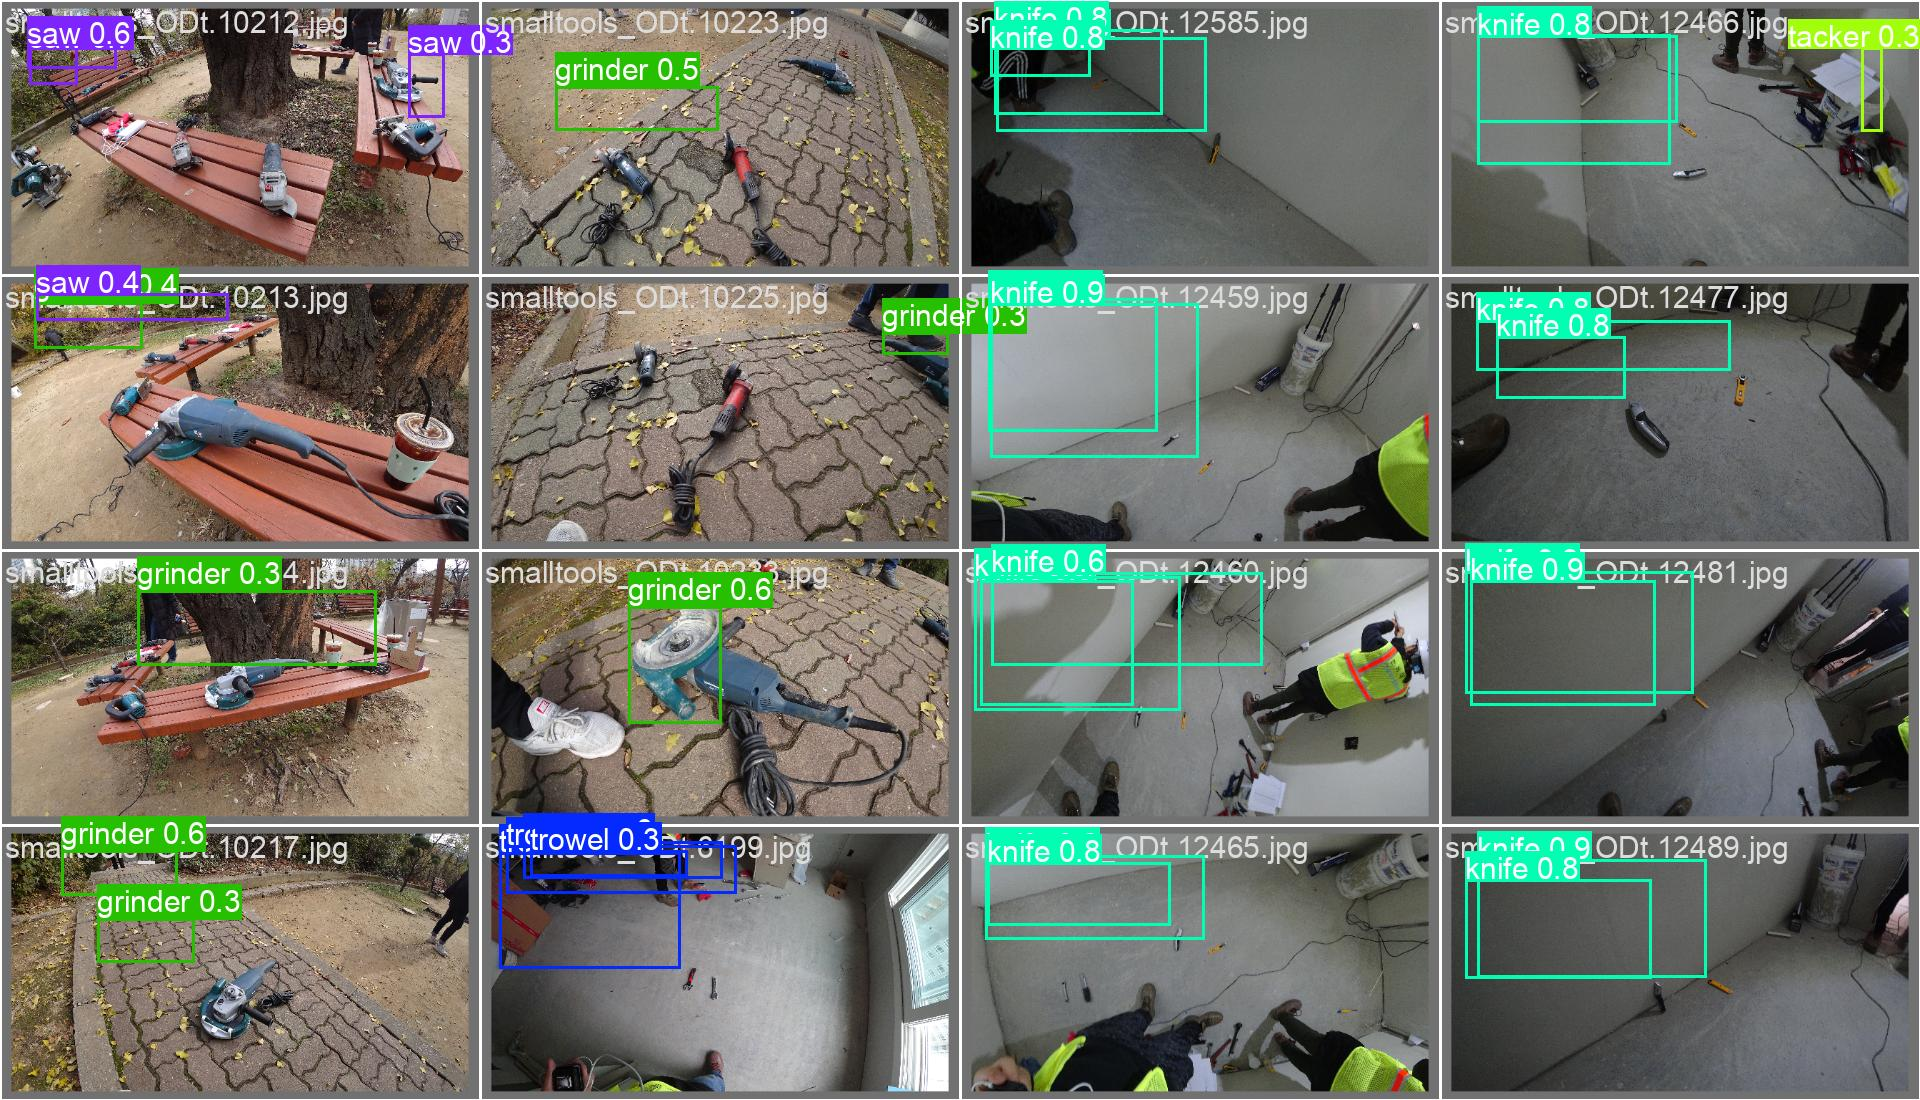
\includegraphics[width=2\textwidth, height=0.55\textheight, keepaspectratio]{val_pred_sgie_equipment.jpg}}
    \end{column}
    \begin{column}{0.48\textwidth}
      \centering
      {\small\textbf{SGIE-Maquinário (9 classes)}}\\[3pt]
      \adjustbox{clip, trim=0 0 {.5\width} 0}{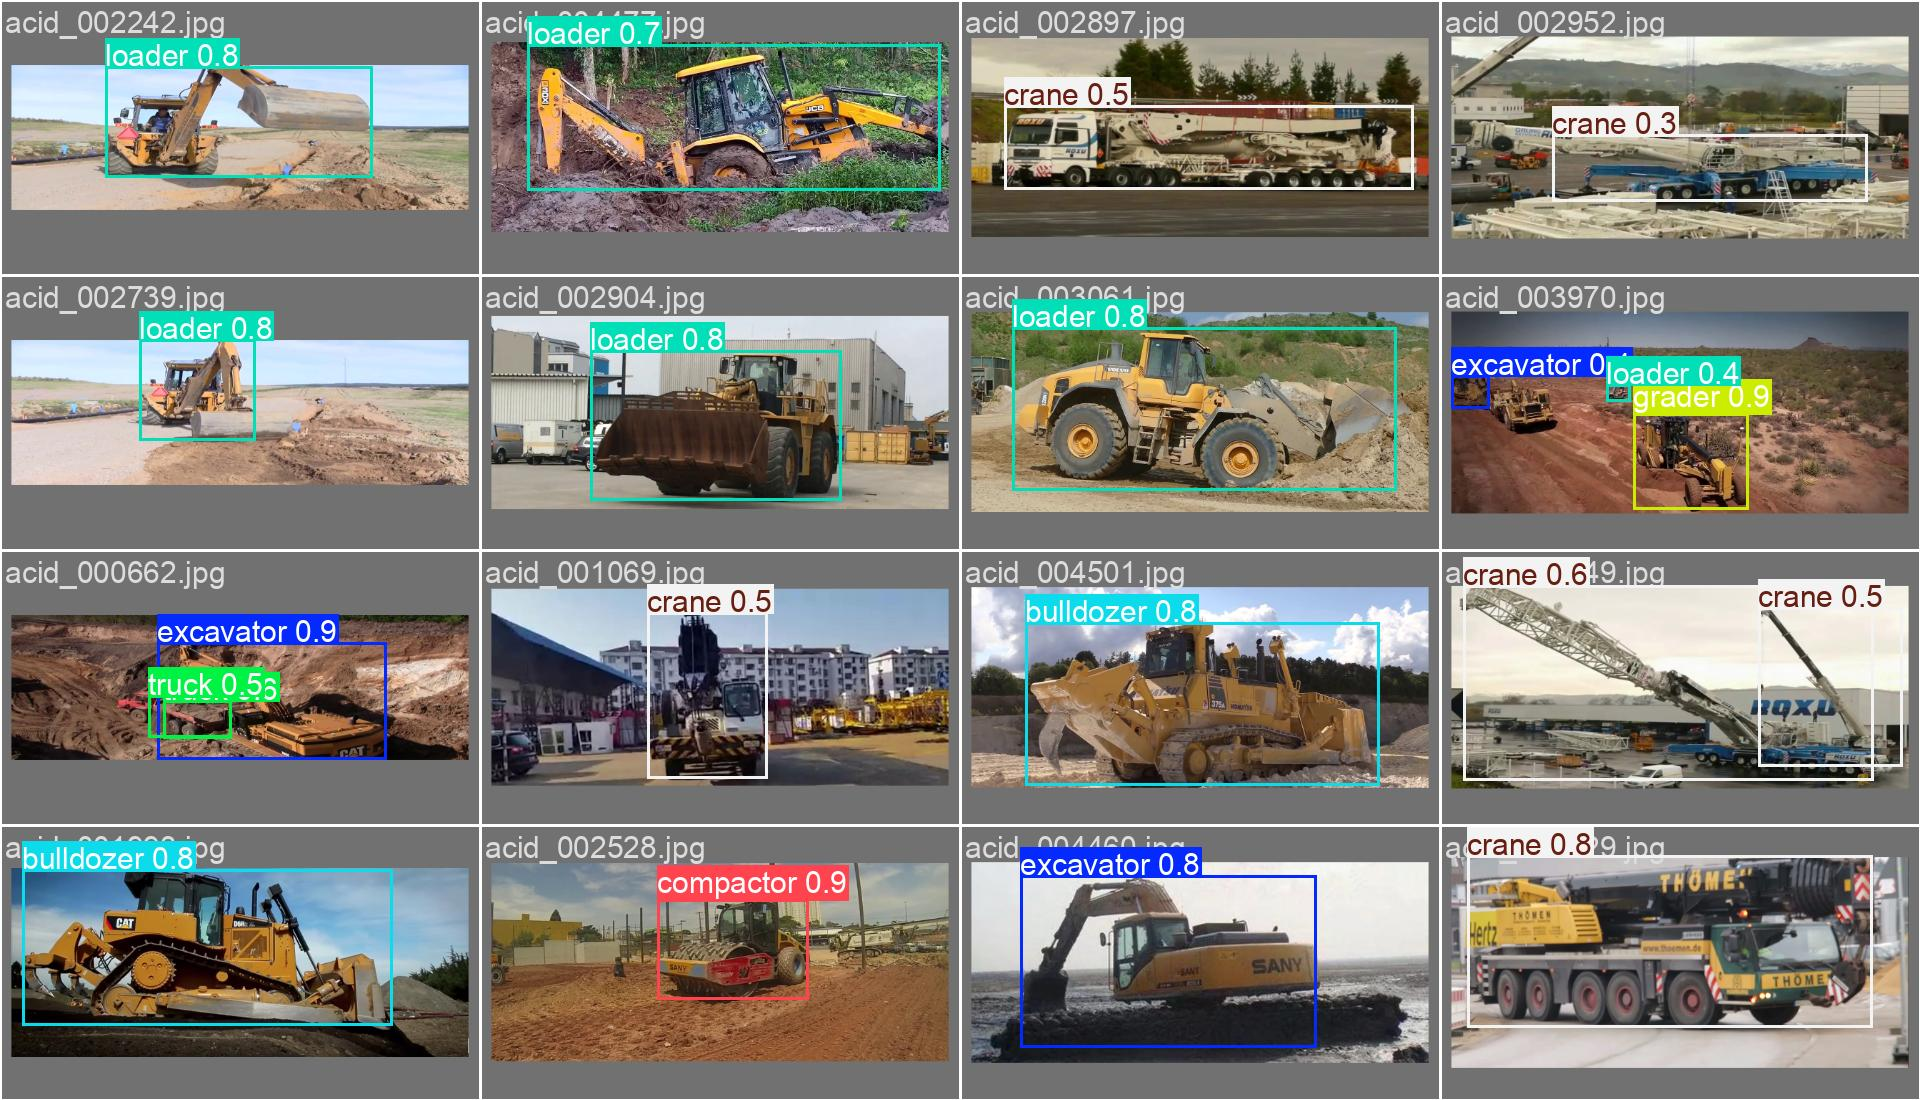
\includegraphics[width=2\textwidth, height=0.55\textheight, keepaspectratio]{val_pred_sgie_machinery.jpg}}
    \end{column}
  \end{columns}

  \vspace{2mm}

  \begin{beamercolorbox}[wd=\textwidth, rounded=true, shadow=false]{block body}
    \centering
    {\footnotesize\color{stagecolor}%
      Predições na validação demonstram detecção de \textbf{múltiplos objetos simultâneos} com classes corretas.
      Modelos diferenciam objetos visualmente similares (Drill vs.\ Grinder).}
  \end{beamercolorbox}
\end{frame}

% ============================================================================
% CAPÍTULO 7 - CONCLUSÃO
% ============================================================================

\section{Conclusão}

% --- Slide 35: Conclusões - Métricas de Impacto ---
\begin{frame}{Conclusões}
  \vfill

  % Row 1: Classes
  \begin{columns}[c]
    \begin{column}{0.18\textwidth}
      \raggedleft
      {\fontsize{26}{28}\selectfont\textcolor{headcolor}{\textbf{46}}}
    \end{column}
    \begin{column}{0.02\textwidth}
      \centering
      \textcolor{arrowcolor}{\rule{0.4pt}{1.5em}}
    \end{column}
    \begin{column}{0.75\textwidth}
      {\small\textbf{Categorias Únicas} --- Cascata PGIE + 3 SGIEs para\\
      \textbf{EPIs}, \textbf{maquinário pesado} e \textbf{ferramentas}.}
    \end{column}
  \end{columns}

  \vspace{3mm}

  % Row 2: mAP
  \begin{columns}[c]
    \begin{column}{0.18\textwidth}
      \raggedleft
      {\fontsize{20}{22}\selectfont\textcolor{inputcolor}{\textbf{0,71--0,84}}}
    \end{column}
    \begin{column}{0.02\textwidth}
      \centering
      \textcolor{arrowcolor}{\rule{0.4pt}{1.5em}}
    \end{column}
    \begin{column}{0.75\textwidth}
      {\small\textbf{mAP@0,5} --- PGIE: 0,83 / EPI: 0,77 / Maq: \textbf{0,84} / Fer: 0,71.}
    \end{column}
  \end{columns}

  \vspace{3mm}

  % Row 3: FPS
  \begin{columns}[c]
    \begin{column}{0.18\textwidth}
      \raggedleft
      {\fontsize{20}{22}\selectfont\textcolor{neckcolor}{\textbf{20\,\scriptsize{FPS}}}}\\[-2pt]
      {\scriptsize\textcolor{neckcolor}{58\,ms}}
    \end{column}
    \begin{column}{0.02\textwidth}
      \centering
      \textcolor{arrowcolor}{\rule{0.4pt}{1.5em}}
    \end{column}
    \begin{column}{0.75\textwidth}
      {\small\textbf{Tempo Real} --- Pipeline completo com 4 modelos simultâneos.}
    \end{column}
  \end{columns}

  \vspace{3mm}

  % Row 4: Power
  \begin{columns}[c]
    \begin{column}{0.18\textwidth}
      \raggedleft
      {\fontsize{26}{28}\selectfont\textcolor{outputcolor}{\textbf{24\,\scriptsize{W}}}}
    \end{column}
    \begin{column}{0.02\textwidth}
      \centering
      \textcolor{arrowcolor}{\rule{0.4pt}{1.5em}}
    \end{column}
    \begin{column}{0.75\textwidth}
      {\small\textbf{Computação na Borda} --- Jetson AGX Xavier, sem nuvem.\\
      Aplicável em canteiros remotos com conectividade limitada.}
    \end{column}
  \end{columns}

  \vfill
\end{frame}

% --- Slide: Objetivos Atingidos (NOVO) ---
\begin{frame}{Objetivos Atingidos}
  \vspace{-2mm}
  {\small\color{sublabelcolor}%
    Mapeamento entre objetivos espec\'{i}ficos (OE1--OE4) e resultados alcan\c{c}ados}

  \vfill
  \begin{center}
    \resizebox{0.95\textwidth}{!}{% ============================================================================
% Diagrama Objetivos Atingidos - OE1 a OE4 com resultados
% Para dissertação de mestrado PPGC/UFRGS
% Uso: % ============================================================================
% Diagrama Objetivos Atingidos - OE1 a OE4 com resultados
% Para dissertação de mestrado PPGC/UFRGS
% Uso: \input{Figures/diagrama_objetivos_atingidos.tex}
% ============================================================================

\begin{tikzpicture}[scale=0.85, transform shape]
  \def\rowH{1.6}
  \def\objW{5.2}
  \def\resW{5.8}
  \def\gap{1.4}

  % --- OE1 ---
  \fill[backbonecolor] (0, 0) rectangle (0.12, -\rowH+0.2);
  \node[fill=backbonecolor!10, rounded corners=3pt, minimum height=12mm, minimum width=\objW cm,
        font=\footnotesize, align=left, anchor=west, draw=backbonecolor!30] (oe1l)
    at (0.25, -\rowH/2+0.1) {
      \textbf{OE1:} Treinar 4 modelos YOLOv8\\
      {\scriptsize PGIE (5 cls) + 3 SGIEs especializados}
    };
  \node[fill=headcolor!10, rounded corners=3pt, minimum height=12mm, minimum width=\resW cm,
        font=\footnotesize, align=left, anchor=west, draw=headcolor!30] (oe1r)
    at (\objW+\gap, -\rowH/2+0.1) {
      {\color{headcolor}$\boldsymbol{\checkmark}$} mAP: 0,83 / 0,77 / 0,84 / 0,71\\
      {\scriptsize 46 categorias \'{u}nicas treinadas e validadas}
    };
  \draw[arrow, line width=0.9pt] (oe1l.east) -- (oe1r.west);

  % --- OE2 ---
  \def\r{1}
  \fill[neckcolor] (0, -\r*\rowH) rectangle (0.12, -\r*\rowH-\rowH+0.2);
  \node[fill=neckcolor!10, rounded corners=3pt, minimum height=12mm, minimum width=\objW cm,
        font=\footnotesize, align=left, anchor=west, draw=neckcolor!30] (oe2l)
    at (0.25, -\r*\rowH-\rowH/2+0.1) {
      \textbf{OE2:} Pipeline DeepStream em cascata\\
      {\scriptsize PGIE $\to$ SGIEs com rastreamento}
    };
  \node[fill=headcolor!10, rounded corners=3pt, minimum height=12mm, minimum width=\resW cm,
        font=\footnotesize, align=left, anchor=west, draw=headcolor!30] (oe2r)
    at (\objW+\gap, -\r*\rowH-\rowH/2+0.1) {
      {\color{headcolor}$\boldsymbol{\checkmark}$} 20 FPS / 58\,ms lat\^{e}ncia end-to-end\\
      {\scriptsize Pipeline funcional com 4 modelos simult\^{a}neos}
    };
  \draw[arrow, line width=0.9pt] (oe2l.east) -- (oe2r.west);

  % --- OE3 ---
  \def\r{2}
  \fill[detectioncolor] (0, -\r*\rowH) rectangle (0.12, -\r*\rowH-\rowH+0.2);
  \node[fill=detectioncolor!10, rounded corners=3pt, minimum height=12mm, minimum width=\objW cm,
        font=\footnotesize, align=left, anchor=west, draw=detectioncolor!30] (oe3l)
    at (0.25, -\r*\rowH-\rowH/2+0.1) {
      \textbf{OE3:} Parser C++ YOLOv8--DeepStream\\
      {\scriptsize Roteamento PGIE $\to$ SGIEs por classe}
    };
  \node[fill=headcolor!10, rounded corners=3pt, minimum height=12mm, minimum width=\resW cm,
        font=\footnotesize, align=left, anchor=west, draw=headcolor!30] (oe3r)
    at (\objW+\gap, -\r*\rowH-\rowH/2+0.1) {
      {\color{headcolor}$\boldsymbol{\checkmark}$} Biblioteca .so compilada e integrada\\
      {\scriptsize Decodifica\c{c}\~{a}o anchor-free + NMS + roteamento}
    };
  \draw[arrow, line width=0.9pt] (oe3l.east) -- (oe3r.west);

  % --- OE4 ---
  \def\r{3}
  \fill[outputcolor] (0, -\r*\rowH) rectangle (0.12, -\r*\rowH-\rowH+0.2);
  \node[fill=outputcolor!10, rounded corners=3pt, minimum height=12mm, minimum width=\objW cm,
        font=\footnotesize, align=left, anchor=west, draw=outputcolor!30] (oe4l)
    at (0.25, -\r*\rowH-\rowH/2+0.1) {
      \textbf{OE4:} Avalia\c{c}\~{a}o de desempenho\\
      {\scriptsize Acur\'{a}cia, velocidade e recursos}
    };
  \node[fill=headcolor!10, rounded corners=3pt, minimum height=12mm, minimum width=\resW cm,
        font=\footnotesize, align=left, anchor=west, draw=headcolor!30] (oe4r)
    at (\objW+\gap, -\r*\rowH-\rowH/2+0.1) {
      {\color{headcolor}$\boldsymbol{\checkmark}$} GPU 82\% | RAM 18\% | 24\,W\\
      {\scriptsize M\'{e}tricas completas no Jetson AGX Xavier}
    };
  \draw[arrow, line width=0.9pt] (oe4l.east) -- (oe4r.west);
\end{tikzpicture}

% ============================================================================

\begin{tikzpicture}[scale=0.85, transform shape]
  \def\rowH{1.6}
  \def\objW{5.2}
  \def\resW{5.8}
  \def\gap{1.4}

  % --- OE1 ---
  \fill[backbonecolor] (0, 0) rectangle (0.12, -\rowH+0.2);
  \node[fill=backbonecolor!10, rounded corners=3pt, minimum height=12mm, minimum width=\objW cm,
        font=\footnotesize, align=left, anchor=west, draw=backbonecolor!30] (oe1l)
    at (0.25, -\rowH/2+0.1) {
      \textbf{OE1:} Treinar 4 modelos YOLOv8\\
      {\scriptsize PGIE (5 cls) + 3 SGIEs especializados}
    };
  \node[fill=headcolor!10, rounded corners=3pt, minimum height=12mm, minimum width=\resW cm,
        font=\footnotesize, align=left, anchor=west, draw=headcolor!30] (oe1r)
    at (\objW+\gap, -\rowH/2+0.1) {
      {\color{headcolor}$\boldsymbol{\checkmark}$} mAP: 0,83 / 0,77 / 0,84 / 0,71\\
      {\scriptsize 46 categorias \'{u}nicas treinadas e validadas}
    };
  \draw[arrow, line width=0.9pt] (oe1l.east) -- (oe1r.west);

  % --- OE2 ---
  \def\r{1}
  \fill[neckcolor] (0, -\r*\rowH) rectangle (0.12, -\r*\rowH-\rowH+0.2);
  \node[fill=neckcolor!10, rounded corners=3pt, minimum height=12mm, minimum width=\objW cm,
        font=\footnotesize, align=left, anchor=west, draw=neckcolor!30] (oe2l)
    at (0.25, -\r*\rowH-\rowH/2+0.1) {
      \textbf{OE2:} Pipeline DeepStream em cascata\\
      {\scriptsize PGIE $\to$ SGIEs com rastreamento}
    };
  \node[fill=headcolor!10, rounded corners=3pt, minimum height=12mm, minimum width=\resW cm,
        font=\footnotesize, align=left, anchor=west, draw=headcolor!30] (oe2r)
    at (\objW+\gap, -\r*\rowH-\rowH/2+0.1) {
      {\color{headcolor}$\boldsymbol{\checkmark}$} 20 FPS / 58\,ms lat\^{e}ncia end-to-end\\
      {\scriptsize Pipeline funcional com 4 modelos simult\^{a}neos}
    };
  \draw[arrow, line width=0.9pt] (oe2l.east) -- (oe2r.west);

  % --- OE3 ---
  \def\r{2}
  \fill[detectioncolor] (0, -\r*\rowH) rectangle (0.12, -\r*\rowH-\rowH+0.2);
  \node[fill=detectioncolor!10, rounded corners=3pt, minimum height=12mm, minimum width=\objW cm,
        font=\footnotesize, align=left, anchor=west, draw=detectioncolor!30] (oe3l)
    at (0.25, -\r*\rowH-\rowH/2+0.1) {
      \textbf{OE3:} Parser C++ YOLOv8--DeepStream\\
      {\scriptsize Roteamento PGIE $\to$ SGIEs por classe}
    };
  \node[fill=headcolor!10, rounded corners=3pt, minimum height=12mm, minimum width=\resW cm,
        font=\footnotesize, align=left, anchor=west, draw=headcolor!30] (oe3r)
    at (\objW+\gap, -\r*\rowH-\rowH/2+0.1) {
      {\color{headcolor}$\boldsymbol{\checkmark}$} Biblioteca .so compilada e integrada\\
      {\scriptsize Decodifica\c{c}\~{a}o anchor-free + NMS + roteamento}
    };
  \draw[arrow, line width=0.9pt] (oe3l.east) -- (oe3r.west);

  % --- OE4 ---
  \def\r{3}
  \fill[outputcolor] (0, -\r*\rowH) rectangle (0.12, -\r*\rowH-\rowH+0.2);
  \node[fill=outputcolor!10, rounded corners=3pt, minimum height=12mm, minimum width=\objW cm,
        font=\footnotesize, align=left, anchor=west, draw=outputcolor!30] (oe4l)
    at (0.25, -\r*\rowH-\rowH/2+0.1) {
      \textbf{OE4:} Avalia\c{c}\~{a}o de desempenho\\
      {\scriptsize Acur\'{a}cia, velocidade e recursos}
    };
  \node[fill=headcolor!10, rounded corners=3pt, minimum height=12mm, minimum width=\resW cm,
        font=\footnotesize, align=left, anchor=west, draw=headcolor!30] (oe4r)
    at (\objW+\gap, -\r*\rowH-\rowH/2+0.1) {
      {\color{headcolor}$\boldsymbol{\checkmark}$} GPU 82\% | RAM 18\% | 24\,W\\
      {\scriptsize M\'{e}tricas completas no Jetson AGX Xavier}
    };
  \draw[arrow, line width=0.9pt] (oe4l.east) -- (oe4r.west);
\end{tikzpicture}
}
  \end{center}
  \vfill

  \begin{beamercolorbox}[wd=\textwidth, rounded=true, shadow=false]{block body}
    \centering
    {\footnotesize\color{stagecolor}%
      Todos os \textbf{4 objetivos espec\'{i}ficos} foram atingidos --- sistema funcional validado no Jetson AGX Xavier}
  \end{beamercolorbox}
\end{frame}

% --- Slide 36: Limitações e Trabalhos Futuros ---
\begin{frame}{Limitações e Trabalhos Futuros}
  \vspace{-2mm}
  \begin{columns}[t]
    \begin{column}{0.46\textwidth}
      {\small\textcolor{skipcolor}{\textbf{Limitações}}}
      \vspace{1mm}
      \begin{itemize}\setlength{\itemsep}{0.5mm}\scriptsize
        \item \textbf{Propagação de erros} --- cobertura efetiva 0,59--0,76
        \item \textbf{Objetos pequenos} --- AP $<$ 0,60 (Cutter, Trowel)
        \item \textbf{Validação controlada} --- benchmark, sem canteiro real
        \item \textbf{Dataset sem dados locais} --- canteiros BR não representados
        \item \textbf{Desbalanceamento} --- NO-Safety Vest: AP=0,236
      \end{itemize}
    \end{column}
    \begin{column}{0.50\textwidth}
      {\small\textcolor{headcolor}{\textbf{Trabalhos Futuros}}}
      \vspace{1mm}
      \begin{itemize}\setlength{\itemsep}{0.5mm}\scriptsize
        \item \textcolor{headcolor}{$\checkmark$} \textbf{SAHI} para objetos pequenos
        \item \textcolor{headcolor}{$\checkmark$} \textbf{Dataset brasileiro} com classes sub-representadas
        \item \textcolor{headcolor}{$\checkmark$} \textbf{YOLOv9 / YOLOv10 / RT-DETR}
        \item \textcolor{headcolor}{$\checkmark$} \textbf{Piloto em canteiro real} (NR-18)
        \item \textcolor{headcolor}{$\checkmark$} \textbf{Quantização INT8 + DLA} ($>$30 FPS)
      \end{itemize}
    \end{column}
  \end{columns}
  \vfill
\end{frame}

% --- Slide 37: Impacto e Aplicabilidade ---
\begin{frame}{Impacto e Aplicabilidade Real}
  \vspace{-1mm}

  \begin{columns}[c]
    \begin{column}{0.48\textwidth}
      \centering
      \colorbox{skipcolor!10}{%
        \parbox{0.88\textwidth}{\centering\vspace{2pt}
          {\fontsize{22}{24}\selectfont\textcolor{skipcolor}{\textbf{2.538}}}\\[1pt]
          {\footnotesize mortes na construção civil\\brasileira (2012--2021)}\\[1pt]
          {\tiny Fonte: SmartLab / MPT / OIT}
        \vspace{2pt}}%
      }

      \vspace{2mm}

      \colorbox{gridcolor!15}{%
        \parbox{0.88\textwidth}{\centering\vspace{2pt}
          {\small\textbf{NR-18}}\\[1pt]
          {\footnotesize Conformidade automatizada\\com norma de segurança}
        \vspace{2pt}}%
      }
    \end{column}
    \begin{column}{0.48\textwidth}
      \centering
      {\small\textbf{Cenários de Implantação}}

      \vspace{2mm}

      \begin{itemize}\setlength{\itemsep}{1.5mm}\footnotesize
        \item \textbf{Grandes construtoras} --- {\scriptsize alertas 24h}
        \item \textbf{Obras públicas} --- {\scriptsize fiscalização NR-18}
        \item \textbf{Canteiros remotos} --- {\scriptsize Edge AI a 24W}
        \item \textbf{Seguradoras} --- {\scriptsize avaliação de risco}
      \end{itemize}
    \end{column}
  \end{columns}

  \vspace{2mm}

  \begin{beamercolorbox}[wd=\textwidth, rounded=true, shadow=false]{block body}
    \centering
    {\footnotesize\color{stagecolor}%
      \textbf{Tecnologia acessível}: Jetson AGX Xavier ({\raise.17ex\hbox{$\scriptstyle\sim$}}US\$\,700) + câmera IP --- custo operacional mínimo.}
  \end{beamercolorbox}
  \vfill
\end{frame}

% --- Slide 38: Encerramento ---
{
\setbeamertemplate{footline}{}
\begin{frame}[plain]
  \vfill
  \begin{center}
    {\fontsize{40}{44}\selectfont\color{stagecolor}\textbf{Obrigado!}}

    \vspace{8mm}

    {\Large\color{arrowcolor} Perguntas?}

    \vspace{10mm}

    {\small\color{stagecolor}\textbf{Monitoramento de Segurança em Canteiros de Obra utilizando\\
    Inferência Multiestágio em Inteligência Artificial na Borda}}

    \vspace{8mm}

    {\normalsize Luiz Guilherme Martinho Sampaio Ito}\\[3pt]
    {\small\color{arrowcolor} Orientador: Prof.~Dr.~José Rodrigo Furlanetto de Azambuja}\\[6pt]
    {\footnotesize\color{inputcolor} guilherme.ito@ufrgs.br}\\[8pt]
    {\footnotesize Instituto de Informática --- UFRGS\\
    Programa de Pós-Graduação em Computação\\[2pt]
    Março de 2026}
  \end{center}
  \vfill
\end{frame}
}


\end{document}
